 % The main file for CAMP reports
 % Don't put any content in here. 
 % Don't even include content files by using \input or \inlcude. 
 % Put your content to TEXT.TEX or include it there using \input.
 % Uses:
 %		SETTINGS.TEX	contains the settings for this document
 %		COMMANDS.TEX	contains commands which can be used while writing
 %		INFO.TEX			contains the author, title and so on for the cover
 %		COVER.TEX			formats\documentclass[10pt]{?} the front cover of the document
 %		ABSTRACT.TEX	contains the abstract to be included (if needed)
 %		TEXT.TEX			contains the actual content of the document
 %		BIB.BIB				containt the BibTeX entries for the document
 
 
%% Draft document mode
%% Final document
\documentclass[11pt,a4paper,bibtotoc,idxtotoc,headsepline,footsepline,footexclude,BCOR12mm,DIV13]{scrbook}

\usepackage{multirow}
\usepackage{listings}
\usepackage{color}

\definecolor{mygreen}{rgb}{0,0.6,0}
\definecolor{mygray}{rgb}{0.5,0.5,0.5}
\definecolor{mymauve}{rgb}{0.58,0,0.82}
\lstset{ %
  backgroundcolor=\color{white},   % choose the background color
  basicstyle=\footnotesize,        % size of fonts used for the code
  breaklines=true,                 % automatic line breaking only at whitespace
  captionpos=b,                    % sets the caption-position to bottom
  commentstyle=\color{mygreen},    % comment style
  escapeinside={\%*}{*)},          % if you want to add LaTeX within your code
  keywordstyle=\color{blue},       % keyword style
  stringstyle=\color{mymauve},     % string literal style
}

%\documentclass[11pt,a4paper,bibtotoc,idxtotoc,headsepline,footsepline,footexclude,BCOR20mm,DIV10]{scrbook}

% KOMA-Optionen:
%  bibtotoc: include bibliography in table of contents
%  idxtotoc: include index in table of contents
%  headsepline: use horizontalline under heading
%  BCOR: binding correcion (Bindungskorrektur) (e.g.: BCOR5mm)
%  DIV: Number of sheet sections (used for layout) (e.g.: DIV12) 


% include title and author information for the cover
% Set here the title, authors and other stuff to be used for the cover
% This file is used by MAIN.TEX

% set title, authors and stuff for the cover
\def\doctype{Master's Thesis in Informatics}
\def\title{Materialized views with Apache Spark}
\def\titleGer{Materialisierte views mit Apache Spark}
\def\author{Saroj Gautam}
\def\date{August 15th, 2016}

% text to appear in the footer
\def\footertext{}

% include settings
% Included by MAIN.TEX
% Defines the settings for the CAMP report document

\renewcommand{\sectfont}{\normalfont \bfseries}        % Schriftart der Kopfzeile

% manipulate footer
\usepackage{scrpage2}
\pagestyle{scrheadings}
\ifoot[\footertext]{\footertext} % \footertext set in INFO.TEX
%\setkomafont{pagehead}{\normalfont\rmfamily}
\setkomafont{pagenumber}{\normalfont\rmfamily}

%% allow sophisticated control structures
\usepackage{ifthen}

% use Palatino as default font
\usepackage{palatino}

% enable special PostScript fonts
\usepackage{pifont}

% make thumbnails
\usepackage{thumbpdf}

%to use the subfigures
%\usepackage{subfigure}
\usepackage{caption}
\usepackage{subcaption}


\usepackage{colortbl}


%% show program code\ldots
%\usepackage{verbatim}
%\usepackage{program}

\usepackage{listings}


%% enable TUM symbols on title page
\usepackage{styles/tumlogo}


\usepackage{multirow}

%% use colors
\usepackage{color}

%% make fancy math
\usepackage{amsmath}
\usepackage{amsfonts}
\usepackage{amssymb}
\usepackage{textcomp}
\usepackage{yhmath} % f�r die adots 
%% mark text as preliminary
%\usepackage[draft,german,scrtime]{prelim2e}

%% create an index
\usepackage{makeidx}

% for the program environment
\usepackage{float}

%% load german babel package for german abstract
%\usepackage[german,american]{babel}
\usepackage[german,english]{babel}
\selectlanguage{english}

% use german characters as well
\usepackage[latin1]{inputenc}       % allow Latin1 characters

% use initals dropped caps - doesn't work with PDF
%\usepackage{dropping}

% Load the package
\usepackage{glossaries}

\usepackage{styles/shortoverview}
%----------------------------------------------------
%      Graphics and Hyperlinks
%----------------------------------------------------

%% check for pdfTeX
\ifx\pdftexversion\undefined
 %% use PostScript graphics
 \usepackage[dvips]{graphicx}
 \DeclareGraphicsExtensions{.eps,.epsi}
 \graphicspath{{figures/}{figures/review}} 
 %% allow rotations
 \usepackage{rotating}
 %% mark pages as draft copies
 %\usepackage[english,all,light]{draftcopy}
 %% use hypertex version of hyperref
 \usepackage[hypertex,hyperindex=false,colorlinks=false]{hyperref}
\else %% reduce output size \pdfcompresslevel=9
 %% declare pdfinfo
 %\pdfinfo { 
 %  /Title (my title) 
 %  /Creator (pdfLaTeX) 
 %  /Author (my name) 
 %  /Subject (my subject	) 
 %  /Keywords (my keywords)
 %}
 %% use pdf or jpg graphics
 \usepackage[pdftex]{graphicx}
 \DeclareGraphicsExtensions{.jpg,.JPG,.png,.pdf,.eps}
 \graphicspath{{figures/}} 
 
 %% Load float package, for enabling floating extensions
 \usepackage{float}
 
 %% allow rotations
 \usepackage{rotating}
 %% use pdftex version of hyperref
 \usepackage[pdftex,colorlinks=true,linkcolor=black,citecolor=black,%
 anchorcolor=black,urlcolor=black,bookmarks=true,%
 bookmarksopen=true,bookmarksopenlevel=0,plainpages=false%
 bookmarksnumbered=true,hyperindex=false,pdfstartview=%
 ]{hyperref}
%
%\usepackage[pdftex,colorlinks=false,linkcolor=red,citecolor=red,%
% anchorcolor=red,urlcolor=red,bookmarks=true,%
% bookmarksopen=true,bookmarksopenlevel=0,plainpages=false%
% bookmarksnumbered=true,hyperindex=false,pdfstartview=%
% ]{hyperref}
\fi




%% Fancy chapters
%\usepackage[Lenny]{fncychap}
%\usepackage[Glenn]{fncychap}
%\usepackage[Bjarne]{fncychap}

%\usepackage[avantgarde]{quotchap}

% set the bibliography style
%\bibliographystyle{styles/bauermaNum}
%\bibliographystyle{alpha}
\bibliographystyle{plain}

% include commands
% Commands to be used within the TUM report document
% Included by MAIN.TEX
% Please include your own cool commands here. 
% Be only sure to comment it sufficiently so others can use it.

%-------------------------------------------------------------
%                      Own Commands
%-------------------------------------------------------------


%-------------------------------------------------------------
% math stuff -------------------------------------------------

% nice R, N, C
\newcommand{\nat}{\mathbb{N}}
\newcommand{\real}{\mathbb{R}}
\newcommand{\compl}{\mathbb{C}}



% norm
\newcommand{\norm}[1]{\left\| #1 \right\|}

% un demi
\newcommand{\half}{\frac{1}{2}}

% parantheses
\newcommand{\parenth}[1]{ \left( #1 \right) }
\newcommand{\bracket}[1]{ \left[ #1 \right] }
\newcommand{\accolade}[1]{ \left\{ #1 \right\} }
%\newcommand{\angle}[1]{ \left\langle  #1 \right\rangle }

% partial derivative: %#1 function, #2 which variable
% simple / single line version
\newcommand{\pardevS}[2]{ \delta_{#1} f(#2) }
% fraction version
\newcommand{\pardevF}[2]{ \frac{\partial #1}{\partial #2} }

% render vectors: 3 and 4 dimensional
\newcommand{\veciii}[3]{\left[ \begin{array}[h]{c} #1 \\ #2 \\ #3	\end{array} \right]}
\newcommand{\veciv}[4]{\left[ \begin{array}[h]{c} #1 \\ #2 \\ #3 \\ #4	\end{array} \right]}

% render matrices: 3  dimensional (arguments in row first order)
\newcommand{\matiii}[9]{\left[ \begin{array}[h]{ccc} #1 & #2 & #3 \\ #4 & #5 & #6 \\ #7 & #8 & #9	\end{array} \right]}
%DOESN'T WORK,DON'T KNOW WHY \newcommand{\mativ}[16]{\left[ \begin{array}[h]{cccc} #1 & #2 & #3 & #4 \\ #5 & #6 & #7 & #8 \\ #9 & #10 & #11 & #12 \\ #13 & #14 & #15 & #16 \end{array} \right]}


%-------------------------------------------------------------
%-------------------------------------------------------------


%-------------------------------------------------------------
% some abreviations ------------------------------------------
\newcommand{\Reg}{$^{\textregistered}$}
\newcommand{\reg}{$^{\textregistered}$ }
\newcommand{\Tm}{\texttrademark}
\newcommand{\tm}{\texttrademark~}
\newcommand {\bsl} {$\backslash$}

%-------------------------------------------------------------
%-------------------------------------------------------------


%-------------------------------------------------------------
% formating --------------------------------------------------

% Theorem & Co environments and counters
\newtheorem{theorem}{Theorem}[chapter]
\newtheorem{lemma}[theorem]{Lemma}
\newtheorem{corollary}[theorem]{Corollary}
\newtheorem{remark}[theorem]{Remark}
\newtheorem{definition}[theorem]{Definition}
\newtheorem{equat}[theorem]{Equation}
\newtheorem{example}[theorem]{Example}
\newtheorem{algorithm}[theorem]{Algorithm}

% inserting figures
\newcommand{\insertfigure}[4]{ % Filename, Caption, Label, Width percent of textwidth
	\begin{figure}[htbp]
		\begin{center}
			\includegraphics[width=#4\textwidth]{#1}
		\end{center}
		\vspace{-0.4cm}
		\caption{#2}
		\label{#3}
	\end{figure}
}




% referecing figures

\newcommand{\refFigure}[1]{ %label
	figure \ref{#1}
}
\newcommand{\refChapter}[1]{ %label
	chapter \ref{#1}
}

\newcommand{\refSection}[1]{ %label
	section \ref{#1}
}

\newcommand{\refParagraph}[1]{ %label
	paragraph \ref{#1}
}

\newcommand{\refEquation}[1]{ %label
	equation \ref{#1}
}

\newcommand{\refTable}[1]{ %label
	table \ref{#1}
}




\newcommand{\rigidTransform}[2]
{
	${}^{#2}\!\mathbf{H}_{#1}$
}

%code, in typewriter
\newcommand{\code}[1]
 {\texttt{#1}}

% comment that appears on the border - very practical !!!
\newcommand{\comment}[1]{\marginpar{\raggedright \noindent \footnotesize {\sl #1} }}

% page clearing
\newcommand{\clearemptydoublepage}{%
  \ifthenelse{\boolean{@twoside}}{\newpage{\pagestyle{empty}\cleardoublepage}}%
  {\clearpage}}


%-------------------------------------------------------------
%-------------------------------------------------------------


\newcommand{\etAl}{\emph{et al.}\mbox{ }}


%\makeindex
	%% inter line spacing
%\linespread{1.0}

\makeglossary

\begin{document}

	\frontmatter
	
	
	% The front cover for the TUM report document.
% Included by MAIN.TEX


%--------------------------------------------------
% The Front Cover
%--------------------------------------------------

% The front cover for the TUM document.
% Included by MAIN.TEX


%--------------------------------------------------
% The Front Cover
%--------------------------------------------------

% correct BCOR - undo at the end !!!
\def\bcorcor{0.15cm}
\addtolength{\hoffset}{\bcorcor}

\thispagestyle{empty}

 \vspace{4cm}
\begin{center}
	       \oTUM{4cm}
	   
	   \vspace{5mm}     
	   \huge FAKULT{\"A}T F{\"U}R INFORMATIK\\ 
	   \vspace{0.5cm}
	 \large DER TECHNISCHEN UNIVERSIT{\"A}T M{\"U}NCHEN\\
    \vspace{1mm}
        
	\end{center}
		

\vspace{15mm}
\begin{center}

   {\Large \doctype}

  \vspace{20mm}
  
  {\huge\bf \title}\\%[3ex]
  
  
  \vspace{15mm}
  
  
  {\LARGE  \author}
  
  \vspace{10mm}
  
  \begin{figure}[h!]
  \centering
   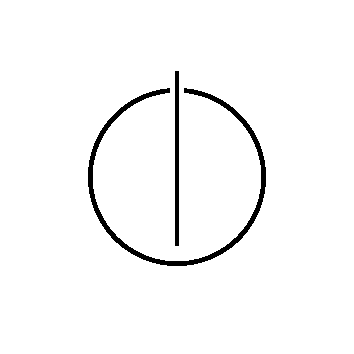
\includegraphics[width=4cm]{styles/informat.png}
  \end{figure}
  
  \end{center}
%	\clearemptydoublepage
	
	%% The titlepage for the CAMP report document.
% Included by MAIN.TEX


%--------------------------------------------------
% The title page
%--------------------------------------------------

% correct BCOR - undo at the end !!!
\def\bcorcor{0.15cm}
\addtolength{\hoffset}{\bcorcor}

\thispagestyle{empty}

 \vspace{10mm}
\begin{center}
	       \oTUM{4cm}
	   
	   \vspace{5mm}     
	   \huge FAKULT{\"A}T F{\"U}R INFORMATIK\\ 
	   \vspace{0.5cm}
	 \large DER TECHNISCHEN UNIVERSIT{\"A}T M{\"U}NCHEN\\
        
	\end{center}
		

\vspace{10mm}
\begin{center}

   {\Large \doctype}

  \vspace{10mm}
  
  {\LARGE \title}\\
  
  
  \vspace{10mm}
  
  
  {\LARGE  \titleGer}\\
  
  
  \vspace{10mm}

    %\hfill
    \begin{tabular}{ll}
	   \Large Author:     & \Large \author \\[2mm]
	   \Large Supervisor:    & \Large Prof. Dr. Hans-Arno Jacobsen \\[2mm]				
	   \Large Advisor:	& \Large M. Sc. Jan Adler\\[2mm]
	   \Large Date:       & \Large August 15, 2016
	 \end{tabular}
	 
	 \vspace{5mm}
	 
	 \begin{figure}[h!]
  \centering
   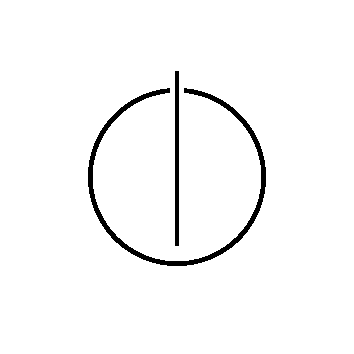
\includegraphics[width=4cm]{styles/informat.png}
  \end{figure}
   

\end{center}

% undo BCOR correction
\addtolength{\hoffset}{\bcorcor}
	
	
%	\input{components/cover_maschmeyer}
	\clearemptydoublepage
	
	% The titlepage for the CAMP report document.
% Included by MAIN.TEX


%--------------------------------------------------
% The title page
%--------------------------------------------------

% correct BCOR - undo at the end !!!
\def\bcorcor{0.15cm}
\addtolength{\hoffset}{\bcorcor}

\thispagestyle{empty}

 \vspace{10mm}
\begin{center}
	       \oTUM{4cm}
	   
	   \vspace{5mm}     
	   \huge FAKULT{\"A}T F{\"U}R INFORMATIK\\ 
	   \vspace{0.5cm}
	 \large DER TECHNISCHEN UNIVERSIT{\"A}T M{\"U}NCHEN\\
        
	\end{center}
		

\vspace{10mm}
\begin{center}

   {\Large \doctype}

  \vspace{10mm}
  
  {\LARGE \title}\\
  
  
  \vspace{10mm}
  
  
  {\LARGE  \titleGer}\\
  
  
  \vspace{10mm}

    %\hfill
    \begin{tabular}{ll}
	   \Large Author:     & \Large \author \\[2mm]
	   \Large Supervisor:    & \Large Prof. Dr. Hans-Arno Jacobsen \\[2mm]				
	   \Large Advisor:	& \Large M. Sc. Jan Adler\\[2mm]
	   \Large Date:       & \Large August 15, 2016
	 \end{tabular}
	 
	 \vspace{5mm}
	 
	 \begin{figure}[h!]
  \centering
   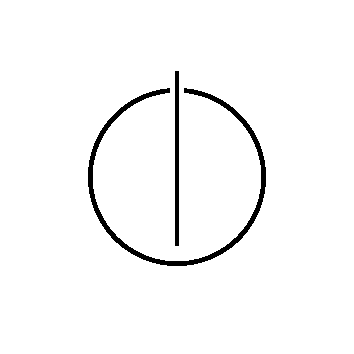
\includegraphics[width=4cm]{styles/informat.png}
  \end{figure}
   

\end{center}

% undo BCOR correction
\addtolength{\hoffset}{\bcorcor}
	
	
	\clearemptydoublepage


\thispagestyle{empty}
\selectlanguage{english}
	\vspace*{0.8\textheight}
	\noindent
	I assure the single handed composition of this master's thesis, only supported by declared resources.
	\newline
	\newline
	\newline
	\noindent
	M{\"u}nchen, August 15th, 2016 \hspace{5cm} \author
\selectlanguage{english}
\newpage
	
	\clearemptydoublepage
\phantomsection
\addcontentsline{toc}{chapter}{Acknowledgements}	


%\chapter*{Acknowledgements}

\vspace*{2cm}

\begin{center}
{\Large \bf Acknowledgments}
\end{center}

\vspace{1cm}

I would first like to thank my advisor Jan Adler for providing me the opportunity to work on an interesting topic and supervising me throughout the research. 
\newline

I thank Prof. Dr. Hans-Arno Jacobsen for providing me an opportunity to write my thesis under the Chair of Distributed Systems. I thank my advisor for providing me valuable feedbacks and suggestion from the start to the end of the thesis.
\newline

I would like to thank my family for giving me the motivation and moral support. I would also like to thank my friends Suvash Sedhain and Niroj Sapkota for their constant support and motivation. And special thanks to my friends for creating a positive environment by cracking jokes and taking off the pressure during coffee breaks.

	
	% Abstract for the TUM report document
% Included by MAIN.TEX


\clearemptydoublepage
\phantomsection
\addcontentsline{toc}{chapter}{Abstract}	





\vspace*{2cm}
\begin{center}
{\Large \bf Abstract}
\end{center}
\vspace{1cm}

% In today's world where billions of people exchange information online, service providers like Facebook, Twitter, Whatsapp store and process tremendous amount of data. Those service providers need distributed scalable storage systems to store and process big volume of data. Even though data are stored in a distributed storage systems, still the huge size of data are bottleneck for performance optimization. Scanning tens of millions rows and few million columns each time are expensive in terms of execution time and processing power. $Materialized$ $Views$ solve this problem by precomputing expensive queries and storing result in a physical table or disk. One of the bottleneck for this approach is constantly maintaining consistency between base table and view table. We propose a $Incremental$ $View$ $Maintenance$ approach to maintain consistency between base table and view table.


In today's world, billions of people exchange information online. Service providers like Facebook, Twitter, Whatsapp store and process tremendous amount of data. Those service providers need distributed scalable storage systems to store and process a big volume of data. Even though data are stored in a distributed storage systems, still the huge size of data can be a bottleneck regarding performance optimization. Scanning tens of millions of rows and few million columns each time are expensive regarding execution time and processing power. $Materialized$ $Views$ solve this problem by pre-computing expensive queries and storing the result in a physical table or disk. One of the bottlenecks for this approach is constantly maintaining consistency between the base table and the view table. In this thesis, we propose a $Incremental$ $View$ $Maintenance$ approach to maintain consistency between the base table and the view table.
	
	% Abstract for the TUM report document
% Included by MAIN.TEX


\clearemptydoublepage
\phantomsection
\addcontentsline{toc}{chapter}{Abbreviation}	





\vspace*{2cm}
\begin{center}
{\Large \bf Abbreviation}
\end{center}
\vspace{1cm}

    % Acronym definitions
	\newacronym{utc}{UTC}{Coordinated Universal Time}
	\newacronym{adt}{ADT}{Atlantic Daylight Time}
	\newacronym{est}{EST}{Eastern Standard Time}
	
	% Use the acronyms
	\gls{utc} is 3 hours behind \gls{adt} and 10 hours ahead of \gls{est}.
	
	%Print the glossary
	\printglossaries
	




	\tableofcontents
  
 % \clearemptydoublepage

\phantomsection
\addcontentsline{toc}{chapter}{Outline of the Thesis}

\begin{center}
	\huge{Outline of the Thesis}
\end{center}




%--------------------------------------------------------------------
\section*{Part I: Introduction and Theory}

\noindent {\scshape Chapter 1: Introduction}  \vspace{1mm}

\noindent  This chapter presents an overview of the thesis and it purpose. Furthermore, it will discuss the sense of life in a very general approach.  \\

\noindent {\scshape Chapter 2: Theory}  \vspace{1mm}

\noindent  No thesis without theory.   \\

%--------------------------------------------------------------------
\section*{Part II: The Real Work}

\noindent {\scshape Chapter 3: Overview}  \vspace{1mm}

\noindent  This chapter presents the requirements for the process.

	\mainmatter
	
	



\chapter{Introduction}
\label{chap:introduction}

\section{Introduction}
\label{Introduction}
The Internet has touched many aspects of human lives. It has revolutionized the way we communicate, interact, shop, etc. Over the years, the internet has become an infinite repository of information. For instance, social networks such as Facebook records 500 TB of data each day \cite{daniel:datastats}, including 2.7 billion likes and 300 million photos. As of 2012, Facebook already has 100 petabytes of photos \cite{daniel:datastats}. Google, on the other hand, processes 3.5 billion requests per day \cite{daniel:datastats}. To deal with the scale of the ever growing information, we are in the need of efficient and scalable databases than ever before. 

In the early 2000s, where there were fewer data shared on social media, data were stored in a relational database. Relational databases were designed in such a fashion to store a small amount of data and maintain integrity between them \cite {matt:rdb}. The amount of information we share on social media is expected to grow from 4.4 zettabytes in 2013 to 44 zettabytes in 2020 (1 zettabyte is 1 trillion gigabytes) \cite{matt:rdb}. The scaling in RDBMS depends on adding more powerful CPU's and memory, i.e. only the vertical scaling is possible which is rather expensive.  One of the advantages of the big data storage system is that it can be scaled horizontally and is also useful for storing unstructured or semi-structured data. 

To address the large-scale data storage and retrieval, various database systems have been developed. HBase is one of the most popular open source sortedMap datastore from Apache Software Foundation for large scale database. HBase supports horizontal scalability, i.e. the table can be stored in a distributed file system and can be queried  efficiently. In particular, HBase breaks a table into multiple pieces and distributes the storage in a distributed storage allowing fast storage and retrieval.  However, the demand for efficient processing of queries is highly desired due to ever increasing data churn rate. Hence, for petabytes of data, scanning each part of the table for a single user query is still considered to be expensive regarding the processing time. 

In this thesis, we discuss several algorithms that allow efficient maintenance and retrieval of data in the context of HBase database. However, the ideas discussed in this thesis generalizes to any sortedMap datastore. In particular, we will  discuss 
\emph{Materialized  Views} approach for databases.


% Whenever we see our friends posting pictures on Facebook or Instagram, we like them or comment on them. Whenever we feel like sharing our thoughts, we either update status on Facebook or just tweet about it. If we need some relevant information, we just google it. The amount of data generated in such a fashion has to be stored somewhere. Companies like Facebook stores 500 TB of data each day\cite{daniel:datastats}, including 2.7 billion likes and 300 million photos. As of 2012, Facebook already has 100 petabytes of photos\cite{daniel:datastats}. Google, on the other hand, processes 3.5 billion requests per day \cite{daniel:datastats}. In the early 2000s, where there were fewer data shared on social media, data were stored in a relational database. Relational databases were designed in such a fashion to store a small amount of data and maintain integrity between them\cite{matt:rdb}. The amount of information we share on social media is expected to grow from 4.4 zettabytes in 2013 to 44 zettabytes in 2020(1 zettabyte is 1 trillion gigabytes)\cite{matt:rdb}. The scaling in RDBMS depends on adding more powerful CPU's and memory, i.e. only the vertical scaling is possible which is rather expensive.  One of the advantages of the big data storage system is that it can be scaled horizontally and is also useful for storing unstructured or semi-structured data. 

%In Chapter \ref{chap:background}, we analyse the fundamentals of views and view maintenance. In Chapter \ref{chap:relatedwork}, we present research, that is related to this thesis. In Chapter \ref{chap:analysis}, we define the requirements of the View Maintenance System and discuss possible alternatives.  In Chapter \ref{chap:architecture}, we align the architecture of the system and define its functionalities. In Chapter \ref{chap:viewconsistency}, we discuss threats to consistency and apply consistency techniques. In Chapter \ref{chap:loadbalancing}, we show how load balancing can be accomplished in the View Maintenance System. In Chapter \ref{chap:failuredetection}, we take counter measures to component failure. In Chapter \ref{chap:implementation}, we show challenges of the implementation. Finally, we evaluate and interpret the behaviour of the system in Chapter \ref{chap:evaluation}.\\%

\section{Motivation}
\label{Motivation}


In this thesis, we are concerned about scaling databases to large scale data. In particular, we focus on maintaining consistency between base tables and view table that are split across multiple nodes in a cluster. In the era of early 90's when Internet access was limited, relational database systems were widely used to store data generated through the Internet. However, over the last decade, the amount of data has increased exponentially. To deal with the large scale data various databases have been proposed such as HBase.
% In the year 2007, Apache Software Foundation released the first prototype of HBase, an open source sortedMap Datastore that runs on top of Hadoop. HBase data storage system provided a solution for horizontal scalability, i.e. data was stored in a distributed fashion. In the late 2000's, Internet became more accessible and the size of date grew bigger and bigger. Though data was stored in a distributed fashion, there were researchers carrying out research on faster retrieval of data from the big chunk of datasets.

In this thesis, we explore \emph{materialized views}, introduced by Oracle, which provides faster querying mechanism over a large dataset. Materialized views  are the abstraction that allows efficient 
query and retrieval. Instead querying a table, queries were redirected to the materialized views for faster retrieval. However, there are challenges in maintaining consistency between a table and its materialized view. In this thesis, we proposed methods to maintain consistency between base tables and a view table in a HBase database systems. One of the solutions were to re-create materialized view whenever there are changes in base tables. Re-creating view table every  time when changes happened in the base table was not a ideal solution. In this thesis, we leverage an HBase feature, namely coprocessor. We will coprocessor functionality to maintain consistency between base tables and a view table incrementally in our implementation.

\section{Contribution}
In Chapter \ref{chap:background}, we will briefly discuss the fundamentals of materialized views, HBase and incremental view maintenance. In Chapter \ref{chap:relatedwork}, we will present past research on incremental view maintenance. In Chapter \ref{Failure Detection}, we discussion about the failure scenarios and recovery mechanisms. In Chapter \ref{Implementation}, we define some prerequisite and propose an algorithm to maintain consistency among base tables and view table. In Chapter \ref{Evaluation}, we perform different sets of experiments to prove our hypothesis. In Chapter \ref{Conclusion}, we provide conclusion of our experiments and in Chapter \ref{Future Work}, we provide some ideas that can be implemented in the near future.


\chapter{Background}
\label{chap:background}

In this chapter we will first discuss about the fundamentals of $Materialized$ $Views$ and $View$ $Types$. We will further explain about the technologies used widely in today's distributed storage databases. 

\section{Views}
In a relational database management system, a $View$ is defied as result set of a query. View can be subset of a table or joins from multiple tables. Views in relational database systems are generally created for frequently accessed queries involving multiple joins to reduce cost of the operation. Views are nothing but a $SELECT$ statements to fetch desired result sets and are given certain name and saved in database. Views can also hide a complexity of a query. In a large dataset, when a computation is required to fetch data from several tables involving complex business logic, all the complex business logic can be moved to a $view$, and then just use $SELECT$ statement to get data from that view thus hiding the complexity of a query. Views also provide a layer of security mechanism to our database table. We can create a view without the columns containing confidential information, and restrict access to the base table. We can then provide access to the view and carry out desired operation using that view. 

In relational database systems, Views are widely used. However, there are also certain disadvantages of $Views$. In a scenario where base table is deleted, the view of that table becomes inactive. In $MySQL$ database, for every client request, a view is recalculated. This might not be a problem for small applications containing few hundred rows or columns, but re-calculating views for every client request in large dataset can be a bottleneck for performance optimization. To overcome this bottleneck, a new approach called \emph{materialized view} is used.


\section{Materialized Views}

Materialized view is defined as the database object that stores the result of a query in a table or a disk. Materialized views are widely used for gaining performance advantage, i.e. to speed up query processing time over large datasets. The need for Materialized view addresses the problem of having to query large datasets that often needs joins and aggregations between multiple tables. These kind of queries are very expensive regarding execution time and processing power. Materialized views speed up the query processing time by pre-computing joins and aggregations before execution and stores these results in a table or disk \cite{materializedview:oracle}. 

\section{Materialized View Maintenance}
Once the materialized views are created, our query is redirected to materialized view table rather than the base table. Whenever there is an update in the base table, the materialized view table also has to be updated accordingly. One of the solutions would be recomputing the entire materialized view from the scratch or using the heuristic of inertia \cite{maintenance:materializedviews} approach i.e. incremental maintenance with respect to the base table.

\section{Incremental Maintenance of Materialized View}
\emph{"A view V is considered consistent with the database DB if the evaluation of the view specification S over the database yields the view instance (V = S(DB)). Therefore, when the database DB is updated to DB' , we need to update the view V to V' = S(DB') in order to preserve its consistency"} \cite{incrementalmaintenance:materializedviews}. 

Recomputing materialized view from scratch every time there is an update on base table is expensive. The other approach is to update the part of materialized view table with respect to the update in the base table. Our target is to maintain consistency between materialized view and base table whenever there is an update in the base table.

\section{View Types}
\label{View Types}
There can be several types of views but in our implementation we have only used three different types of views namely \emph{Aggregation, Join \& Aggregation and Join \& Selection}. In $Aggregation$ view type, we have a single base table and data is merged based on a particular key. Both  \emph{Join \& Aggregation and Join \& Selection} have two base tables and K-FK join is involved among them. 

\subsection{Aggregation}
In Aggregation view type, the data from the base table is merged on the basis of a particular key. In our implementation, we've implemented basic aggregation functions like sum, count, min and max. All these operations are carried out based on a particular key. So a unique key has sum, count, min and max operations. Whenever an update is triggered to update value for a particular key in the base table, in this case, count remains same and sum, min and max has to be recalculated. If a delete is triggered for a particular key in the base table, each of the aggregation functions has to be recalculated. 


\subsection{Join and Aggregation}
In Join and Aggregation case, we have at least two base tables that involves K-FK join. In this implementation, records are selected after apply K-FK join depending upon the condition. One of the base table contains the primary key and another base table contains foreign key. Joins being one of the complex structure itself, incremental view maintenance implementation involves a lot of complex cases. Here, to reduce complexity, we join two base tables on the basis of $key$ to form a new intermediate table. We group all the values of both base tables based on their keys. This way, for any update or delete trigger, the complexity of scanning whole base table is reduced to a single row. In our intermediate table, each of the base table is merged to a column family, join is applied and then result is stored in the view table. 

In the intermediate table, the unique keys from both the base tables act as the row key, both column families from base table are merged in the intermediate table. Now for a particular row key, the values are selected from base table and plotted in the intermediate table. Now join is applied between both column families of a particular row key, and sum of the join is inserted in the view table.  


\subsection{Join and Selection}
This View type also involves K-FK join among the two base tables. In this implementation, records are selected after apply K-FK join depending upon the condition. One of the base table contains the primary key and another base table contains foreign key. Join and Selection case is similar to the Join and Aggregation case, the only difference is instead of applying aggregation function, the join is applied for a particular rowKey and value is selected and inserted into the view table. 

\newpage
\section{HBase}
\label{sec:hbase}

Before the evolution of HBase, relational database systems were used particularly for storing and processing of data. Relational database systems have been used widely over a decade and are considered to be successful. In a relational database model, we use different tables for different purposes, each table having their own purpose provides  
a clear picture of the data. As discussed in Chapter \ref{chap:introduction}, Section \ref{Introduction}, the amount of informations shared over Internet were increasing rapidly. One of the major drawbacks of relational database model was unable to scale horizontally. Large scale distributed database were developed to overcome the problem with relational database models. NoSQL database concepts were developed that provided an API to manipulate data with operations such as get, put and delete. HBase is an open source sortedMap Datastore from Apache Software Foundation. HBase is modeled after Google's BigTable framework. It is a Hadoop database that is used for storing and retrieving data with random access. HBase architecture is designed to run on a cluster of computers rather than a single machine \cite{coprocessor:detail}. HBase aims to scale horizontally by adding more machines to the cluster. HBase runs on top of HDFS (Hadoop Distribution File System) that provides the functionality alike of Google's Big Table and provides a fault-tolerant way of storing a large volume of semi-structured and unstructured data \cite{bigdata:analysis}.

HBase is built on top of Hadoop and Zookeeper \cite{coprocessor:detail}. Both Hadoop and Zookeeper are open source projects from Apache Software Foundation. Apache Hadoop is an open source framework that facilitates storing and processing large dataset in a distributed fashion. Zookeeper, which was developed under Apache Software Foundations, as a sub-project of Hadoop, is an open source distributed configuration service for large distributes applications. A basic table structure of HBase consists of Row Key, which is similar to the primary key in a relational database table, Column Family and Column Qualifier. The table \ref{table:HbaseTabularView} describes a HBase table in a tabular form. Data in HBase table are always stored in bytes.\newline \newline 



\begin{table*}[htb!]
\centering
\begin{tabular}{|c|c|c|}
\hline
\multirow{2}{*}{\textbf{RowKey}} & \multicolumn{2}{c|}{\textbf{CF}}\\
\cline{2-3}
& \textbf{CQ1} & \textbf{CQ2}\\
\hline
1 & A & 10\\
2 & B & 20\\
3 & C & 30\\
4 & D & 40\\
5 & E & 50\\
\hline
\end{tabular}
\caption{HBase Table in Tabular view}
\label{table:HbaseTabularView}
\end{table*}
%columnfamily:{‘columnqualifier1’:’A’,’columnqualifier2’:’10’}
\subsubsection{HBase mapping to RDBMS table}
\emph{Row Key} in HBase table maps to the primary key in relational table. HBase table can have one or more than one column families. A column family can have one or more than one column qualifiers. Generally, a group of column qualifiers having a similar characteristics are placed under same column family. The table \ref{table:HbaseTableRDBMSMapping} shows mapping of HBase table to relational table.

\begin{table*}[htb!]
\centering
\begin{tabular}{|c|c|}
\hline
\textbf{Row Key} & \textbf{Data}\\
\hline
1 & CF:\{'CQ1':'A', 'CQ2':'10'\}\\
2 & CF:\{'CQ1':'B', 'CQ2':'20'\}\\
3 & CF:\{'CQ1':'C', 'CQ2':'30'\}\\
\hline
\end{tabular}
\caption{HBase Table mapping to RDBMS Table}
\label{table:HbaseTableRDBMSMapping}
\end{table*}

HBase table can have one or more than one column families. The table \ref{table:HbaseTableRDBMSMappingMultipleRow} shows a mapping of HBase table with multiple column families to a relational table.

\begin{table*}[htb!]
	\centering
	\begin{tabular}{|c|c|}
		\hline
		\textbf{Row Key} & \textbf{Data}\\
		\hline
		1 & CF1:\{'CQ1':'A', 'CQ2':'10'\}
		, CF11:\{'CQ11':'A11', 'CQ12':'20'\}\\

		\hline
	\end{tabular}
	\caption{HBase Table with more than one CF}
	\label{table:HbaseTableRDBMSMappingMultipleRow}
\end{table*}

One of the features HBase provides is multiple values of a single cell within different timestamps. When we try to get value from that cell, a value with most recent timestamps is returned by default.  The table \ref{table:HbaseTableDiffTimestamp} maps HBase table with multiple values for same cell to relational table and table \ref{table:HbaseTableDiffTimestampExample} show the example of HBase table having different values for same cell.

\begin{table*}[htb!]
	\centering
	\begin{tabular}{|c|c|}
		\hline
		\textbf{Row Key} & \textbf{Data}\\
		\hline
		1 & CF1:\{'CQ1':'A'@timestamp=1417524574905, 'CQ1':'A'@timestamp=1417524575978\}\\
	
		
		\hline
	\end{tabular}
	\caption{HBase Table with different values at different timestamp}
	\label{table:HbaseTableDiffTimestamp}
\end{table*}

\begin{table*}[htb!]
	\centering
	\begin{tabular}{|c|c|}
		\hline
		\textbf{Row Key} & \textbf{Column + Cell}\\
		\hline
		1 & column=personal:name, timestamp=1417524216501, value=Michael\\
		1 & column=personal:name, timestamp=1417524218480, value=Thomas\\
		
		\hline
	\end{tabular}
	\caption{HBase Table with different values at different timestamp example}
	\label{table:HbaseTableDiffTimestampExample}
\end{table*}



% \begin{figure}
% 	\centering
% 	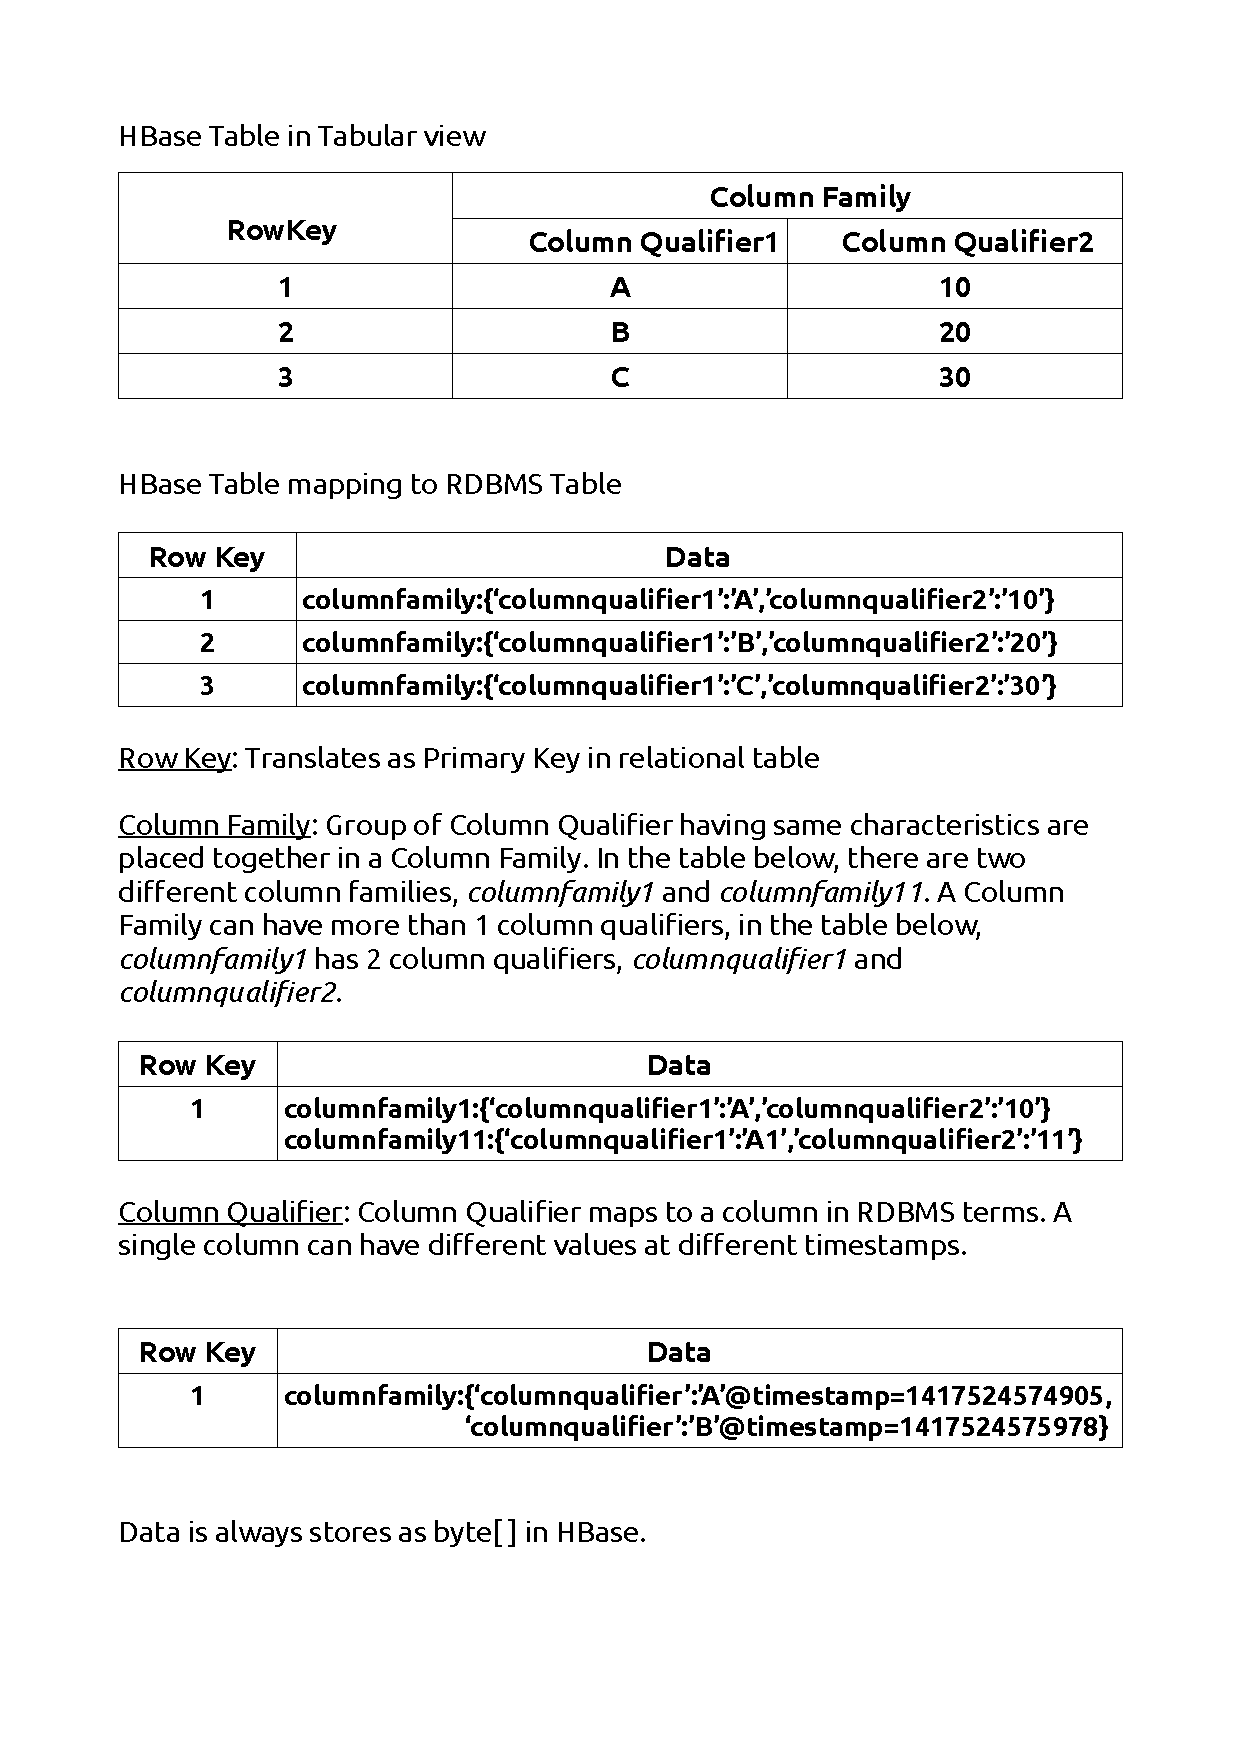
\includegraphics[width=\linewidth]{HBase}
% 	\caption{HBase}
% 	\label{fig:HBase}
% \end{figure}

\newpage
\subsection{HBase Architecture}
\label{HBase Architecture}

HBase architecture consists of three major components and three sub components. The major components are Master, Region server and zookeeper. The three sub components are Write-Ahead-Log(WAL), HFile and Memstore\cite{hbase:insights}. HBase architecture is based on Master-Slave architecture, where the Master is known as HMaster, is the master node and Region Servers are the slave nodes. Whenever the write request is sent, HMaster receives the request and forwards it to the respective Region Server\cite{hbase:insights}. 

\subsubsection{HMaster}
\label{hmaster}

HBase Master is mainly responsible for region assignments within the region servers and DDL operations like creating and deleting tables\cite{hbase:architecture}. Apart from these roles, HMaster is also responsible for assigning the regions and re-assigning of the regions for recovery or load balancing\cite{hbase:architecture}. HMaster also monitors all the instances of Region Servers in the cluster\cite{hbase:architecture} and mainly provides administrative operations.

\subsubsection{Region Servers}
\label{region serves}

Region servers are systems within HBase that acts like a data node\cite{hbase:insights}. When a HMaster receives a write request, it forwards the request to the Region Server. Region server can have multiple regions within it, and it directs the request to the specific region. Region servers are mainly responsible for handling data related operations and communication. Region servers handle the read/write request for all the regions within it. 
A Region Server runs on data node and it has four sub components as described below\cite{hbase:architecture}
\begin{description}
	\item[$\bullet$]  Write Ahead Log(WAL): Write Ahead Log is basically a log file. Region server adds each request to WAL first before sending that request to the appropriate region. It is mainly used for recovery in case of failure\cite{hbase:insights}. If the request is not written in the WAL file, there is a possibility of data loss in case of Region Server failure.
\end{description}

\begin{description}
	\item[$\bullet$]  BlockCache: BlockCache is the read cache that is used to store frequently read data\cite{hbase:insights}. When the cache is full, last read data is removed from the cache.
\end{description}

\begin{description}
	\item[$\bullet$] MemStore: MemStore is the write cache. All the new data that has not been written to the disk are stored in MemStore. It is mainly responsible for keeping tracks of all the logs for read and write operations to be performed for a specific Region Server\cite{hbase:architecture}. Each column family in a region has one MemStore\cite{hbase:insights}.
\end{description}

\begin{description}
	\item[$\bullet$] HFile: In HBase, column family is a collection of multiple HFiles. HFiles are used to store rows as keyValue pairs and are immutable and sorted\cite{hbase:insights}.
\end{description}

\subsubsection{Zookeeper}
\label{zookeeper}
Zookeeper an open source project under Apache Software Foundations, is a distributed software system that provides a infrastructure for synchronization across the clusters. It provides coordination between distributed processes across the cluster so that client receives consistent data. The architecture of Zookeeper is based on client-server model. The client acts as a node that make use of the service and server acts as a node that provides the service\cite{hbase:zookeeper}. Many Zookeeper servers can be collected together, that is known as $Zookeeper$ $ensemble$\cite{hbase:zookeeper}. Each server node of the zookeeper at a given time can handle large number of client connections. It is essential to know if the connection is alive, so the client node sends a ping request to the server it is connected to make sure it is connected and alive\cite{hbase:zookeeper}. The server, after receiving ping request, sends an acknowledgement to indicate that server is alive. If the client doesnot receive acknowledgement within a given specific time, then the client connects to another zookeeper server within a $Zookeeper$ $ensemble$ and the client session is transferred to the new zookeeper server\cite{hbase:zookeeper}.
\newline
HBase has a tight integration with Zookeeper. HBase uses Zookeeper as a distributed coordination service to facilitate synchronization between the servers in a cluster. HBase also uses Zookeeper to keep track of state of the servers, which servers are alive and available\cite{hbase:architecture}. Whenever a HBase instance is started, it automatically starts Zookeeper instance, as Zookeeper comes integrated with HBase\cite{hbase:insights}. Zookeeper is used to keep tracks of the number of regions servers available, and the data hold by each region servers. 
\newline

The figure below explains the HBase Architecture and its components.
\begin{figure}
	\centering
	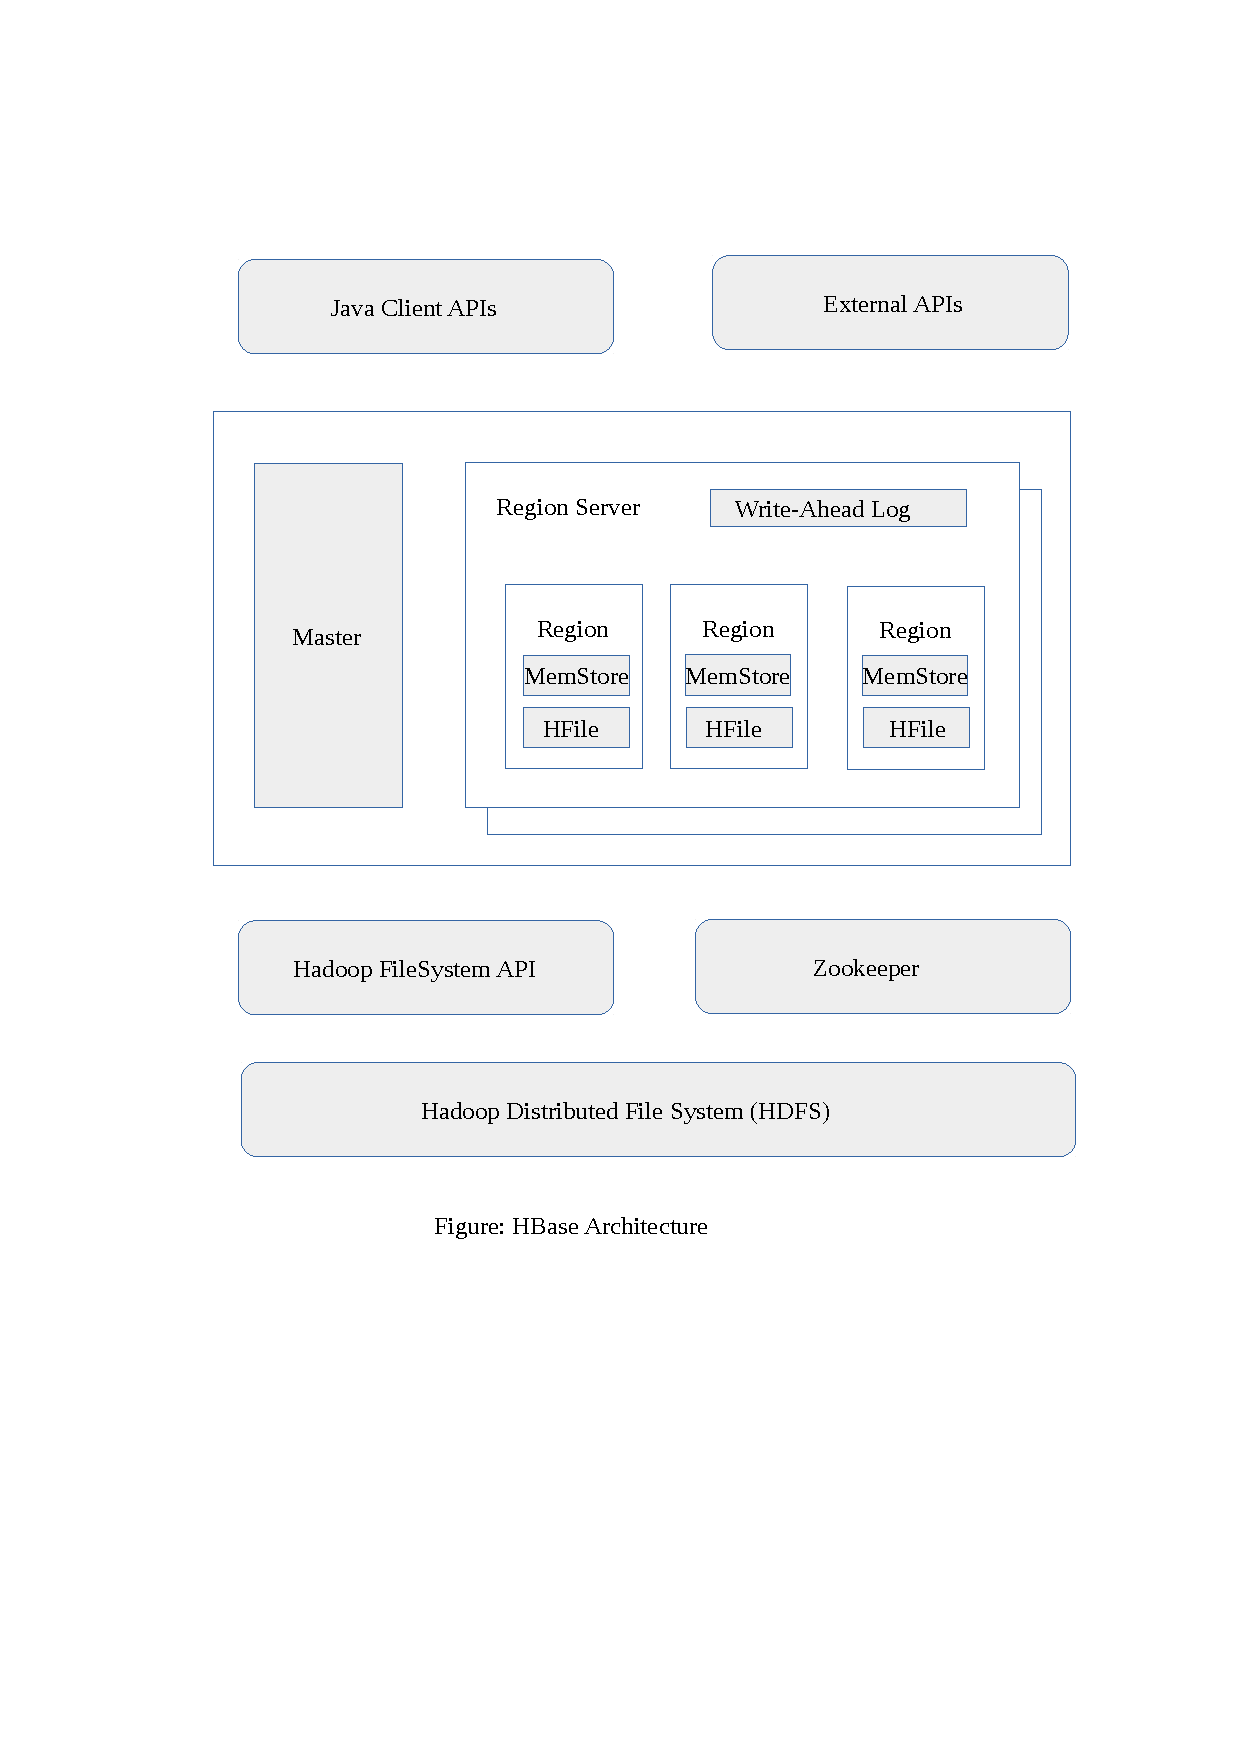
\includegraphics[width=\linewidth]{HBase_Architecture}
	\caption{HBase Architecture}
	\label{fig:hbasetable}
\end{figure}

\newpage
\section{Hadoop Distributed File System}
\label{Hadoop Distributed File System}

The Hadoop Distributed File System (HDFS) is an open source distributed file system developed for the Hadoop framework. HDFS is designed to store very large data sets and run on a commodity hardware. In HDFS, each files are divided into blocks of fixed size and are stored across multiple machines\cite{HDFS:architecture}. HDFS is also based on client-server architecture and each HDFS cluster consists of a single NameNode, also called as Master Node and multiple DataNodes, known as Slave nodes. All the metadata are stored in NameNode wheres the application data resides in DataNodes\cite{hadoop:architecture}.

\subsection{NameNode}
\label{NameNode}
NameNode is the master node of HDFS file system. NameNode is the centerpiece in the HDFS architecture and is responsible for keeping the directory tree of all the files in a system\cite{HDFS:namenodeanddatanode}. Namenode does not store any data of the files, it stores 
only the metadata like namespace information and block information of HDFS\cite{HDFS:namenodeanddatanode}, and the data are stored in Data nodes. NameNode maps files into the set of blocks, and maps those blocks to a data nodes and directs data nodes to execute I/O operations\cite{HDFS:namenodeanddatanode}. For example, when a client wants to locate a particular file, Namenode intercepts the request from the client and returns response by retrieving all the possible data nodes where the file resides. Since there is only one NameNode in the HDFS cluster, it is subjected to a single point of failure in HDFS Cluster. If a Namenode is down, all the running processes will terminate as a result of which the entire HDFS cluster goes offline\cite{HDFS:namenodeanddatanode}.  

\subsection{SecondaryNameNode}
\label{SecondaryNameNode}
As the name suggests, it is assumed that SecondaryNameNode is used as a backup node in case of single point of failure. From subsection \ref{NameNode}, we know that NameNode stores meta information like namespace and block information. All these informations are stored in main memory and also in the physical disc for persistence storage\cite{HDFS:secondarynamenode}. Whenever a NameNode is started, the snapshot of the file system is stored in fsimage file and logs of the changes made after NameNode is started is written in Edit logs. There might be an issue when edit logs become very large and hard to manage. So SecondaryNameNode is used as a checkpoint in the HDFS. It fetches the edit logs from the namenode in reqular interval and updates fsimage with edit logs.The recent fsimage is copied back to the NameNode\cite{HDFS:secondarynamenode}. Since SecondaryNameNode cannot process the metadata to the disc\cite{HDFS:architecture}, it can not be used as a substitution to the NameNode.

\subsection{DataNode}
\label{DataNode}
DataNodes are the slave nodes in the HDFS file system. There can be one or many data nodes in a HDFS cluster. The data nodes are responsible for storing the files in a HDFS cluster. When the DataNode is started, it sends information about all the files and blocks stored in that node to the NameNode\cite{HDFS:datanode}. DataNode, likewise NameNode, is also expected to fail at some point. But this doesnot let the HDFS cluster to go offline. In such scenario, NameNode will replicate the blocks and files managed by failed DataNode\cite{HDFS:namenodeanddatanode}. 


\section{Coprocessor}
\label{sec:coprocessor}

HBase Coprocessor framework provides a library to run user code in the HBase Region Server. The advantage of this framework is that it decreases the communication overhead of transferring the data from HBase region server to the client, thus improving the performance by allowing the real computation to happen in the HBase region server\cite{coprocessor:coprocessor}. There are two types of coprocessor, Observer coprocessor  which acts more like relational database triggers and Endpoint coprocessor that resembles stored procedures of RDBMS\cite{coprocessor:types} 


\subsection{Observer coprocessor}
\label{sec:observercoprocessor}
Observer coprocessor as stated earlier, is more like database triggers that executes our code when certain events occur. In the figure below, we first try to explain a simple life cycle of put() operation as an example\cite{coprocessor:detail}. Observer coprocessor resides between the client and the HMaster. Observer coprocessor can be triggered after every get(), put() or delete() command. The CoprocessorHost class is responsible for observer registration and execution\cite{coprocessor:detail}.  During the life cycle of events, Observer coprocessor allows us to hook triggers in two stages. The first one is before the occurrence of the event and the other is after the completion of the event. For example, if we want to perform some computations before the occurrence of put event, we can use prePut() method to perform our custom computation. Then the life cycle of put event starts and after the life cycle of put event is completed, we can use postPut() method to perform custom computation. In the figure below, we try to explain the lifecycle of observer coprocessor when a put event is fired\cite{coprocessor:detail}.
\newline
There are four types of Observer Interfaces provided as of HBase version 1.1.3\cite{hbase:essential}.

\begin{enumerate}
    
\item RegionObserver: RegionObserver runs on all the Region of a HBase table. RegionObserver provides hook for data manipulation for events like put(), get() add delete() events. All the data manipulations are done with pre-hook and post hook\cite{hbase:essential} such as pre and post observers. For instance, preGetOp() and postGetOp() provides hook for manipulating get request. 

\item RegionServerObserver: Likewise in RegionObserver, RegionServerObserver provides a hook for data manipulation for events like merge, commits and rollback. All the data manipulation are done with pre-hook and post hook such as preMerge() and postMerge(). 

\item WALObserver: WALObserver interface provides a hook for Write-Ahead-Log(WAL)\cite{hbase:essential} related operations. This interface provides only preWALWrite() which is triggered before WALEdit is written to Write-Ahead-Log and postWALWrite() which is triggered after WALEdit is written to a Write-Ahead-Log.

\item MasterObserver: MasterObserver Interface provides a hook for data manipulation for DDL events such as table creation, table deletion or table modification\cite{cloudera:instandupg}. For instance, if the secondary indexes need to be deleted when primary table is deleted, we can use postDeleteTable(). The MasterObserver runs on the master node.

\end{enumerate}

\begin{figure}
    \centering
    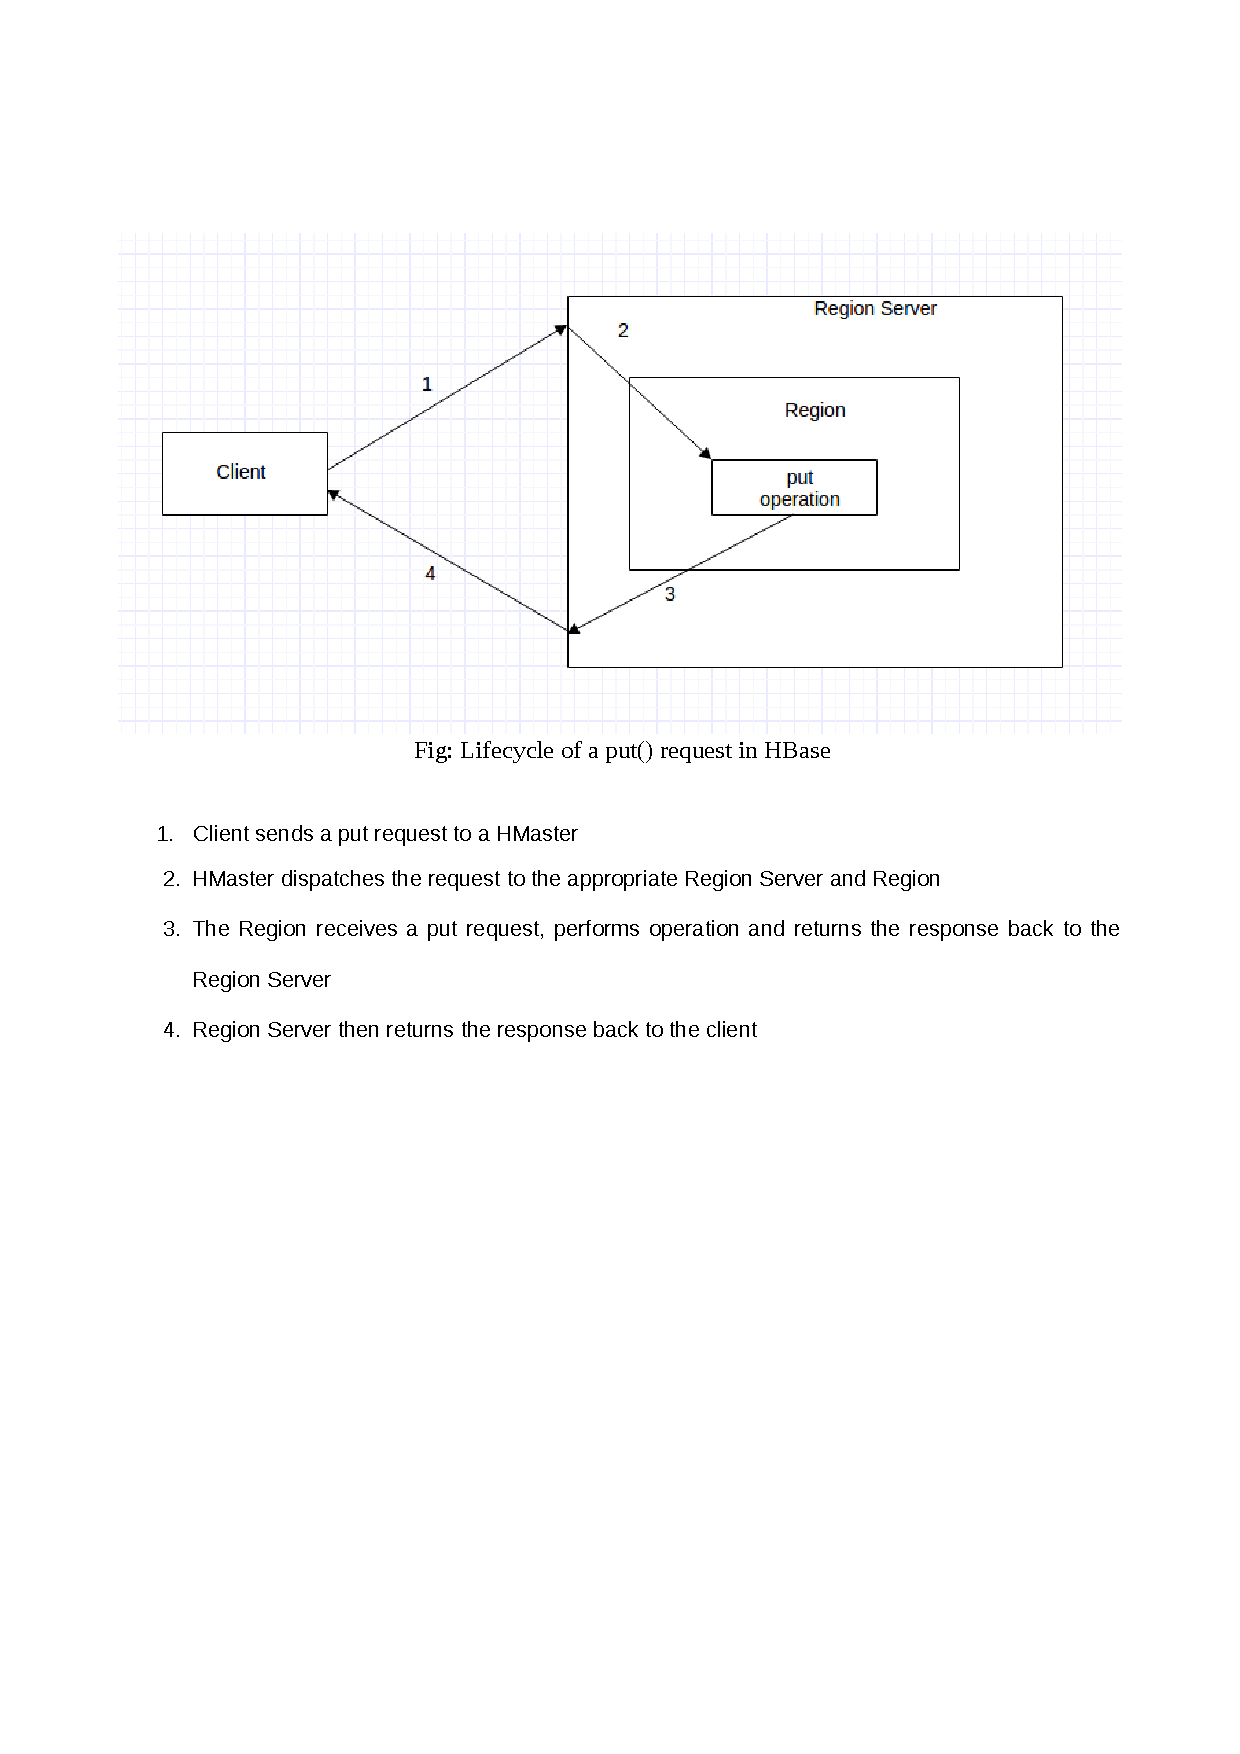
\includegraphics[width=\linewidth]{PutRequestLifeCycle}
    \caption{Life cycle of put request}
    
\end{figure}

In the figure below, We can see the life-cycle of a put request with observer coprocessor implemented.

\begin{figure}
    \centering
    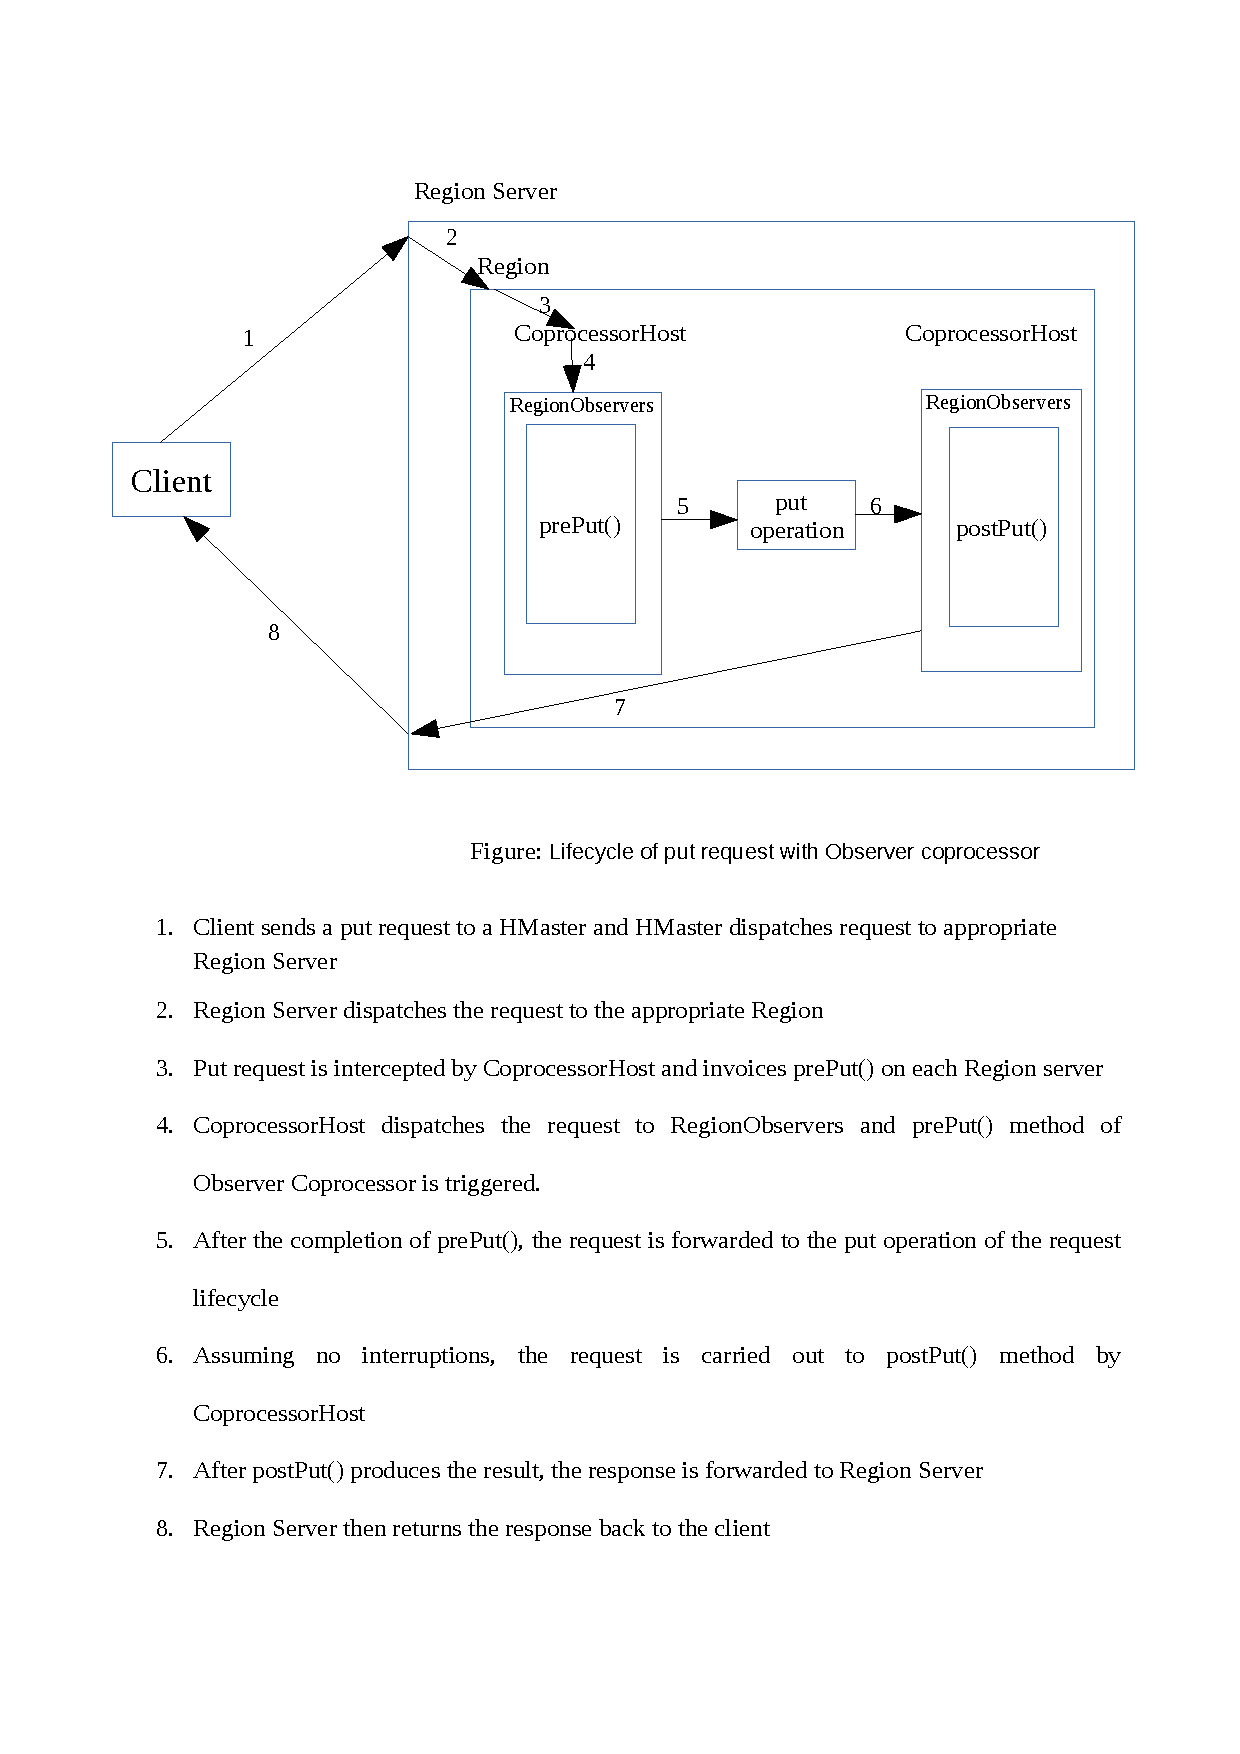
\includegraphics[width=\linewidth]{PutRequestWithObserverCoprocessor}
    \caption{Life cycle of put request with observer coprocessor}
    
\end{figure}

\newpage
\subsection{Endpoint coprocessor}

Endpoint coprocessor is similar to the Stored Procedures in RDBMS. This type of coprocessor is more useful in the scenario where the computation is needed for the whole table and are not provided by observer coprocessor\cite{hbase:coprocessors}. Invoking the endpoint coprocessor is similar to invoking any other commands in HBase from the client\textquotesingle s point of view but the result is based on the code that defines the coprocessor\cite{coprocessor:detail}. The figure below explains the Aggregation example\cite{coprocessor:detail}.

\begin{figure}
    \centering
    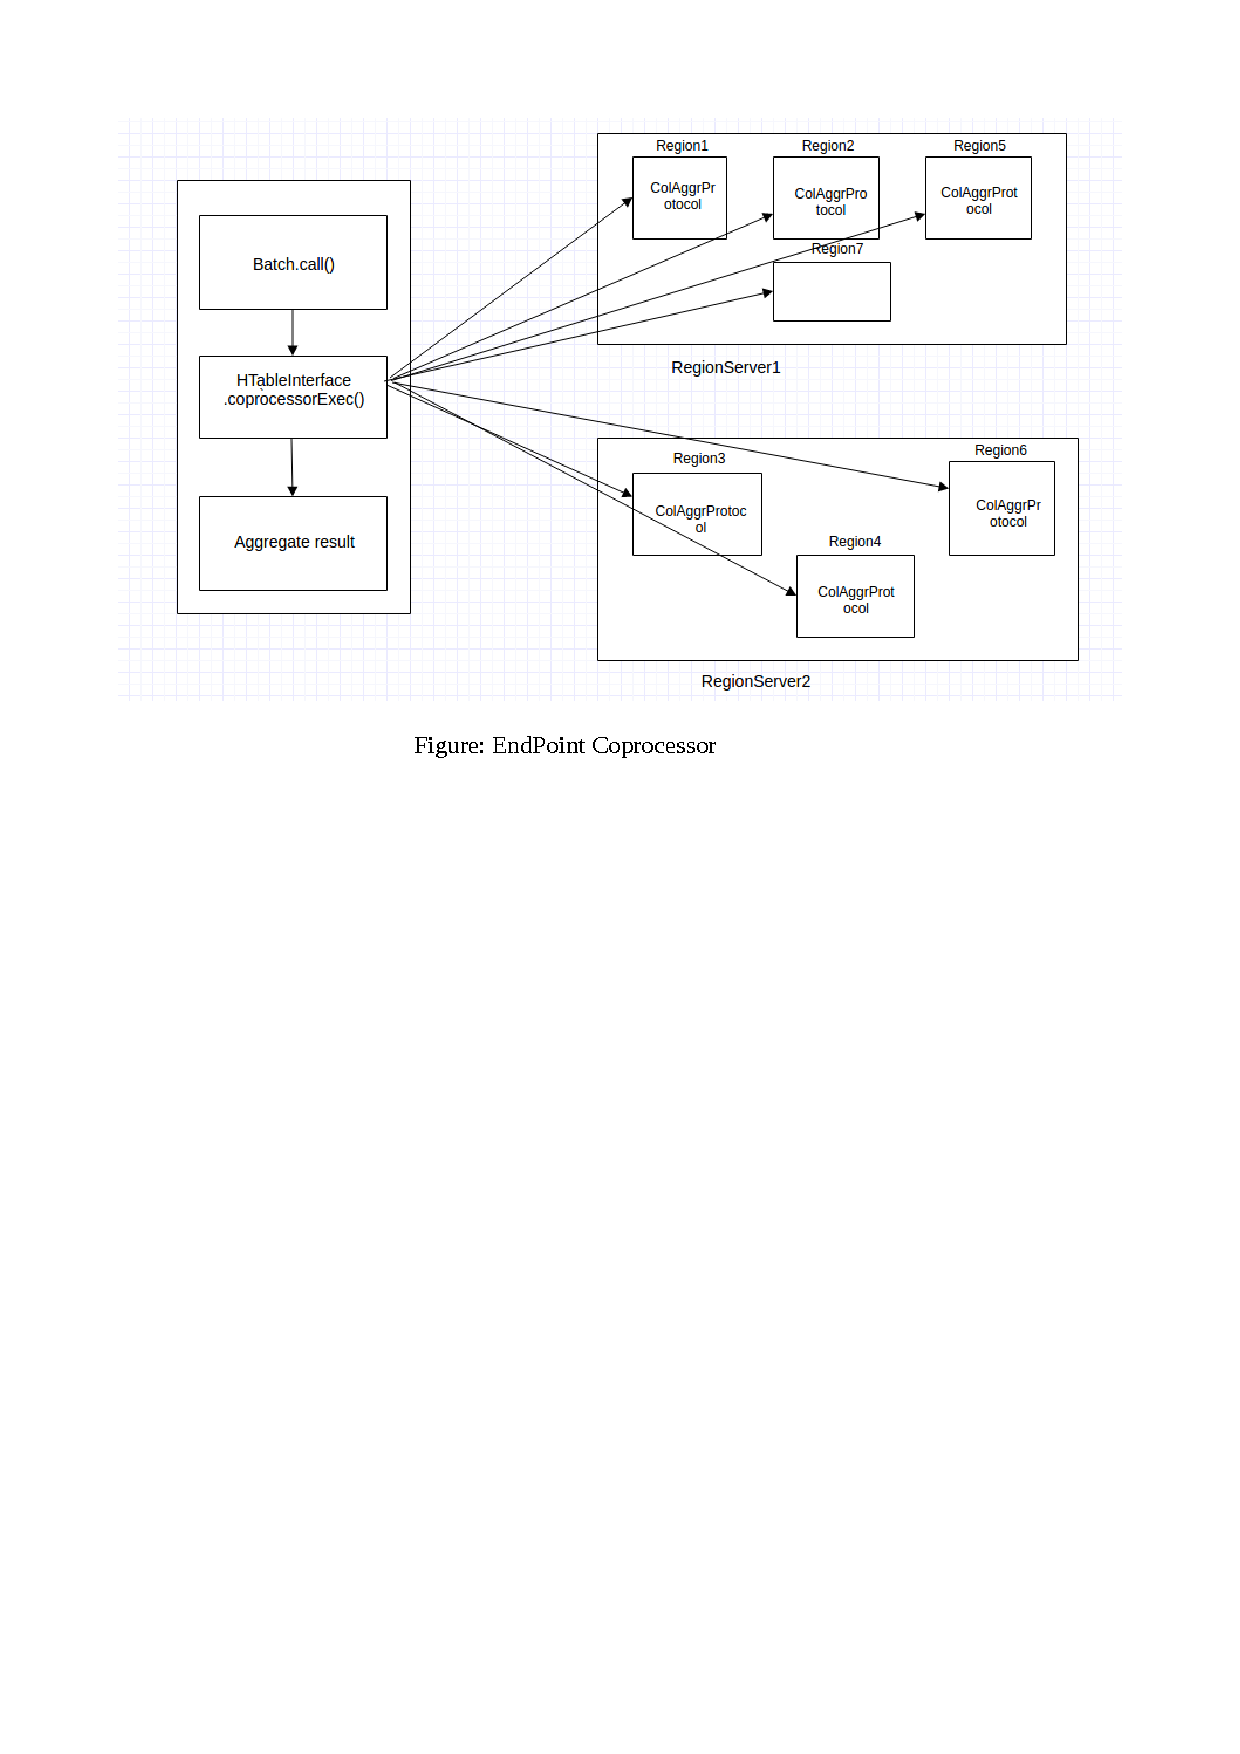
\includegraphics[width=\linewidth]{EndPointCoprocessor}
    \caption{EndPoint Coprocessor}
    
\end{figure}

When a request is invoked from a client, an instance of Batch.call() encapsulates the request invocation and the request is forwarded to coprocessorExec() method of HTableInterface. Then the coprocessorExec() handles the request invocation and distributes the request to all the Regions of the RegionServer. Assuming that no interruptions occurs and all the requests are completed, the results is then returned to client and aggregated\cite{coprocessor:detail}.


\chapter{Related Work}
\label{chap:relatedwork}
In this chapter, we will discuss the existing research that have been made to maintain consistency between base table and view table.

\section{Foundations}
\label{Foundations}
In the early 90's when relational database systems were popular and widely used, several research were conducted to optimize the query processing time. The idea of using materialized view when-ever possible to evaluate a query for the benefit of improved query processing was proposed more than a decade ago\cite{maintenance:optimizingqueries}. Several methods have been proposed for incremental view maintenance in the past\cite{blakeley:efficiently, gupta:maintaining, agrawal:efficient}.

In\cite{incremental:materializedviews}, the researchers have investigated the problem of incremental maintenance of a materialized view. The researchers in paper\cite{incremental:materializedviews} have proposed an auxiliary relations to reduce the cost of view maintenance. They proposed a view that can be represented by an operator tree\cite{database:concepts} where leaf nodes represented database relations and non-leaf nodes represented relational algebraic operations. An auxiliary relation was maintained for each node, and the key of auxiliary relations is a foreign key that matched the primary key of each relation, thus maintaining referential integrity between auxiliary relations and base relations\cite{database:concepts}. These auxiliary relations are also changed in response to the base relations changes.

In paper \cite{incrementalmaintenance:materializedviews}, the researchers have demonstrated an algorithm for incremental view maintenance based on graph-based data model and query language Lorel developed at Stanford. Their algorithm produces a set of queries that computes the changes to be made to the view table based on the changes to the base table. Researchers proposed a view specification extension to Lorel query language\cite{incrementalmaintenance:materializedviews} that introduced two objects in the view model: $select-from-where$ and $with$. The $select-from-where$ model specified the primary objects imported to the view and the later one $with$ model specified paths from primary objects to the adjunct objects\cite{incrementalmaintenance:materializedviews}. Their algorithm generates a set of maintenance statements for a given view and a database object, evaluates the updates on the database to generate new set of view updates and finally installs the updates in the view\cite{incrementalmaintenance:materializedviews}.

In paper \cite{maintenance:materializedviews}, the researchers have classified four dimensions along which the view maintenance problems has to be studied. 
\begin{itemize}
	\item Information Dimension: This dimension deals with the amount of information available for view maintenance. Some of the prior information regarding integrity constraints and keys, access to materialized views has to be known before developing an algorithm for incremental maintenance.
	
	\item Modification Dimension: This dimension deals with problem statements related to modification of a system. Some prior knowledge has to be acquired such as what modifications can be handled by a view maintenance algorithm, how update tuples are handled, are they handled directly or are they modeled as deletion followed by insertion tuples.
	
	\item Language Dimension: This dimension addresses problem related with select-project-join query, i.e. does view consists of entire SQL or subset of SQL. It also defines problem statements whether SQL statement can use aggregation function, recursion function or closure. 
	
	\item Instance Dimension: This dimension addresses problems related to instance of database such as if view maintenance algorithm works for all the instances of the database for just for some particular instances. 

\end{itemize}

In paper \cite{maintenance:optimizingqueries}, researchers found that blind applications using materialized views resulted in much worse results than application not using materialized views. The research found out that using materialized views to optimize query performance depends on the query and statistical properties of the database\cite{maintenance:optimizingqueries}. The statistical properties of the database are time-varying and also most of the times, queries are generated using tools, $cost-based$ decision has to be taken whether to use or not to use materialized views to answer a given query in the database\cite{maintenance:optimizingqueries}. There might also be cases where more than one materialized view can be relevant for a given query, so in this case, incorrect alternatives has to be avoided to gain performance advantage. Researchers in paper \cite{maintenance:optimizingqueries} have proposed an algorithm for optimizing materialized views in three steps. In the first step, the query is translated into canonical unfolded form, i.e. system that supports views. In the second step, they identify possible ways to generate one or more materialized views for a given query. In the third step, they use efficient join enumeration algorithm to predict the cost of each alternative formulations and the path with least cost is selected\cite{maintenance:optimizingqueries}.

\chapter{Failure Detection}
\label{Failure Detection}
Many of the large scale distributed systems are often subjected to Failure. Likewise, HBase is also subjected to failure. However, like other large scale distributed systems, HBase also guarantees availability and reliability in case of node failures. In such a large scale distributed systems where there are hundred's of nodes, manually detecting failure nodes and replacing them with new nodes is nearly impossible. In our design, we mainly focus on master failure and region server failure.

\section{Master Failure}
\label{Master Failure}
The primary job of HBase Master is to monitor all the available Region Server Instances in the cluster. In order for HBase to be up and running, HBase Master should always be available. HMaster, with no exception, is subjected to failure at some point of time. If no master is running at some point of time, the entire system goes offline. So to avoid such failure, HBase always has a single running master and multiple backup masters running at the same time. The master and backup masters are managed by Zookeeper. When the running master goes offline, Zookeeper appoints a new master from the available backup masters.

\section{Region Server Failure}
\label{Region Server Failure}
HBase Master monitors all the available Region Servers in a cluster. There can be multiple ways in which the region servers can go offline. When a particular region server fails, all the regions within that region server also go offline. Zookeeper then finds out about the failed region server when it looses heart beat with it. After the failed region server is detected, Zookeeper notifies HMaster about the failed Region Server. HMaster then reassigns all the regions from failed region server to the active region server. Now HMaster has to recover memstore edits from the failed region server. The Write-Ahead-Log(WAL) of the failed region server is split into separate files and stored in new region server's data node by HMaster.

\newpage
\chapter{Implementation}
\label{Implementation}
In this section, we will first discuss the prerequisite of implementation and then the proposed method for our research.

\section{Prerequisite}
Before we begin with our implementation of the coprocessor, there are few steps to load coprocessor into our HBase table. The coprocessor can be loaded to the base tables in two ways: statically and dynamically\cite{loading:coprocessors}. 

\subsection{Static Loading of coprocessor}
We have to define coprocessor properties in a $hbase$-$site.xml$ file inside a \textless property\textgreater \space element followed by \textless name\textgreater \space and a \textless value\textgreater \space sub element. The \textless name\textgreater \space sub element should have one of the followings\cite{hbase:site}:

\begin{enumerate}
    \item hbase.coprocessor.region.classes for RegionObservers and Endpoints coprocessor
    \item hbase.coprocessor.wal.classes for WALObservers
    \item hbase.coprocessor.master.classes for MasterObservers
    
\end{enumerate}

The \textless value\textgreater \space sub-element should contain the full path of the coprocessor implementation class. A typical example for static loading of coprocessor looks as,\newline \newline \textless property\textgreater \newline
\textless name\textgreater hbase.coprocessor.region.classes\textless /name\textgreater \newline
\textless value\textgreater \texttt{org.apache.hbase.HBase\_coprocessor.HBaseCoprocessor}\textless /value\textgreater \newline
\textless /property\textgreater \newline

 If we have multiple classes, then the path in \textless value\textgreater \space sub-element should be comma separated. In this setup, the framework will attempt to load all the configured classes, so we have to create a jar with dependencies, for all the classes and place the location of the jar to HBase classpath. For that, we have to export /path/to/jar in $hbase$-$env.sh$ file. A typical example for exporting classpath is given below, \newline \newline
 export \texttt{HBASE\_CLASSPATH}='/path/to/jar' \newline
 
Now if HBase is restarted without any errors, we have managed to load system coprocessor successfully. 

\subsection{Static Unloading of coprocesssor}
\begin{enumerate}
    \item Delete entry from $hbase$-$site.xml$
    \item Delete entry for $hbase$-$env.sh$
    \item Restart HBase
\end{enumerate}

\subsection{Dynamic Loading of coprocessor}
In this approach, rather than loading coprocessor to all the tables in a Region, the coprocessor is loaded to specific tables of the region. There are two implementations of loading coprocessor dynamically, from HBase shell or using Java API\cite{hbase:site}.

\subsubsection{Using HBase shell}
\begin{enumerate}
	\item disable table \newline
			\space \space hbase\textgreater disable '\textless \texttt{table\_name}\textgreater'
	\item load coprocessor using the following command \newline
	alter '\textless \texttt{table\_name}\textgreater', \newline 
	METHOD =\textgreater '\textless \texttt{table\_att}\textgreater', 'coprocessor' =\textgreater '/file/to/path\text{\textbar}\newline/source/path/to/impementation/class\text{\textbar}1001\text{\textbar}'
	\newline \newline
	A typical example looks like,\newline \newline
	alter 'BaseTableA', METHOD =\textgreater '\texttt{table\_att}', 'coprocessor' =\textgreater 'file:///home/saroj-gautam/Documents/HBase-coprocessor-0.0.1-SNAPSHOT-jar-with-dependencies.jar\text{\textbar}\texttt \newline {org.apache.hbase.HBase\_coprocessor.HBaseCoprocessor}\text{\textbar}1001\text{\textbar}'
	
	\item enable table \newline
	See if coprocessor is loaded successfully. We can see it by seeing the table properties. \newline 
	hbase\textgreater describe '\textless \texttt{table\_name}\textgreater \space should list the coprocessor under \texttt{TABLE\_ATTRIBUTES.} \newline

\end{enumerate}

In the above scenario, the coprocessor tries to read class information from \texttt{table\_att} property. There are certain arguments separated by pipe (\text{\textbar}). The first argument in the value is the file path to the jar file that contains the implementation class. The second argument contains the full classname of the implemented coprocessor. The last argument represents the execution sequence of registered observers. If this field is left blank, the framework will itself assign a default priority value\cite{hbase:site}.

\subsubsection{Using Java API}
Prior to HBase version 0.96, the coprocessors were loaded in a different way. After HBase version 0.96 and newer, HTableDescriptor class provides addCoprocessor() method that helps to load coprocessor in an easier way. A code snippet\cite{loading:coprocessors} below will give us a basic insight of how coprocessor is loaded dynamically from Java API in older versions and newer versions of HBase.
\newline \newline
\textbf{Older than 0.96} \newline
\lstset{language=Java}
\begin{lstlisting}
String path = "/path/to/jar"
admin.disableTable(<table_name>)
hTableDescriptor.setValue("COPROCESSOR$1", path + "|"
    + RegionObserverExample.class.getCanonicalName() + "|"
    + Coprocessor.PRIORITY_USER);
admin.enableTable(<table_name>)
\end{lstlisting}

\textbf{0.96 or newer} \newline
\lstset{language=Java}
\begin{lstlisting}
String path = "/path/to/jar"
admin.disableTable(<table_name>)
hTableDescriptor.addCoprocessor(<class_name>.class.getCanonicalName(),
             path, Coprocessor.PRIORITY_USER, null);
admin.enableTable(<table_name>)
\end{lstlisting}

\subsection{Dynamic Unloading of coprocessor}
Dynamic unloading of coprocessor can also be done in two ways, from shell and from Java API. 

\subsubsection{Using HBase shell}
\begin{enumerate}
    \item disable table
    hbase\textgreater disable '\textless \texttt{table\_name}\textgreater'
    \item alter table, remove coprocessor
    hbase\textgreater alter '\textless \texttt{table\_name}\textgreater', \newline
    METHOD =\textgreater '\texttt{table\_att\_unset}', NAME=\textgreater 'coprocessor\$1' =\textgreater
    \item enable table
    hbase\textgreater enable '\textless \texttt{table\_name}\textgreater'
     
\end{enumerate}

\subsubsection{Using Java API}
Using Java API, in the newer version we can use removeCoprocessor() method provided by HTableDescriptor class and in the older version, we can use setValue() to unload coprocessor.

\section{Proposed Method}
In this section, we will explain about the algorithms we've implemented to maintain incrementally materialized views for 
\begin{enumerate}
    \item Aggregation
    \item Join and Aggregation
    \item Join and Selection
\end{enumerate}

One of the most important features in our implementation is the introduction of intermediate table. We have introduced an intermediate table in order to restrict scanning of the entire base table for a simple get, put or delete operation. Scanning billions of rows for such operations can be expensive in terms of processing power and CPU usage. When an update/delete operation happens in the base table, updates in view table are calculated on the basis of updates in the intermediate table.

\subsection{Creation of an Intermediate table}
\label{subsec:intermediatetable}

We create an intermediate table in such a way that we have a single row for all the unique keys in the base table. This architecture restricts scanning the entire base table for any update or delete operation. Instead, we only scan particular row containing the key for which an update or delete operation is triggered. In our implement, there are two ways in which we create our intermediate table.

\subsubsection{Single Base Table}
\label{Single Base Table}
In this scenario, we have one base table and we have to create an intermediate table from the base table. The $columnFamily$ of the base table becomes $columnFamily$ in the intermediate table. The unique values of column $Key$ of the base table becomes $rowKey$ in the intermediate table and $rowKey$ of the base table becomes $column$ in the intermediate table. Once we create our intermediate table, we put the values from the base table into the intermediate table. Fig(a) in \ref{Intermediate Table} shows a graphical transformation of a single base table into an intermediate table. Now for any update or delete operations for a particular Key/Value in the base table, only a single row for that particular Key is updated in an intermediate table. This implementation restricts scanning of the whole base table for a single update/delete operation.

\subsubsection{Two Base Tables}
\label{Two Base Tables}
In this scenario, we have two base tables and we have to create an intermediate table from the two base tables. The both $columnFamilies$ of base tables are merged together into two $columnFamilies$ in the intermediate table. The unique values of column $Key$ of both base table becomes $rowKey$ in the intermediate table and $rowKey$ of the base table becomes $column$ in the intermediate table. Once we create an intermediate table from two base tables as described, we put values from both the base tables into the intermediate table. Fig(b) in \ref{Intermediate Table} shows a graphical transformation of a two base tables into an intermediate table. Now for any update or delete operations for a particular Key/Value in the base tables, only a single row for that particular Key is updated in an intermediate table. This implementation restricts scanning of the whole base table for a single update/delete operation.

\subsection{Creation of View Table}
A view table contains resultset of a query on the base table. In our implementation, view table is created on the basis of an intermediate table. Once we have our intermediate table, we apply certain algorithms on the intermediate table and create view table. Once we have our view table, our task is to maintain consistency between base table and view table. If any operation changes the state of base table, we reflect those changes in intermediate table and view table. The algorithm we've implemented maintains consistency incrementally, not re-computing view table for every changes in the base table. We will discuss our approach of this incremental maintenance in the sections below.

\begin{figure}
    \centering
    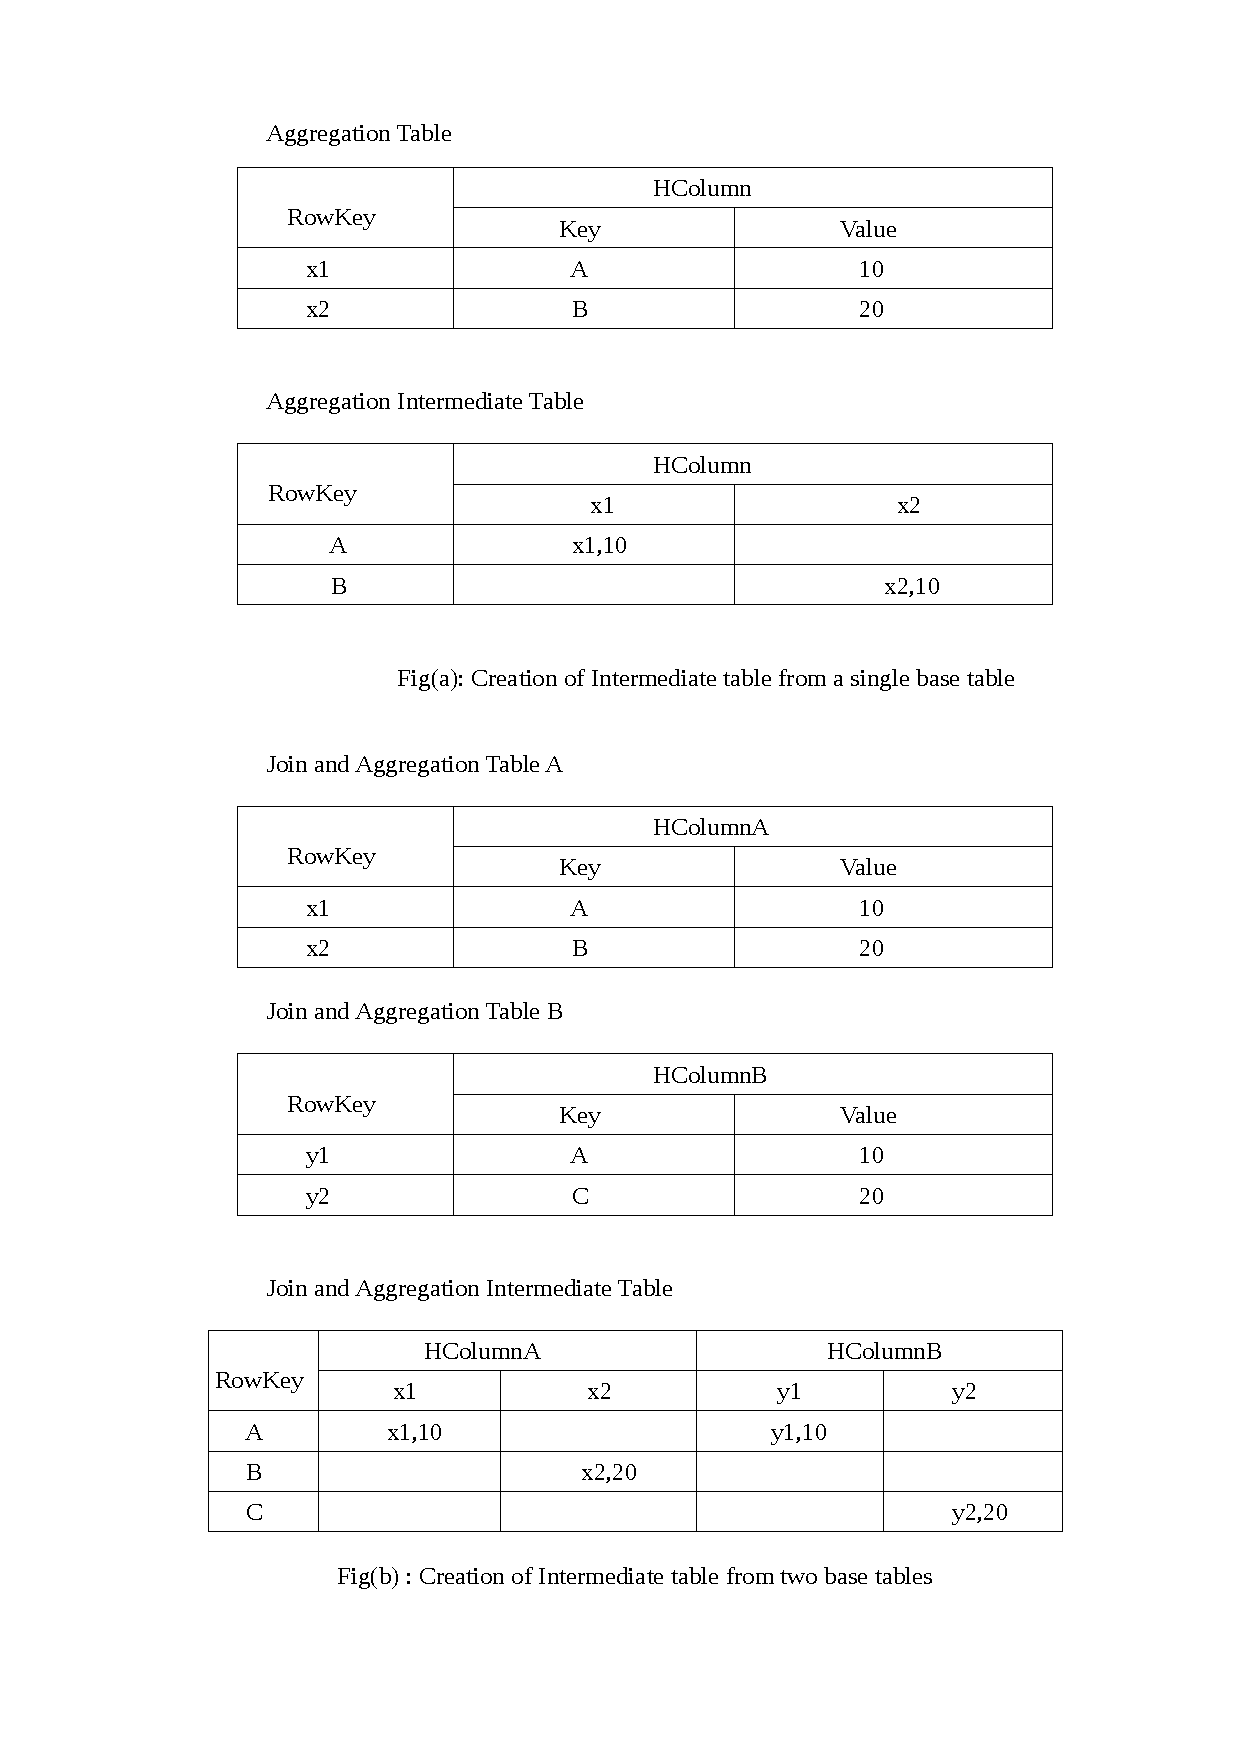
\includegraphics[width=\linewidth]{IntermediateTable}
    \caption{Creation of an Intermediate Table}
    \label{Intermediate Table}
    
\end{figure}

\newpage
\subsection{Aggregation}
\label{sec:aggregationImpl}

For Aggregation view type, we have a single base table with multiple key,value pairs. We create an intermediate table from a single base table as described in subsection \ref{subsec:intermediatetable}. The view table for Aggregation basically stores the result of aggregation functions namely $Sum$, $Count$, $Min$ and $Max$. These aggregation functions are carried out based on $Key$ of the base table. In this section we describe how we can maintain consistency incrementally between base table and view table. 

%In our implementation, we've implemented basic aggregation functions like sum, count, min and max. All these operations are carried out based on a particular key. The base table contains key,value pairs. We construct an intermediate table from the base table. The reason behind constructing an intermediate table is to restrict scanning of the whole base table for an update/delete trigger for a particular key in a base table. We take the unique keys and map them as a row key in the intermediate table, and accordingly the values are plotted. Once all the values are plotted in the intermediate table, we then construct view table. The view table contains aggregate functions like Sum, Count, Min and Max for each row Key i.e. for each unique keys of the base table. 

%The figure below explains how we map base table to a view table.

%\begin{figure}
%    \centering
%    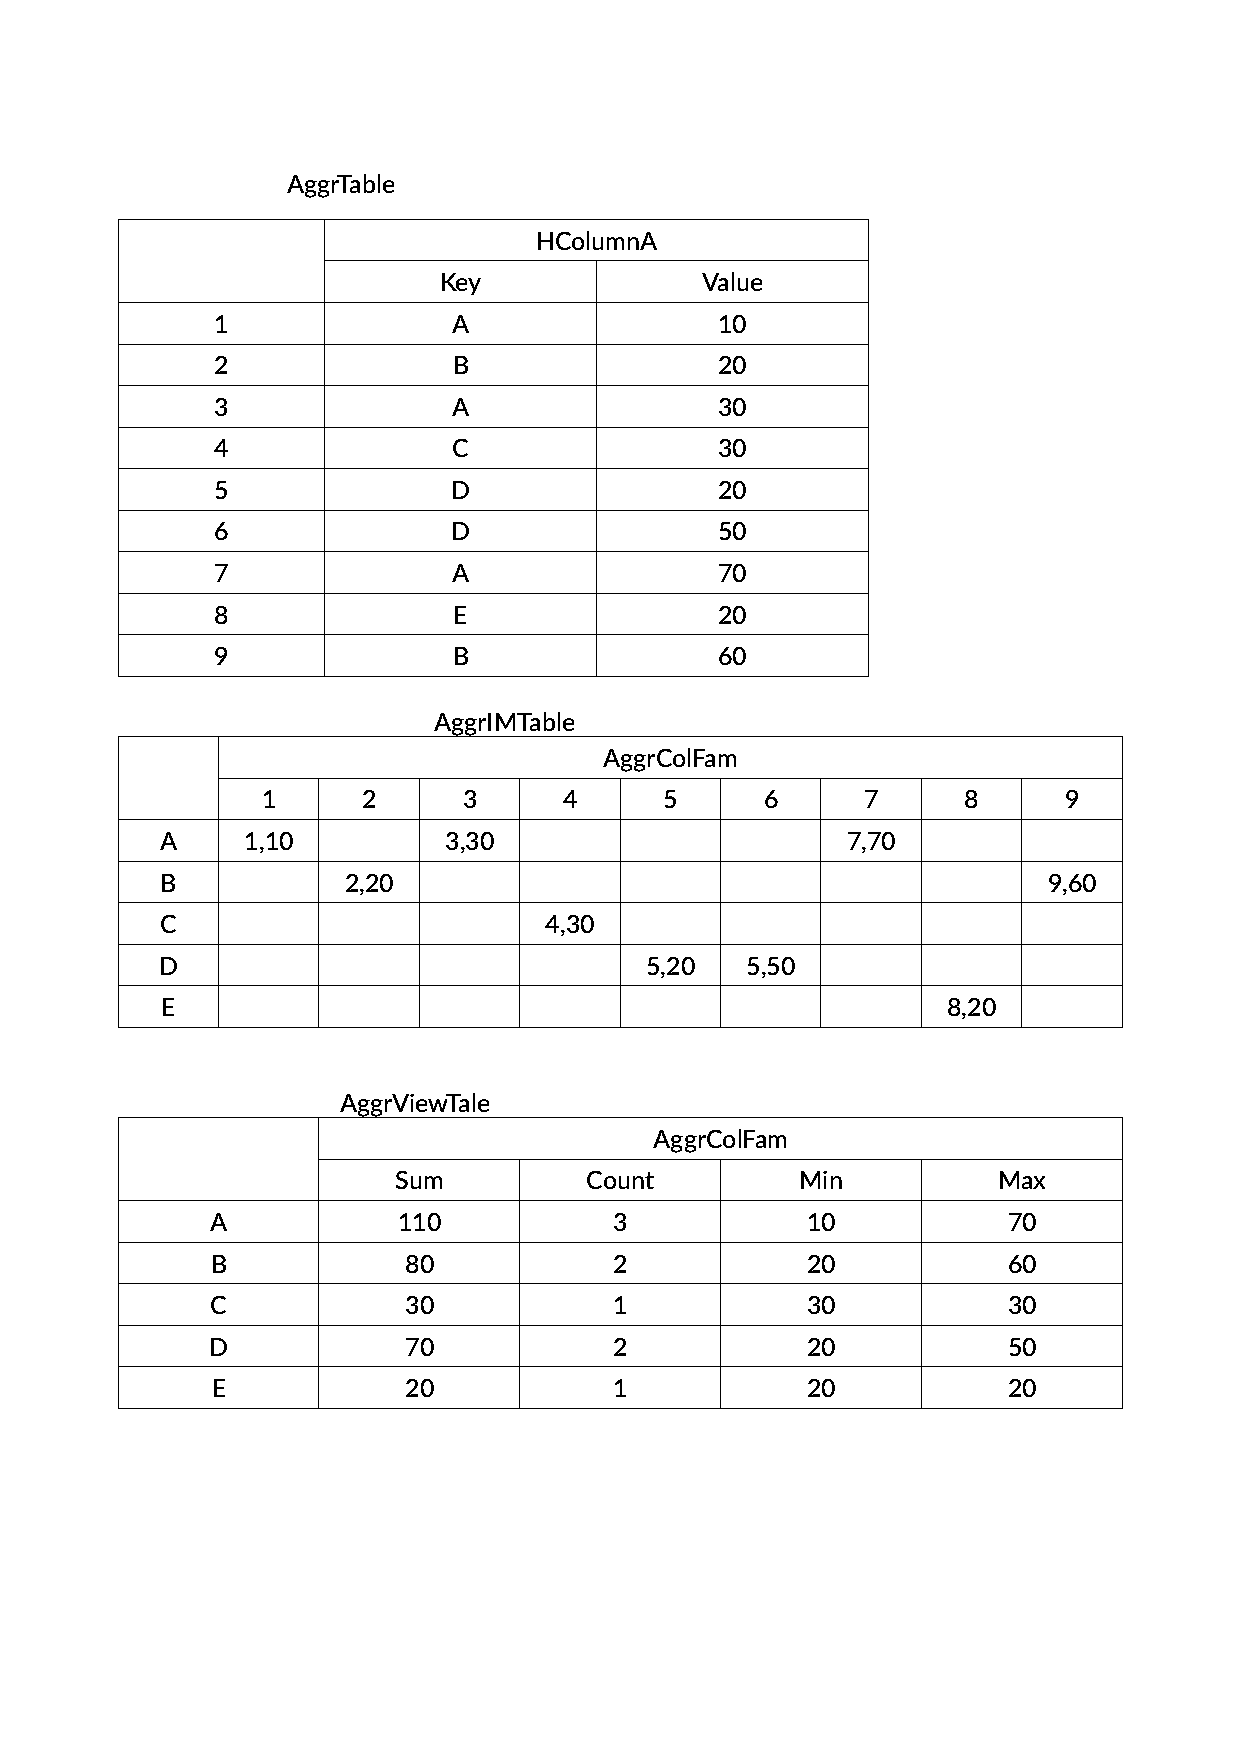
\includegraphics[width=\linewidth]{Aggregation}
%    \caption{Aggregation}
%    \label{sec:aggregation}
    
%\end{figure}
%\newpage

Once we have a base table, an intermediate table, a view table and coprocessor successfully loaded on our base table, we are ready to go ahead with our implementation. There are certain scenarios where coprocessor is triggered for an update and delete operations.

\begin{enumerate}
    \item New row is inserted
    \item Existing value of a row is updated
    \item Existing key of a row is updated
    \item Existing row is deleted
\end{enumerate}

\subsubsection{New row is inserted}
When a client issues an insert operation to insert a new key,value pair on the base table, we have to insert that key,value pair in our intermediate table and our view table has to be updated accordingly. The view table stores result of aggregation functions and the changes in the view table has to be updated incrementally. Using prePut() and postPut() triggers from observer coprocessor, we perform all the required operations.

As we have already discussed put() request life cycle in \ref{sec:observercoprocessor}, before the key,value is inserted, we catch the request using prePut() method provided by the observer coprocessor. In the prePut() method, we verify the inputs and check if new row is inserted or existing row is updated. After we verify that new row is inserted, we let the request to insert new key,value pair into the base table. After new key,value pair is inserted into the base table, we again catch the request in postPut() method. In postPut() method, we put new key,value pair in the intermediate table. Once the intermediate table has been updated, we need to update all the aggregation functions in the view table. We create a list and put all the key,value pairs for that particular rowKey of the intermediate table. From the list we update our aggregation functions and then update the result on the view table. The figure \ref{sec:newrowinsertagggregation} explains the scenario when a new row is inserted. The left side tables are the default tables and right side tables explain the behavior when a new row is inserted. The text displayed in red marks the changes that are happening on base table, intermediate table and  the view table. 
\begin{figure}
    \centering
    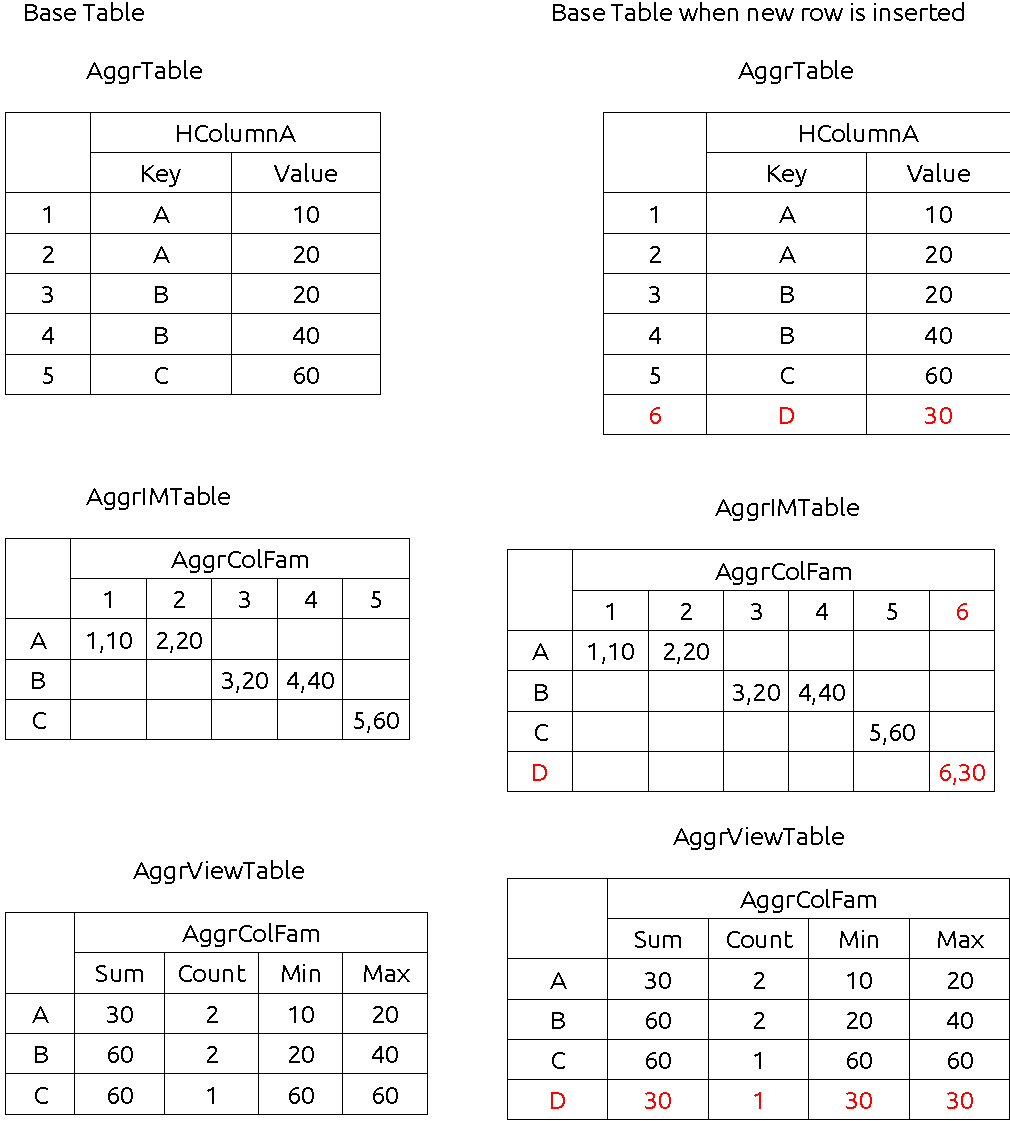
\includegraphics[width=\linewidth]{NewRowInsertAggr}
    \caption{New row insert}
    \label{sec:newrowinsertagggregation}
    
\end{figure}

\newpage
\subsubsection{Existing value of a row is updated}
Whenever an existing value of a key is updated, the base table is updated accordingly. Before the base table is updated, we catch the request via prePut() method of observer coprocessor. In the prePut() method, we get the key,value for which the value is going to be updated and also we verify if the value is being updated or the key is being updated. After we verify that value is updated, then we release the request and the value is updated in the base table. After the insertion, we catch the request via postPut() method of observer coprocessor, and then plot the updated value in our intermediate table for particular row key. Since we already have the row key, we only need to can that particular row, instead of scanning the whole intermediate table. This saves a lot of execution time and processing power. Once we plot updated value in the intermediate table, we then calculate aggregation functions for that particular row key and then update our view table accordingly. Now we need to update aggregation functions in the view table. We create a list and put all the key,value pairs for that particular rowKey of the intermediate table. From the list we update our aggregation functions and then update the result on the view table. The figure \ref{sec:updatevalueforexistingkey} explains the process in more detail. The updated value is marked in red on the right table, and also from the figure, we can see that we only iterate over a particular row key instead of scanning the whole base table and view table.

\begin{figure}
    \centering
    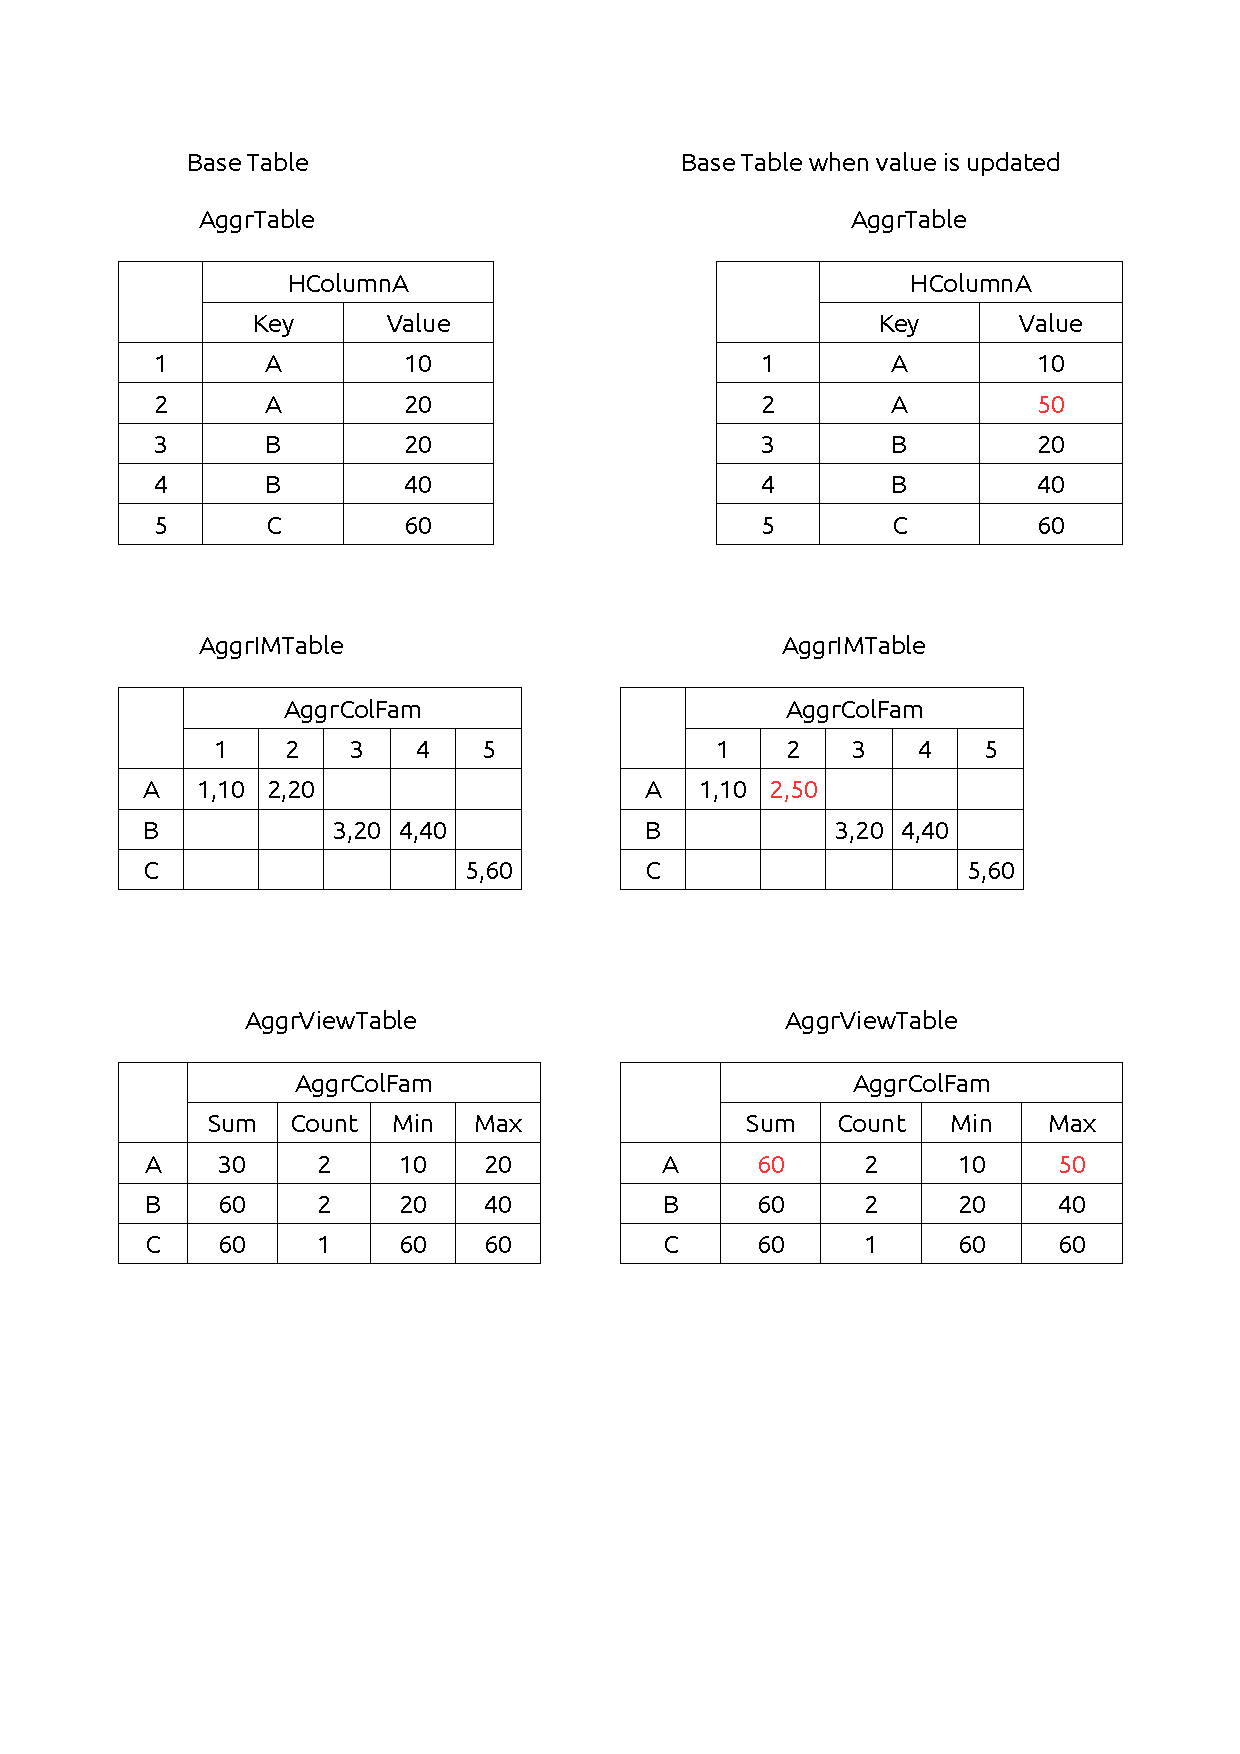
\includegraphics[width=\linewidth]{ValueUpdateAggr}
    \caption{Update value for a existing row key}
    \label{sec:updatevalueforexistingkey}
    
\end{figure}  


\subsubsection{Existing key of a row is updated}
\label{subsubsec:keyupdate}

Whenever there is a trigger to update a Key of the particular rowKey, we first catch the request via prePut() method. In this scenario, we first save key,value pair of the row to be deleted from base table and new key,value pair to be inserted into the base table. Then we release the request and the Key is updated in the base table. In this case, now we have old key,value pair and the new key,value pair. 

In the postPut() method, first we find the column to be deleted from the intermediate table. Then we delete that particular column from the intermediate table. After we delete column from an intermediate table, we need to update aggregation functions in the view table. We create a list and put all the key,value pairs for that particular rowKey of the intermediate table. From the list we update our aggregation functions and then update the result on the view table. After the process is complete without any interruptions, the process is similar as of inserting new key,value pair. We put new key,value pair in our intermediate table and now we need to update aggregation functions in the view table. We create a list and put all the key,value pairs for that particular rowKey of the intermediate table. From the list we update our aggregation functions and then update the result on the view table. In the figure \ref{sec:updateKeyforexistingrow}, the old key $A$ is updated to new key $B$. In the intermediate table, the plotting for old key $A$ is deleted and aggregation functions for old key $A$ are also updated in the view table. After the process is completed, new values for updated key $B$ is plotted in the intermediate table and then the view table for row key $B$ is also updated accordingly.

\begin{figure}
    \centering
    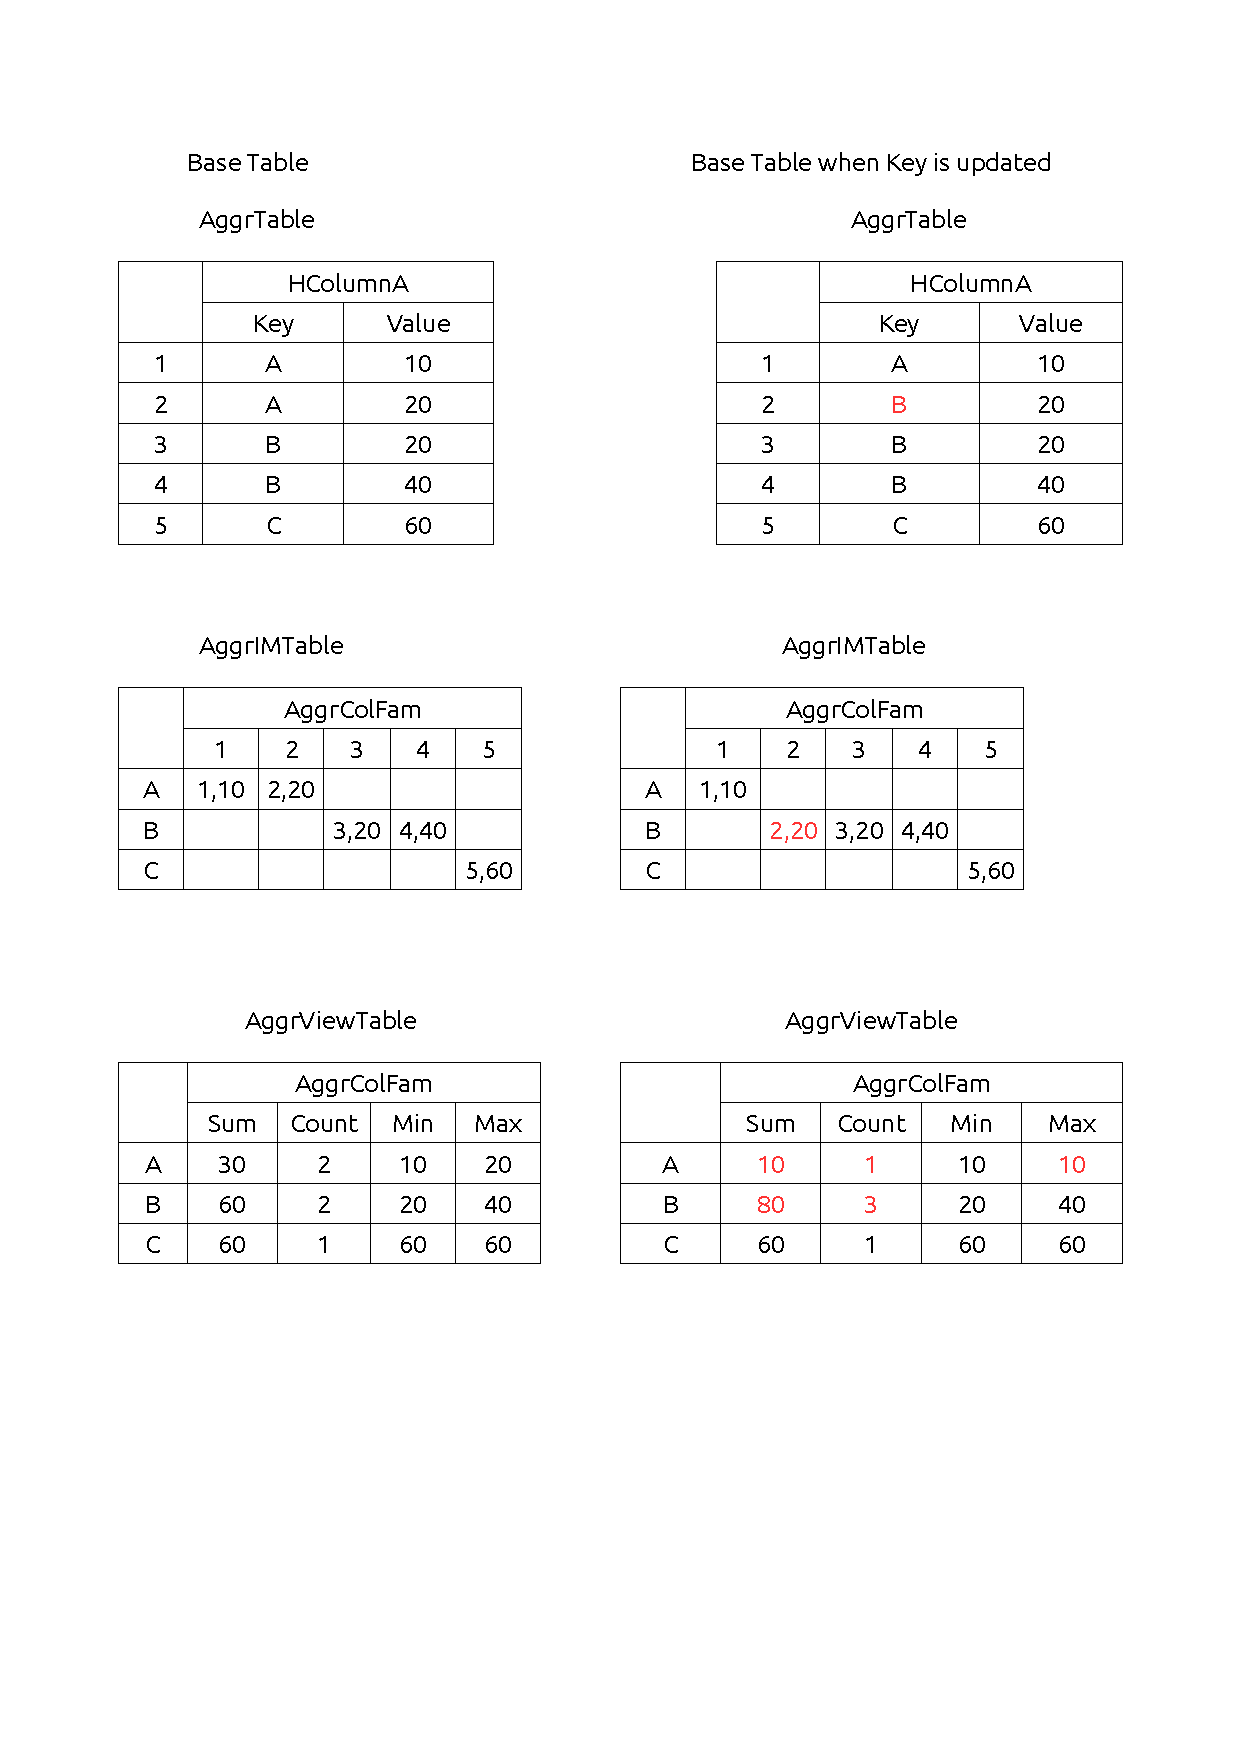
\includegraphics[width=\linewidth]{KeyUpdateAggr}
    \caption{Update Key for a existing row key}
    \label{sec:updateKeyforexistingrow}
    
\end{figure} 

\newpage
\subsubsection{Existing row is deleted}
\label{subsubsec:rowdelete}

When an existing row is deleted in the base table, we first get key,value pair in prePut() method. In the postPut() method of observer coprocessor, we first delete the entry for that particular $key$ from the intermediate table. But before deleting, we have two scenarios here. If the $key$ to be deleted has more than one values in the intermediate table, then we delete the particular plotting in the intermediate table and update aggregation functions for that $key$ in the view table. If the $Key$ in the intermediate table has only one value, then we delete that row from an intermediate table and then also delete the row from view table.

In the figure \ref{sec:deleteexistingrow}, we have a delete() call for row key $5$. The $key$ for row key $5$ is $C$. Now we delete the row key $5$ from the base table. After that, we delete the plotting for key $C$ in our intermediate table. Since the key $C$ has only one plotting, we delete entry for row key $C$ from the view table instead of recomputing aggregation functions for row key $C$. 

\begin{figure}
    \centering
    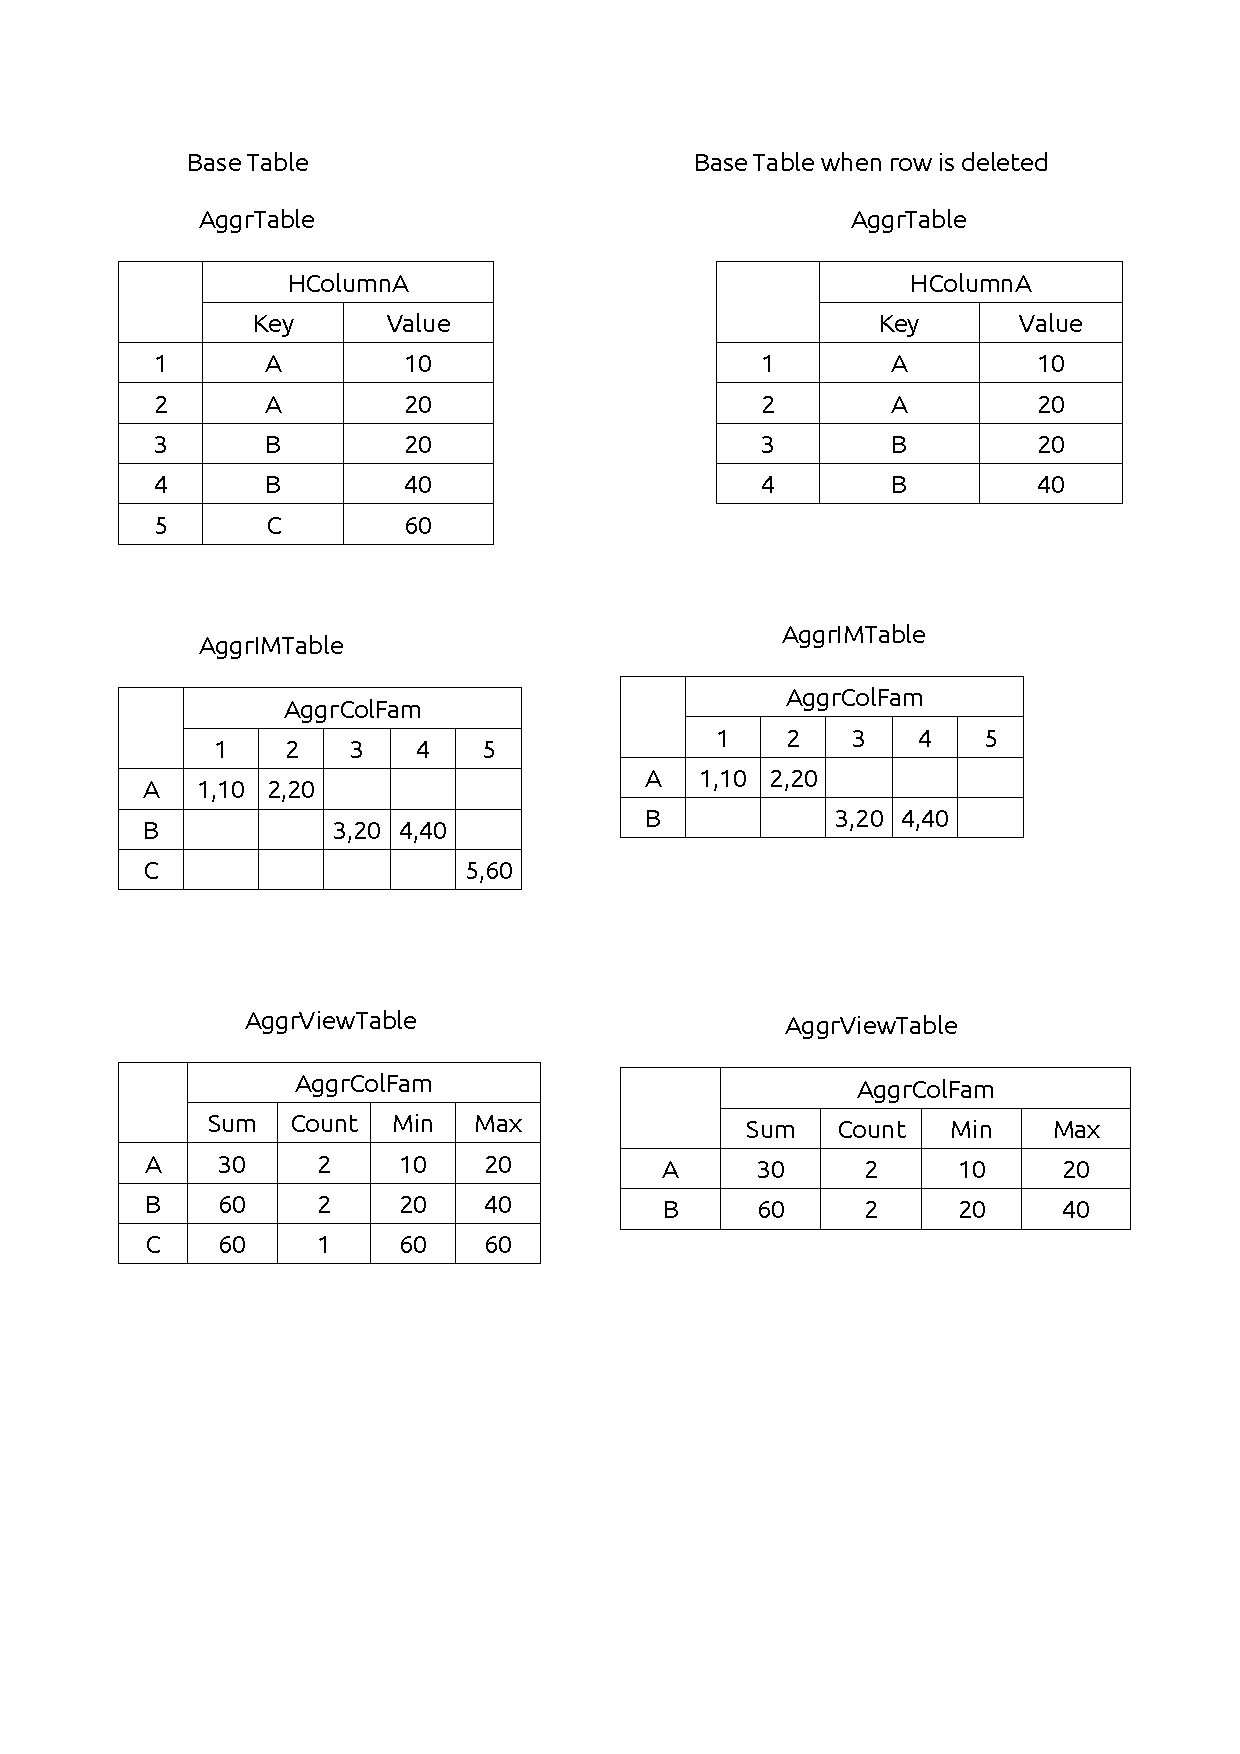
\includegraphics[width=\linewidth]{DeleteExistingRowAggr}
    \caption{Delete an existing row}
    \label{sec:deleteexistingrow}
    
\end{figure} 

\newpage
\subsection{Join and Aggregation}
\label{subsec:joinandaggregation}

For Join and Aggregation, we have two base tables with key,value pairs. We create an intermediate table from two base tables as described in subsection \ref{subsec:intermediatetable}. For Join and Aggregation, we join two base tables on the basis of K-FK join, apply $sum$ aggregation function on the resultset and put result in the view table. In this approach, there are certain scenarios where we have to maintain consistency between base tables and a view table.

%In this subsection, we have implemented Join and Aggregation functionalities. For this, we have joined two base tables and in the view table, we have the sum of the values for a same $key$. We also have an intermediate table where both the base tables are merged by a particular $key$ and values are plotted in the intermediate table base on that $key$. As described in \ref{sec:aggregationImpl}, we have implemented sum for same $key$ in both the base tables. 

%The figure below explains how we map base table to a view table.

%\begin{figure}
%    \centering
%    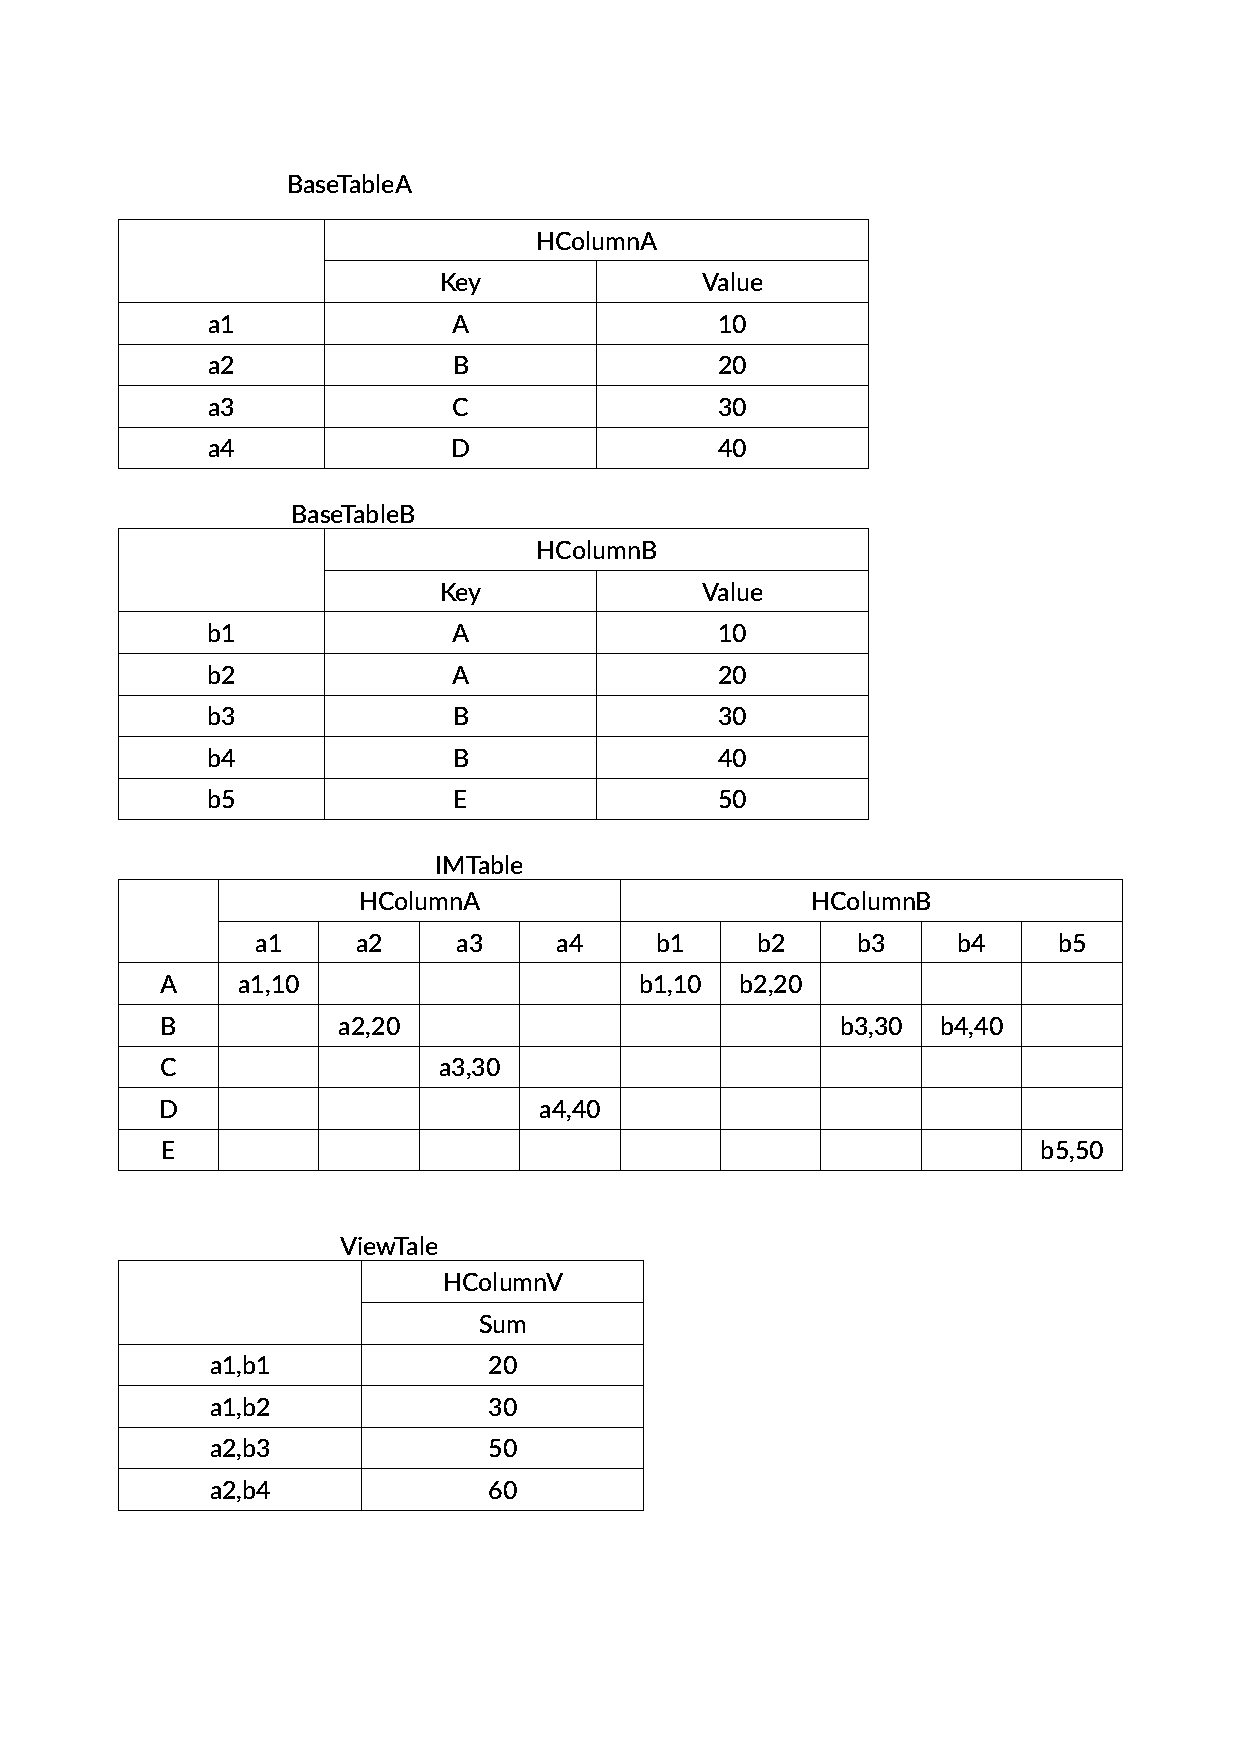
\includegraphics[width=\linewidth]{JoinAndAggregation}
%    \caption{Join and Aggregation}
%    \label{sec:joinandaggregation}
    
%\end{figure}

%\newpage
%There are certain scenarios where coprocessor is triggered for an update and delete operations.

\begin{enumerate}
    \item New row is inserted
    \item Existing value of a row is updated
    \item Existing key of a row is updated
    \item Existing row is deleted
\end{enumerate}

\subsubsection{New row is inserted}

When a client inserts new row with key,value pair in a base table, we have to update our intermediate table and view table accordingly to maintain consistency between them. Updating intermediate table is not a big problem here, we just need to put new key,value pair for that particular rowKey in a corresponding column family. In the prePut() method, we determine the key,value pair to be inserted into the base table. When the request is triggered in postPut() method, we need to update intermediate table and view table accordingly. Since K-FK join is involved, we need to figure out the new rows generated with respect to the newly inserted key,value pair. The first list contains newly inserted key,value pair for that particular rowKey. The second list contains all the key,value pairs for the same rowKey. Now we get a cartesian product of key,value pairs, value containing the sum of the K-FK joins that are to be inserted into the view table. Now the result is inserted into the veiw table. This way, we are able to maintain consistency whenever a new row is inserted in a base table.
The figure \ref{sec:insertnewrowjoinandaggr} describes the scenario in more detail. The updated table on the right has new values plotted in red.

\begin{figure}
    \centering
    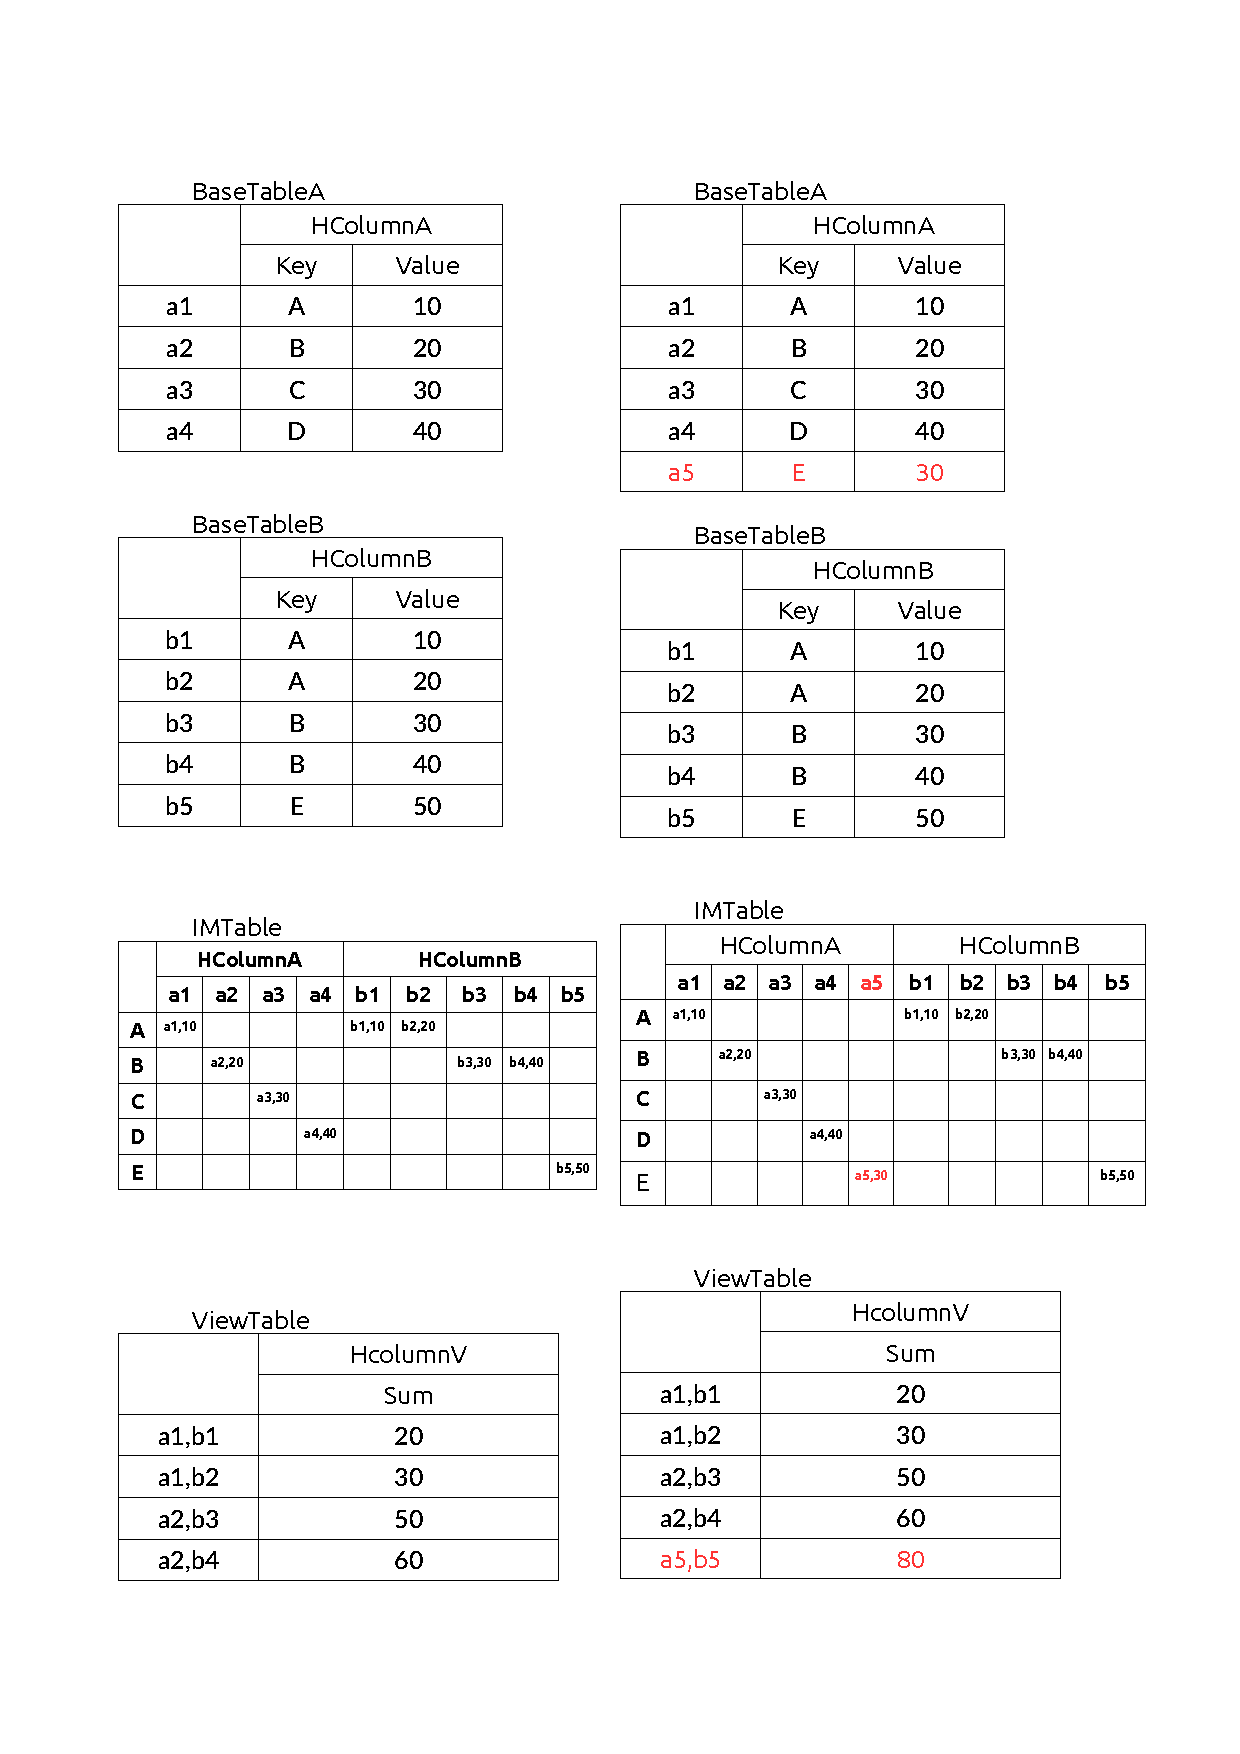
\includegraphics[width=\linewidth]{NewRowInsertJoinAggr}
    \caption{New row is inserted for Join and Aggregation}
    \label{sec:insertnewrowjoinandaggr}
    
\end{figure}

\newpage

\subsubsection{Existing value of a row is updated}
%When a value of a $key$ is updated in the base table, the consistency should also be maintained in the view table. So when the base table is updated, the request is triggered by the postPut() method and intermediate table and view tables are updated accordingly.

When an existing value of a particular key is updated in a base table, we update the particular value in our intermediate table. In the prePut() method, we determine key,value pair for the row to be updated and in the postPut() method, we update our intermediate table and view table accordingly. The update process in an intermediate table is straightforward i.e. we just update value for that particular row and column. Now in order to update our view table, we need to find all the rows that are affected by an update statement as K-FK join is involved. We create two lists and the first list contains key,value pair of the row which was just updated. The second list contains all the key,value pairs for the same rowKey. Now we get a cartesian product of key,value pairs, and the value containing sum of K-FK joins that are to be updated into the view table. This way we maintain consistency between base tables and view table when an existing row is updated in the base table.

\subsubsection{Existing key of a row is updated}
%As described in \ref{subsubsec:keyupdate}, when $key$ is modified in the base table, we first have to delete an entry from the intermediate table and view table if the row exists for that particular $key$. Once delete operation is completed without interruption, then we insert the updated key in the intermediate table and view table.

In this scenario, we first save key,value pair of the row to be deleted from base table in prePut() method. After the entry has been deleted from the base table, we delete an entry from the intermediate table in the postPut() method. Now we have to find all the rows to be deleted from the view table for that particular key. In this process, we create two list and find out all the rows to be deleted from the view table. The first list contains key,value pair which we saved earlier. The second list contains all the key,value pairs for the same rowKey. Now we get a cartesian product of key,value pairs that are to be deleted from the view table. Then we delete all the affected rows from the view table. Now we have to update old key to a new key in a base table. Once the base table has been updated, we update our intermediate table accordingly. Now we need to find out the rows to be inserted into the view table as it involves K-FK join among the base tables. We do that by creating two lists, first list containing new key,value pair and second list containing all the key,value pairs for that rowKey. Now we get a cartesian product of key,value pairs, and the value containing sum of K-FK joins that are to be inserted into the view table.

\subsubsection{Existing row is deleted}
%The implementation for this scenario is same as described in subsection \ref{subsubsec:rowdelete}. The entry is first deleted from the base table, and if an entry exists in the intermediate table and view table, the entries are deleted from those table accordingly.

When a row is deleted from the base table, we simply delete an entry from the intermediate table. The next task is to find all the rows that are to be deleted from the view table. This is a similar process as described in the sub section above. We first create two lists here, first list contains the key,value pair of the row that was deleted and the second row contains all the key,value pairs for the same row. Now we get a cartesian product of key,value pairs that are to be deleted the view table. We delete all the rows from the view table. This way we can maintain consistency between base table and view table when a row is deleted from the base table.

\subsection{Join and Selection}
\label{subsec:joinandselection}

The approach implemented in this subsection is similar to the approach described in subsection \ref{subsec:joinandaggregation}. We have two base tables with key,value pairs. We create an intermediate table from two base tables as described in subsection \ref{subsec:intermediatetable}. For Join and Selection, we join two base tables on the basis of K-FK join and put result in the view table. In this approach, there are also certain scenarios where we have to maintain consistency between base tables and a view table.

\begin{enumerate}
	\item New row is inserted
	\item Existing value of a row is updated
	\item Existing key of a row is updated
	\item Existing row is deleted
\end{enumerate}

\subsubsection{New row is inserted}
\label{New row is inserted JoinSelection}
When a client inserts new row with key,value pair in a base table, we have to update our intermediate table and view table accordingly to maintain consistency between them. Updating intermediate table is not a big problem here, we just put new key,value pair for that particular rowKey in a corresponding column family. Since K-FK join is involved, we need to figure out the new rows generated with respect to the newly inserted key,value pair. The first list contains newly inserted key,value pair for that particular rowKey. The second list contains all the key,value pairs for the same rowKey. Now we get a cartesian product of key,value pairs that are to be inserted into the view table. Now we are able to maintain consistency whenever a new row is inserted in a base table.

\subsubsection{Existing value of a row is updated} 
When an existing value of a particular key is updated in a base table, we update the particular value in our intermediate table. The update process in an intermediate table is straightforward i.e. we just update value for that particular row and column. Now in order to update our view table, we need to find all the rows that are affected by an update statement. We create two lists and the first list contains key,value pair of the row which was just updated. The second list contains all the key,value pairs for the same rowKey. Now we get a cartesian product of key,value pairs that are to be updated into the view table. This way we maintain consistency between base tables and view table when an existing row is updated in the base table.


\subsubsection{Existing key of a row is updated}
In this scenario, we first save key,value pair of the row to be deleted from base table. After the entry has been deleted from the base table, we delete an entry from the intermediate table. Now we have to find all the rows to be deleted from the view table for that particular key. In this process, we create two list and find out all the rows to be deleted from the view table. The first list contains key,value pair which we saved earlier. The second list contains all the key,value pairs for the same rowKey. Now we get a cartesian product of key,value pairs that are to be deleted from the view table. Then we delete all the affected rows from the view table. Now we have to update old key to a new key in a base table. Once the base table has been updated, we update our intermediate table accordingly. Now we need to find out the rows to be inserted into the view table as it involves K-FK join among the base tables. We do that by creating two lists, first list containing new key,value pair and second list containing all the key,value pairs for that rowKey. Now we get a cartesian product of key,value pairs that are to be inserted into the view table.

\subsubsection{Existing row is deleted}
When a row is deleted from the base table, we simply delete an entry from the intermediate table. The next task is to find all the rows that are to be deleted from the view table. This is a similar process as described in the sub section above. We first create two lists here, first list contains the key,value pair of the row that was deleted and the second row contains all the key,value pairs for the same row. Now we get a cartesian product of key,value pairs that are to be deleted the view table. We delete all the rows from the view table. This way we can maintain consistency between base table and view table when a row is deleted from the base table.

\newpage
\chapter{Evaluation}
\label{Evaluation}
In this chapter we perform different kinds of experiments on both Pseudo Distributed mode (single node cluster) and Fully Distributed mode (multi node cluster). We will further discuss about every types of experiments we performed and the dataset we used. We will then present the result of our experiments.

\section{Experiment Setup (Pseudo Distributed Mode)}
In pseudo distributed mode, we have performed four different kinds of experiments for each of the three scenarios. First experiment $View$ $Re$-$computation$ $vs$ $Maintenance$ is performed on three different datasets while rest of the experiments are performed on fixed dataset.

\subsection{Deployment}
We performed our experiment on a single node cluster (Ubuntu 16.04 LTS, Intel Core i5-3230M CPU @ 2.60GHz, 3.9GB RAM, 23GB HD). We installed hadoop in pseudo distributed mode. The services like JobTracker, TaskTracker, Namenode and Datanode runs as a separate Java process in a single cluster. We installed hadoop version 2.6.4 and hbase version 1.1.5 for our experiments.

\subsection{Table Configuration}
\label{Table Configuration standalone}
For $Aggregation$, we first create one empty base table, an intermediate table and a view table. We first insert records in the base table. After that, we read data from base table and write into intermediate table as explained in section \ref{sec:aggregationImpl}. Once write in the intermediate table is completed, we perform different aggregation functions like $Sum$, $Max$, $Min$ and $Count$ based on the $key$ of intermediate table and write the result in view table.
\linebreak
\linebreak
For $Join$ \& $Aggregation$ and $Join$ \& $Selection$, we create two base tables as it involves k-kf joins, an intermediate table and a view table. We first insert records in both the base tables, read data from first base table and insert into first column family of an Intermediate table, and again read data from second base table and insert into second column family of an Intermediate table as explained in sections \ref{subsec:joinandaggregation} and \ref{subsec:joinandselection} respectively. After we have our Intermediate table ready, we apply k-kf join and insert data into view table accordingly.

\subsection{Control Parameter}
\label{Control Parameter}
There are certain control parameters defined for our experiments to determine performance.

\begin{description}
	\item[$\bullet$]  $noOfRegions$: The number of regions within a Region Server 
\end{description}

\begin{description}
	\item[$\bullet$]  $typesOfOperation$: The type of operation performed by the client. In our experiment, we've performed insert, update and delete operation. 
\end{description}

\begin{description}
	\item[$\bullet$]  $typesOfViews$: This parameter defines the types of views we have implemented in our experiments such as $Join$, $Selection$, $Sum$, $Count$, $Max$, $Min$. 
\end{description}

\begin{description}
	\item[$\bullet$]  $timeInMillis$: This parameter defines the time taken in milliseconds to perform certain operations. 
\end{description}

\section{Experiment 1 (Aggregation)}
\label{(sec:AggrExp)}
To evaluate the performance of $Aggregation$ view type, we perform three different experiments. In the first experiment, we compare the single region execution time for $View\Re$-$computation$ and $Incremental \  maintenance$ on three different datasets. Next, we perform the same experiments on a dataset with 100,000 records by varying the number of regions on a single region server.
 
\subsection{Aggregation: View Re-computation vs Maintenance}
% In the first set, we insert 10.000 rows in the base table and we compute intermediate table and view tables accordingly. In the view table, we compute four different aggregation functions $Sum$, $Count$, $Min$ and $Max$. When client issues any update operation, either we re-compute view table from scratch and compute aggregation functions or we update view table incrementally. The graph shows time taken to re-compute view table vs time taken to update view table incrementally for each type of update operations. We conduct same experiment for 1.00.000 and 2.50.000 records. From the graph, we see that updating view table incrementally saves significant amount of time than re-computing view table for every client operation. The graph below shows time required in millisecond to recompute view table and incrementally update view table.

To evaluate performance in View Re-computation vs Maintenance, we first create a base table with 10,000 rows and generate corresponding intermediate and view tables. The view table consists of four different aggregations of the base table data, namely $Sum$, $Count$, $Min$ and $Max$. For operation in a base table, view table can be updated to reflect changes in two different ways, (a) re-compute (b) incremental update. In our experiments, we compare the execution time for these two methods. Further, we perform the experiments for 100,000 and 250,000 records. In our experiments, we report the execution time in milliseconds. In the figure \ref{sec:AggrExpStandalone}, in x-axis, we show types of client operations performed in base table and in y-axis we show performance optimized in percent. 

\begin{figure}
	\centering
	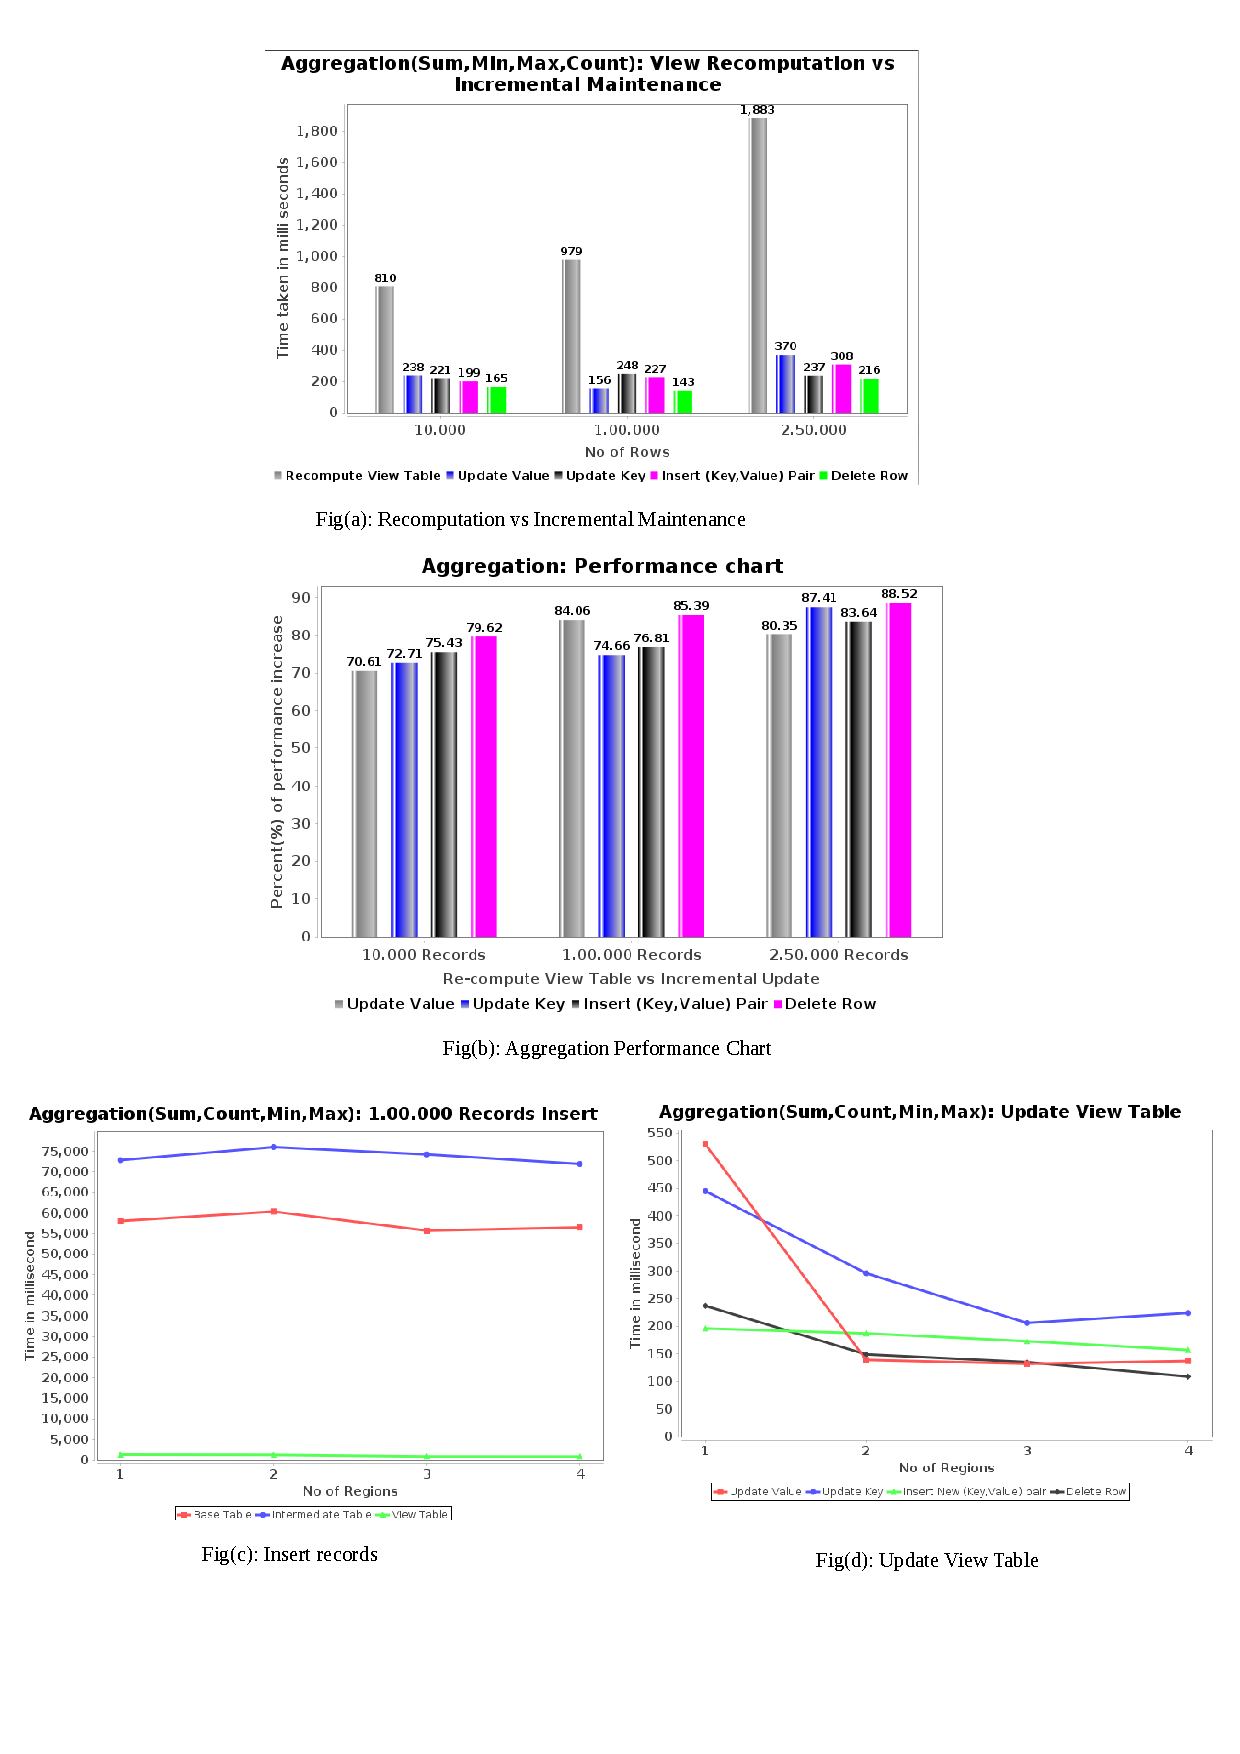
\includegraphics[width=\linewidth]{Aggregation_exp1_standalone}
	\caption{Aggregation Experiment Standalone}
	\label{sec:AggrExpStandalone}
\end{figure} 
\newpage
% In the figure \ref{sec:AggrExpStandalone}, $Fig(a)$ shows the time taken to insert records in view table vs update view table incrementally whenever there is an update in the base table. This experiment is run in three different datasets and in each datasets we know that updating view table takes significantly less amount of time than recomputing view table. Fig(d) shows shows the performance calculated in recomputing base table vs incremental maintenance. In the x-axis, we show types of client operations performed in base table and in y-axis we show performance optimized in percent. We calculate performance using the formula,
In Figure \ref{sec:AggrExpStandalone}, $Fig(a)$, we compare the time taken while inserting records using the above methods. In figure \ref{sec:AggrExpStandalone}, $Fig(a)$, we observe that incremental update outperforms re-compute method by orders of magnitude. Further, In Fig \ref{sec:AggrExpStandalone}, $Fig(b)$, we report the percentage improvement achieved by an incremental update for four different operations over the re-compute baseline. Here we observe that incremental method yields up to 88\% improvement over the baseline.
\newline
\begin{align*}
\text{performance} = \frac{\text{time taken to compute view table} - \text{incremental update}}{\text{time taken to compute view table}} \times 100
\end{align*}
	 
% One of the reasons for this performance optimization is that when recomputing a view table, we first have to perform read operation on base table and then write operation on view table. In incremental maintenance approach, only write operation is performed for every rows affected by the client operation on base table. The other reason is that the no. of rows updated in view table are less in comparison to the total no of rows in the base table. %
The reason for the significant improvement in performance of incremental update over the baseline is due to read-write and recompute overhead.
In the re-compute method, we need to read the whole base table and
reconstruct the view table. However, in the incremental method, we do not reconstruct the view table but only update the rows that are affected by the operation on the base table. 

\subsection{Aggregation: Insert Records}
\label{Insert Records Aggr}

In this experiment, we wanted to prove that splitting table across multiple regions improves overall performance. In the figure \ref{sec:AggrExpStandalone}, $Fig(c)$, in x-axis we show no. of regions and in y-axis, we show time taken to insert records in millisecond. To prove our hypothesis, we first inserted 1.00.000 records without splitting a table and recorded time taken to insert records. In the second scenario, we split our table in two regions and note time taken to insert 1.00.000 records. We carried out same experiment by splitting our table in three and four regions simultaneously. We noted time taken for each experiments and plotted a graph. From the graph, we see that splitting our table across regions takes less time to insert 1.00.000 records. The reason for this improvement is that the table is split horizontally across all the regions. The $HexStringSplit$ algorithm partitions the table evenly across all the regions, as a result of which the load is distributed equally among all the regions.


%We ran this experiment to see how it affects the result if we split our tables in multiple regions. We wanted to show that we can improve performance if we split our tables in multiple regions within a region server. In the figure \ref{sec:AggrExpStandalone}, $Fig(b)$ shows that if we split our table in multiple regions, we can reduce the insert operation in our tables. In x-axis we show no. of regions and in y-axis we show time taken in milliseconds to insert records in base table, intermediate table and view table. From the graph we see that, the more no. of regions the less time it takes to insert records. %

\subsection{Aggregation: Update View Table} 
\label{Update View Table Aggr}
In section \ref{Insert Records Aggr}, we proved that we can improve optimization if we split our tables across multiple regions. In this experiment, we wanted to see how it affects the performance if we split $View$ $Table$ across multiple regions. In the figure \ref{sec:AggrExpStandalone}, $Fig(c)$, in x-axis we show no. of regions and in y-axis, we show time taken to update view table incrementally in millisecond. We first insert 1.00.000 records in base table and pre-compute view tables accordingly. In the first scenario, we compute view table without pre-splitting view table. In the second scenario, we pre-split view table across two regions. Similarly, we also pre-split view table across three and four regions and compute view tables accordingly. When client issues update operation on base table, we reflect changes in view table incrementally and note time taken for each type of update operation. Then we plot graph with the captured results and from $Fig(d)$, we proved that splitting table across multiple regions can improve overall performance. 

\section{Experiment 2 (Join and Aggregation)}
\label{(sec:Join and Aggregation Exp)} 
For $Join$ \& $Aggregation$, we create two base tables as it involves K-FK joins, an intermediate table and a view table. We insert 3.000 rows in both the base table, apply K-FK joins and calculate sum for those joins and insert result in the view table. We then run experiments to see how we can improve performance as we split our tables across multiple regions.

\subsection{Join and Aggregation: Insert records}
\label{Join and Aggregation: Insert records Standalone}
In this experiment, we insert 3.000 records in each of the base tables and apply K-FK join in the two base tables. First we run this experiment in a single region and see the number of rows generated in the view table after applying K-FK joins. We run this experiment for 2, 3 and 4 regions and split our tables accordingly. In the figure \ref{sec:JoinAggrExpStandalone}, Fig(a) shows the graph of no. of records inserted in view tables. We use this statistics for running other sub-experiments.

\subsection{Join and Aggregation: View Re-computation vs Maintenance}
\label{Join and Aggregation: View Re-computation vs Maintenance Standalone}
In this experiment, we wanted to show that by incrementally maintaining our view tables, we can increase the overall performance of the system. We ran this experiment on the basis of data gathered in sub-section \ref{Join and Aggregation: Insert records Standalone}. As a proof, we first ran this experiment on dataset of 1.53.761 records. From the graph \ref{sec:JoinAggrExpStandalone}, $Fig(b)$ shows the time required for re-computing view table vs time required to incrementally update view table. If we need to re-compute view table, in such scenario, we first need to perform read operation on the entire base table and then write operation in view table. Whereas in incremental maintenance, we only update the affected rows in view table. To ensure our hypothesis works, we ran our experiment on bigger dataset of 3.45.658 rows. From the experiment results, we proved that maintaining views incrementally is significantly less expensive than re-computing view table for every client request in base table.

\subsection{Join and Aggregation: Insert Records}
\label{Join and Aggregation: Insert Records Standalone}
We ran this experiment on the basis of data collected in section \ref{Join and Aggregation: Insert records Standalone}. In this experiment, we split our tables into multiple regions, and we want to show that splitting table across multiple regions enhances performance of the system. From the graph \ref{sec:JoinAggrExpStandalone}, $Fig(c)$ shows that we were able to optimize performance by splitting tables into multiple regions. In x-axis we show no. of regions and in y-axis we show time taken in milliseconds to insert records in base table, intermediate table and view table.

\subsection{Join and Aggregation: Update View Table} 
\label{Join and Aggr: Update View Table Standalone}
In section \ref{Join and Aggregation: Insert Records Standalone}, we showed that client operation time can be reduced significantly if we split our tables across multiple regions. In this section,we ran an experiment to see how we are able to optimize performance if we split $View$ $Table$ across multiple regions. For that, we split $View$ $Table$ across multiple regions and ran this experiment. From the graph \ref{sec:JoinAggrExpStandalone}, $Fig(d)$ proved that we also can reduce operation time if we split $View$ $Table$ across multiple regions. In x-axis we show no. of regions and in y-axis we show time in milliseconds required to complete client operation. We ran this experiment on different types of client operations and for each operation we were able to decrease time taken to complete required operation. 

\begin{figure}
	\centering
	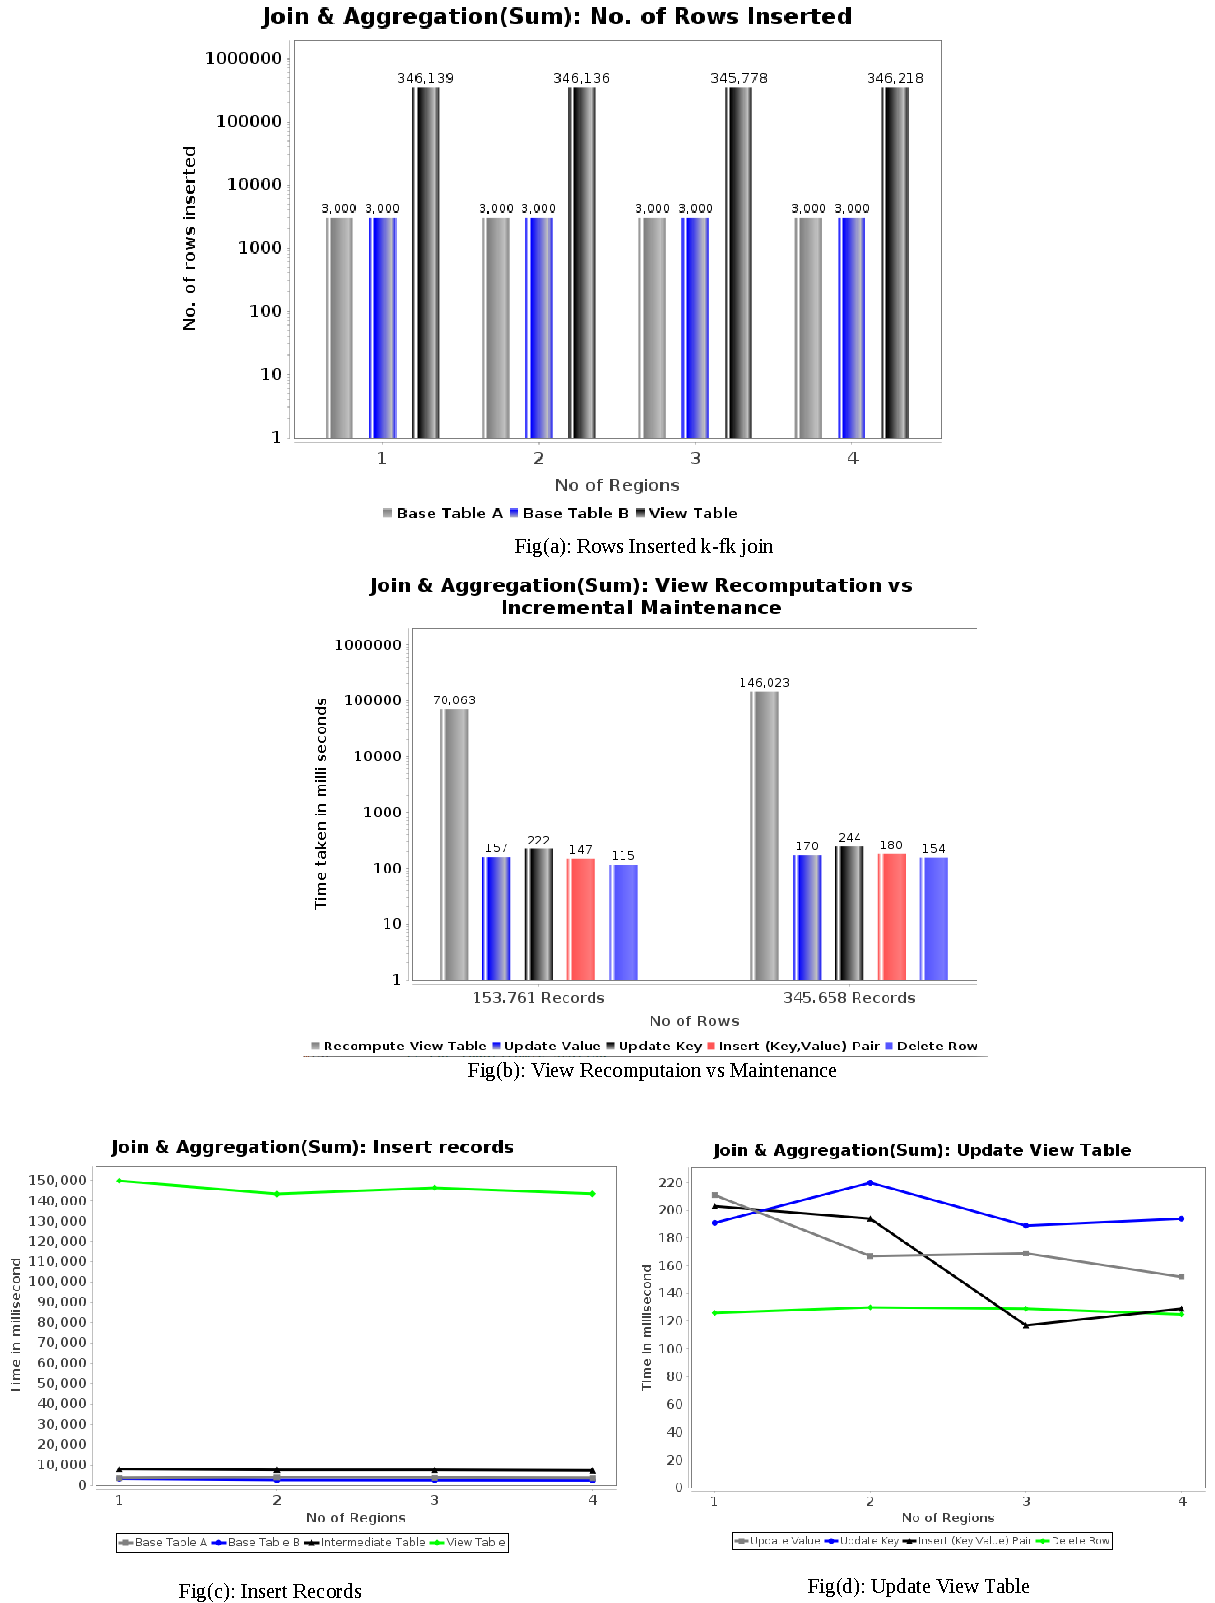
\includegraphics[width=\linewidth]{JoinAndAggr_exp_standalone}
	\caption{Join and Aggregation Experiment Standalone}
	\label{sec:JoinAggrExpStandalone}
	
\end{figure} 
\newpage

\section{Experiment 3 (Join and Selection)}
\label{(sec:Join and Selection Exp Standalone)} 
For $Join$ \& $Selection$, we create two base tables as it also involves K-FK joins, an intermediate table and a view table. We insert 3.000 rows in both the base table, apply K-FK joins and select values for those joins and insert result in the view table. We then run experiments to see how we can improve performance as we split our tables across multiple regions.

\subsection{Join and Selection: Insert records}
\label{Join and Selection: Insert records Standalone}
In this experiment, we insert 3.000 records in each of the base tables and apply K-FK join in the two base tables. First we run this experiment in a single region and see the number of rows generated in the view table after applying K-FK joins. We run this experiment for 2, 3 and 4 regions and split our tables accordingly across those regions. In the figure \ref{sec:JoinSelExpStandalone}, Fig(a) shows the graph of no. of records inserted in view tables. We use this statistics for running other sub-experiments.

\subsection{Join and Selection: View Re-computation vs Maintenance}
\label{Join and Selection: View Re-computation vs Maintenance Standalone}
In this experiment, we wanted to show that by incrementally maintaining our view tables, we can increase the overall performance of the system. We ran this experiment on the basis of data gathered in sub-section \ref{Join and Selection: Insert records Standalone}. As a proof, we first ran this experiment on dataset of 1.53.561 records. From the graph \ref{sec:JoinSelExpStandalone}, $Fig(b)$ shows the time required for re-computing view table vs time required to incrementally update view table. If we need to re-compute view table, in such scenario, we first need to perform read operation on the entire base table and then write operation in view table. Whereas in incremental maintenance, we only update the affected rows in view table. To ensure our hypothesis works, we ran our experiment on bigger dataset of 3.45.049 rows. From the experiment results, we proved that maintaining views incrementally is significantly less expensive than re-computing view table for every client request in base table.

\subsection{Join and Selection: Insert Records}
\label{Join and Selection: Insert Records Standalone}
We ran this experiment on the basis of data collected in section \ref{Join and Selection: Insert records Standalone}. In this experiment, we split our tables into multiple regions, and we want to show that splitting table across multiple regions enhances performance of the system. From the graph \ref{sec:JoinSelExpStandalone}, $Fig(c)$ shows that we were able to optimize performance by splitting tables into multiple regions. In x-axis we show no. of regions and in y-axis we show time taken in milliseconds to insert records in base table, intermediate table and view table.

\subsection{Join and Selection: Update View Table} 
\label{Join and Sel: Update View Table Standalone}
In section \ref{Join and Selection: Insert Records Standalone}, we showed that client operation time can be reduced significantly if we split our tables across multiple regions. In this section,we ran an experiment to see how we are able to optimize performance if we split $View$ $Table$ across multiple regions. For that, we split $View$ $Table$ across multiple regions and ran this experiment. From the graph \ref{sec:JoinSelExpStandalone}, $Fig(d)$ proved that we also can reduce operation time if we split $View$ $Table$ across multiple regions. In x-axis we show no. of regions and in y-axis we show time in milliseconds required to complete client operation. We ran this experiment on different types of client operations and for each operation we were able to decrease time taken to complete required operation. 

\section{Experiment Setup (Fully Distributed Mode)}
In fully distributed mode, we have performed four different kinds of experiments for each of the three scenarios. First experiment $View$ $Re$-$computation$ $vs$ $Maintenance$ is performed on three different datasets while rest of the two experiments are performed on fixed dataset.

\subsection{Deployment}
We performed our experiment on a multi node cluster of 3 nodes, two of them are slave nodes and one is master node. We installed two virtual machines for the slave nodes and the master node running as a primary operating system. The master node is running on a computer server (Ubuntu 16.04 LTS, Intel Core i5-3230M CPU @ 2.60GHz x 4, 7.7GB RAM, 364.5GB HD). Both the slave nodes were running on a computer server (Ubuntu 16.04 LTS, Intel Core i5-3230M CPU @ 2.60GHz, 2.0GB RAM, 30.3GB HD). We installed hadoop in fully distributed mode. The services like JobTracker, TaskTracker, Namenode and Datanode runs as a separate Java process in a multiple cluster. We installed hadoop version 2.6.4 and hbase version 1.1.5 for our experiments. DataNode, TaskTracker runs on the slave machine whereas Namenode and JobTracker runs on the master. We have three Region servers, each running on master and slaves respectively.

\subsection{Table Configuration}
The table configuration for fully distributed is similar to pseudo distributed mode as described in sub-section \ref{Table Configuration standalone}.

\begin{figure}
	\centering
	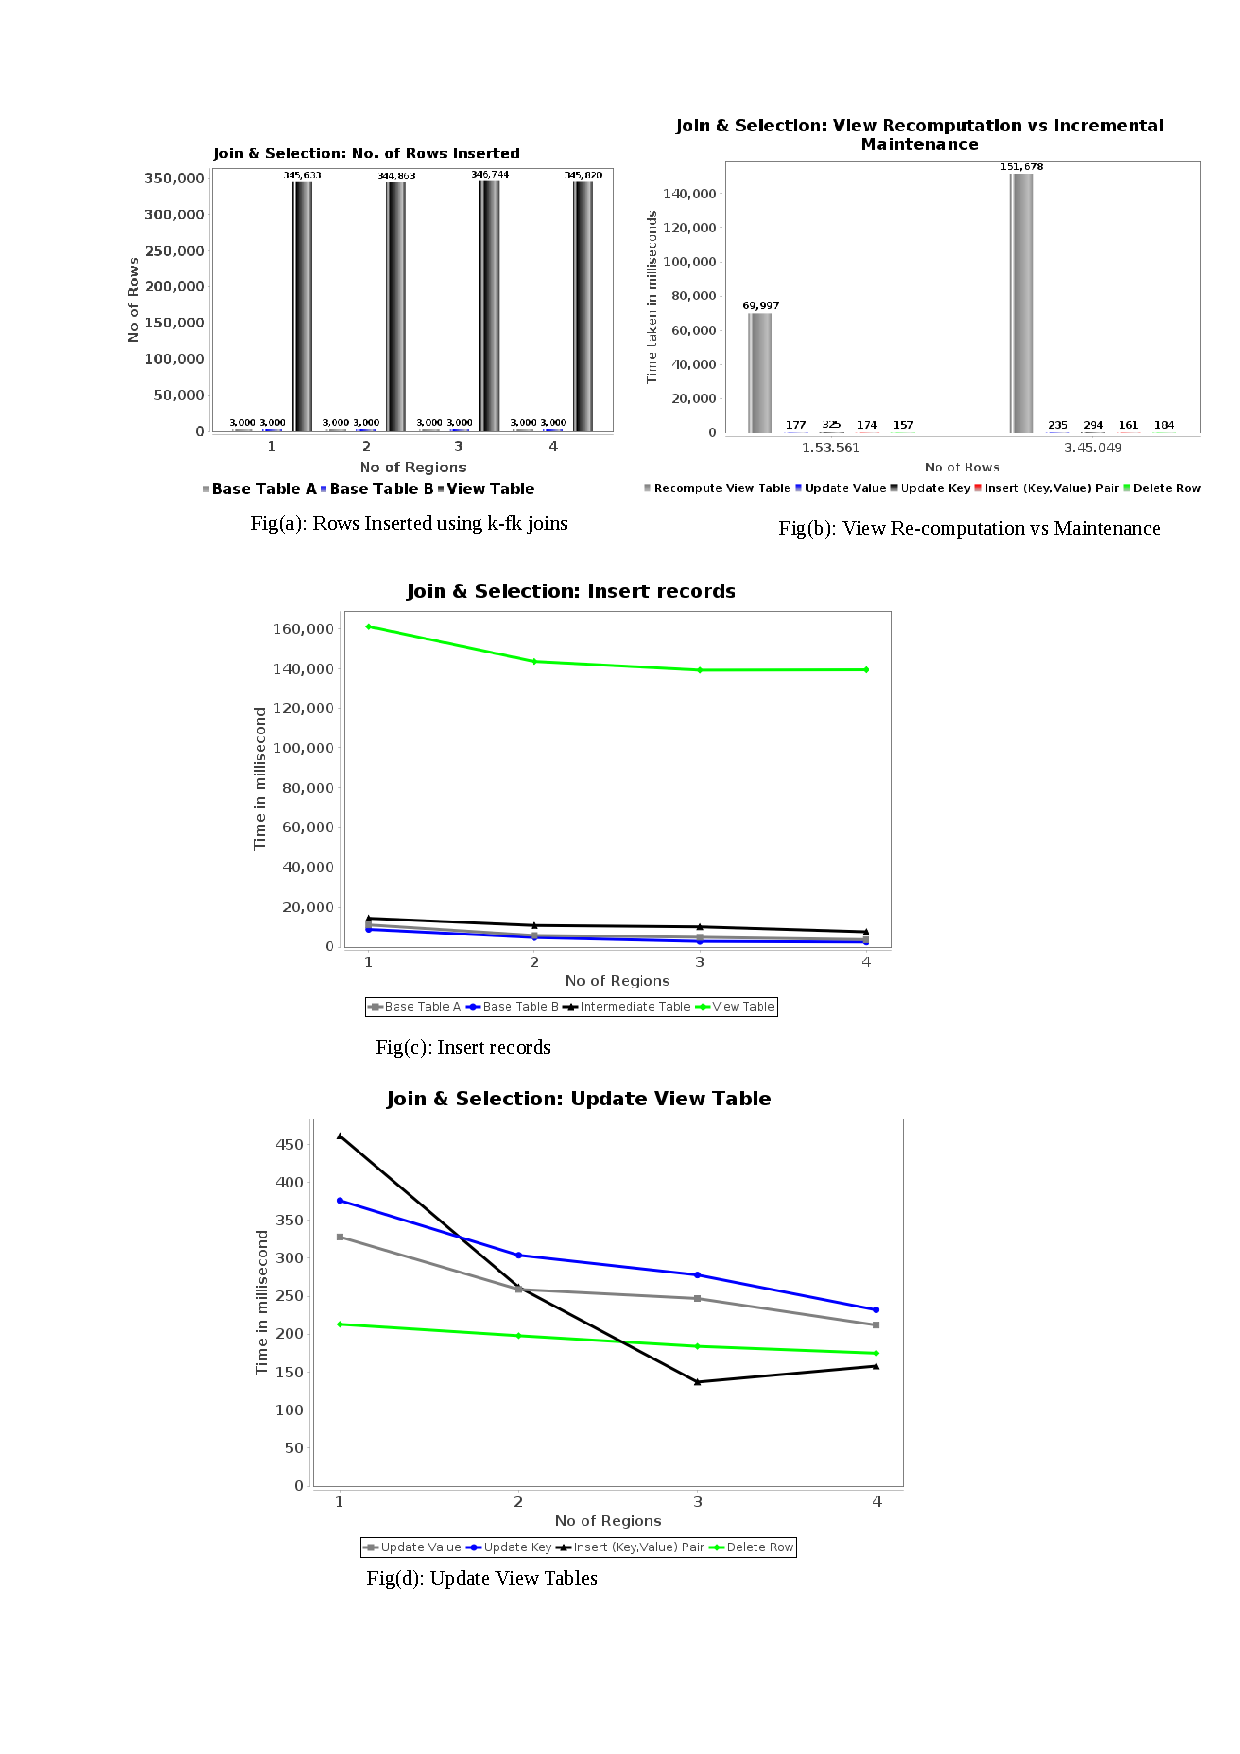
\includegraphics[width=\linewidth]{JoinAndSel_exp_standalone}
	\caption{Join and Selection Experiment Standalone}
	\label{sec:JoinSelExpStandalone}
	
\end{figure} 
\newpage

\subsection{Control Parameter}
\label{Control Parameter Distributed}
There are certain control parameters defined for our experiments to determine performance.

\begin{description}
	\item[$\bullet$]  $noOfRegionServers$: The number of Region Servers. Each Region Server can have one or many regions
\end{description}

\begin{description}
	\item[$\bullet$]  $noOfRegions$: The number of regions within a Region Server 
\end{description}

\begin{description}
	\item[$\bullet$]  $typesOfOperation$: The type of operation performed by the client. In our experiment, we've performed insert, update and delete operation. 
\end{description}

\begin{description}
	\item[$\bullet$]  $typesOfViews$: This parameter defines the types of views we have implemented in our experiments such as $Join$, $Selection$, $Sum$, $Count$, $Max$, $Min$. 
\end{description}

\begin{description}
	\item[$\bullet$]  $timeInMillis$: This parameter defines the time taken in milliseconds to perform certain operations. 
\end{description}

\section{Experiment 4 (Aggregation)}
\label{(sec:AggrExpDist)}
In this experiment, we perform three different sub set of experiments to see how we can improve performance by incrementally maintaining consistency between base table and view table. In this experiment, we have three region servers, two region servers running on slave machines and one region server running on master. 

\subsection{Aggregation: View Re-computation vs Maintenance}
To evaluate performance in View Re-computation vs Maintenance, we first create a base table with 1.00.000 rows and generate corresponding intermediate and view tables. The view table consists of four different aggregations of the base table data, namely $Sum$, $Count$, $Min$ and $Max$. For operation in a base table, view table can be updated to reflect changes in two different ways, (a) re-compute (b) incremental update. In our experiments, we compare the execution time for these two methods. Further, we perform the experiments after splitting table across multiple regions. In our experiments, we report the execution time in milliseconds. In the figure \ref{sec:AggrExpDist}, in x-axis, we show no. of regions and in y-axis we show time taken to insert records in millisecond. 


\begin{figure}
	\centering
	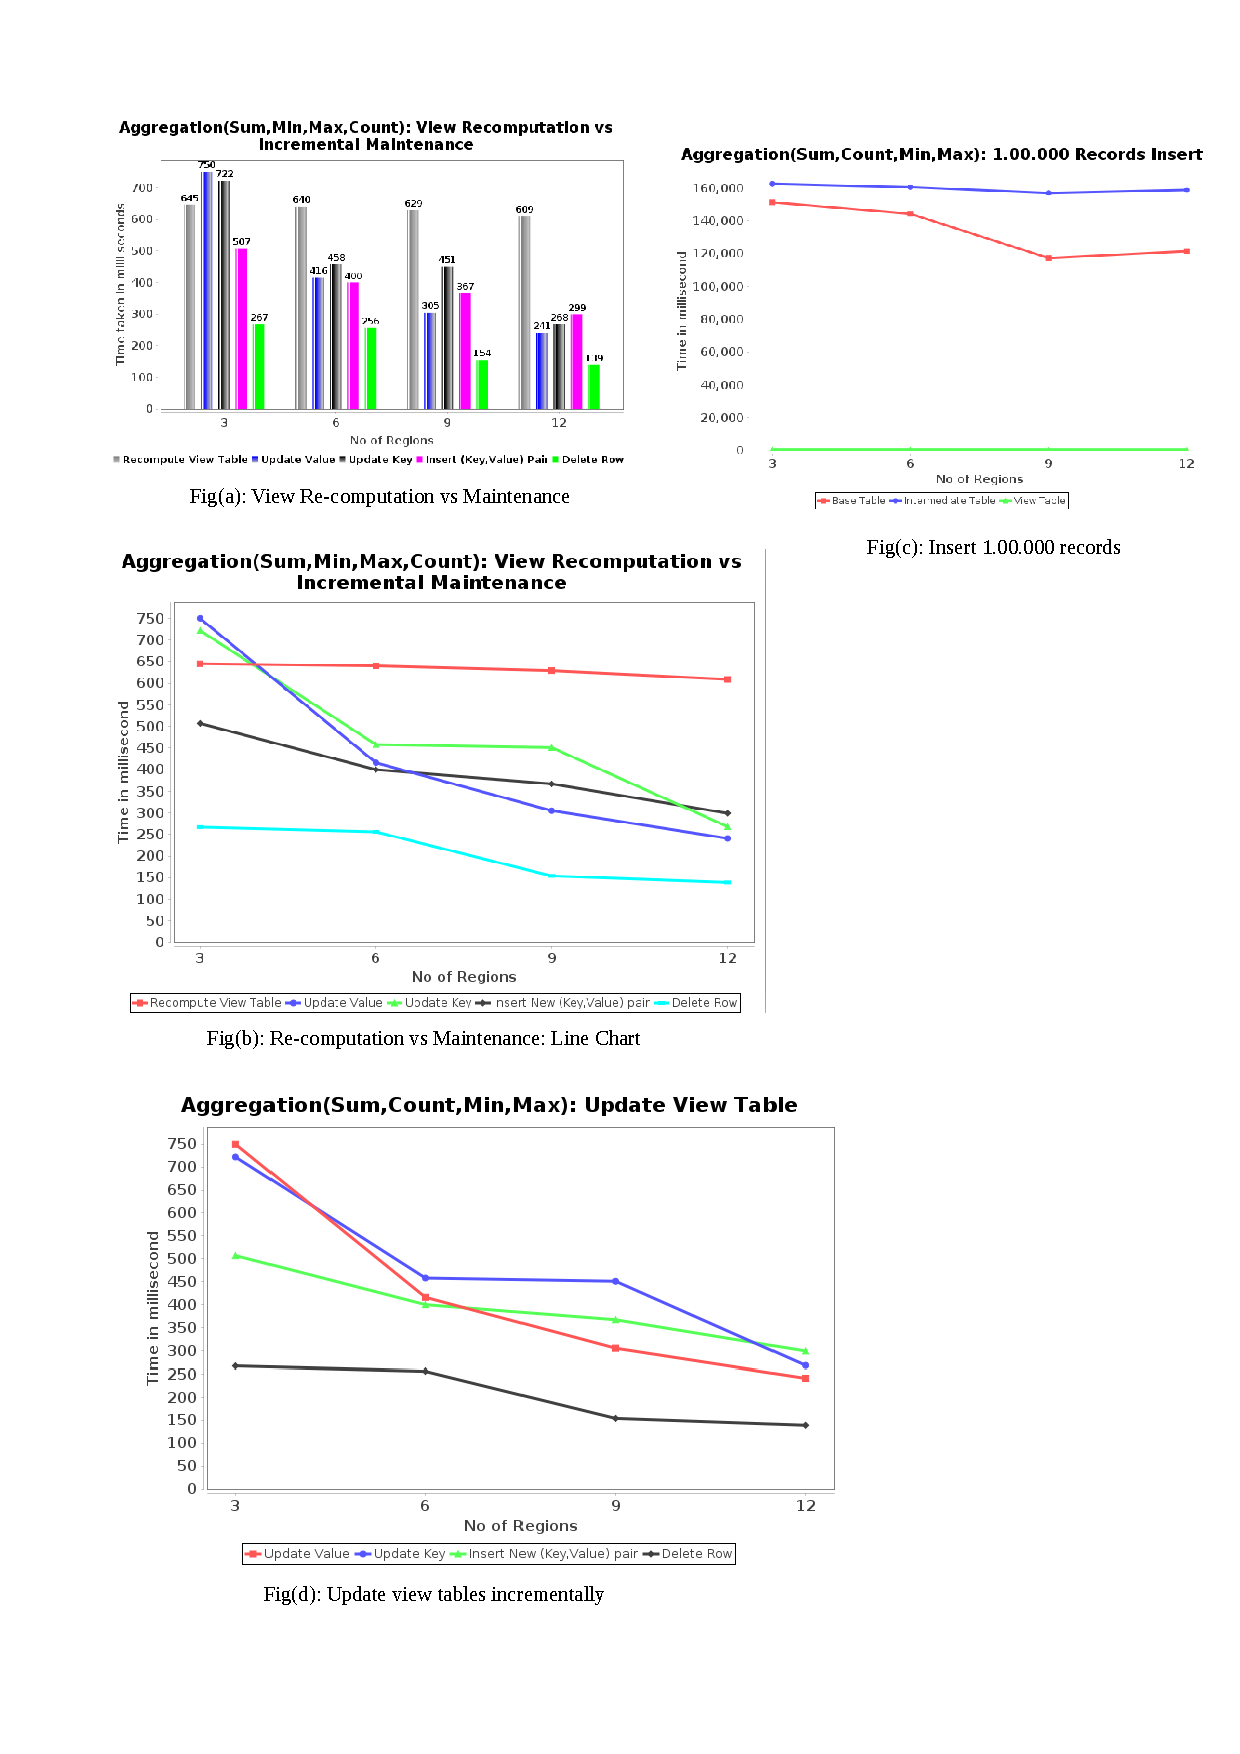
\includegraphics[width=\linewidth]{Aggr_exp_dist}
	\caption{Aggregation Experiment Distributed}
	\label{sec:AggrExpDist}
	
\end{figure} 
\newpage

From the Fig(a) and Fig(b), we proved that incremental maintenance takes less time than re-computing view table to maintain consistency between base table and view table. The reason for the significant improvement in performance of incremental update over the baseline is due to read-write and recompute overhead. We ran our experiment in distributed cluster environment, from one region per region server to four regions per region server. The reason for this improvement is that the table is split horizontally across all the regions. We implemented $HexStringSplit$ algorithm  to partition the table evenly across all the regions, as a result of which the load is distributed equally among all the regions.


\subsection{Aggregation: Insert Records}
\label{Insert Records Aggr Dist}
In this experiment we wanted to prove that splitting tables in multiple regions across multiple region servers in a cluster also improves the performance. We performed the experiment on a dataset with 100,000 records in a clustered environment. In the first scenario, we had one region in each of the region servers making three regions in total. First we inserted 1.00.000 records and compute intermediate and view table and noted the time take for each operation. We ran same experiment for two, three and four regions per region server and noted time take for each operation to be completed. We plotted a graph and from the Fig(c) in the figure \ref{sec:AggrExpDist}, we proved that having more regions yields to the better performance. The key reason for this performance optimization is having load balancer to evenly distribute load to all the available regions.


\subsection{Aggregation: Update View Table} 
\label{Update View Table Aggr Dist}
In section \ref{Insert Records Aggr Dist}, we proved that we can improve performance if we split our tables in multiple regions across multiple region servers. In this experiment, we wanted to see how it affects the performance if we split $View$ $Table$ in multiple regions across multiple region servers. In the figure \ref{sec:AggrExpDist}, $Fig(d)$, in x-axis we show no. of regions and in y-axis, we show time taken to update view table incrementally in millisecond. We first insert 1.00.000 records in base table and pre-compute view tables accordingly. For each of the operation in base table, we evaluate changes in the view table incrementally and plot the graph. Having equally distributed load among the regions, we proved that we can improve the overall performance.  

\section{Experiment 5 (Join and Aggregation)}
\label{(sec:Join and Aggregation Dist)} 
For $Join$ \& $Aggregation$, we create two base tables as it involves k-kf joins and generate corresponding intermediate and view tables. We insert 2.000 rows in both the base table, apply K-FK joins and calculate sum for K-FK joins and insert result in the view table. We then run experiments to see how we can improve performance as we split our tables in multiple regions across multiple region servers.

\subsection{Join and Aggregation: Compute base tables and view table}
\label{Join and Aggregation: Compute base tables and view table}
In this experiment, we insert 2.000 records in both base tables. We then apply K-FK join and compute intermediate table and view table. We calculate sum based on the result of K-FK join and store it in the view table. In such case, we don't know the no. of rows generated based on the K-FK join so we analyze no. of rows generated as a benchmark for rest of the experiments. We pre-split tables into multiple regions and run the experiment for each of the scenarios. Based on the K-FK join on the base tables, we generated 1.53.000-1.55.000 rows in the view table.

 %First we run this experiment in a single region and see the number of rows generated in the view table after applying K-FK joins. We run this experiment for 2, 3 and 4 regions and split our tables accordingly. In the figure \ref{sec:JoinAggrExpStandalone}, Fig(a) shows the graph of no. of records inserted in view tables. We use this statistics for running other sub-experiments.

\subsection{Join and Aggregation: View Re-computation vs Maintenance}
\label{Join and Aggregation: View Re-computation vs Maintenance Distributed}

To evaluate performance in View Re-computation vs Maintenance, we first create two base tables with 2.000 rows and generate corresponding intermediate and view tables. The view table consists of a aggregation (sum) of K-FK join between the two base table data. We wanted to show that incrementally maintaining our view tables yields in significant improvement on the performance. To prove our assumption, we ran our experiment on the basis of rows generated in section \ref{Join and Aggregation: Compute base tables and view table}. From the Figure \ref{sec:JoinAggrExpDist}, Fig(a) shows time taken to re-compute view table vs time taken to incrementally update view table. Here we observe that incremental method yields up to 98\% improvement over the baseline. The reason for the significant improvement in performance of incremental update over the baseline is due to read-write and recompute overhead. In the re-compute method, we need to read the whole base table and
reconstruct the view table. However, in the incremental method, we do not reconstruct the view table but only update the rows that are affected by the operation on the base table. 


\subsection{Join and Aggregation: Insert Records}
\label{Join and Aggregation: Insert Records Distributed}
In this experiment we first create two base tables with 2.000 rows and generate corresponding intermediate and view tables. The view table consists of aggregation(sum) of K-FK join between the two base table data. In this experiment we wanted to prove that evenly distributing load to multiple regions can yield to a significant performance optimization. For that we evenly distributed base tables, intermediate table and a view table across all the regions on a multiple region servers.  
To prove our assumption, we ran our experiment on the basis of rows generated in section \ref{Join and Aggregation: Compute base tables and view table}. In the x-axis, we showed no. of regions and in y-axis we showed time taken in millisecond to complete the operation. From the figure \ref{sec:JoinAggrExpDist}, Fig(c), we can see that splitting tables into multiple regions and using load balancing can significantly reduce operation time.

\subsection{Join and Aggregation: Update View Table} 
\label{Join and Aggr: Update View Table Distributed}

In section \ref{Join and Aggregation: Insert Records Distributed},  we proved that we can improve optimization if we split our tables in multiple regions across multiple region servers. In this experiment, we wanted to see how it affects the performance if we split $View$ $Table$ across multiple regions. For that, we split $View$ $Table$ across multiple regions and ran this experiment. 
In the figure \ref{sec:JoinAggrExpDist}, $Fig(d)$, we show time taken to update view table incrementally in millisecond. In the first experiment set, we pre-split $View$ $Table$ into three regions. Then we evaluate time taken to update view table incrementally for each of the update operations on the base table. We run this experiment again after pre-splitting $view$ $table$ into multiple regions and evaluate time taken to update view table incrementally. From the figure \ref{sec:JoinAggrExpDist}, $Fig(d)$, we again proved that the more table is split into more no. of regions, the less time is required to update view table incrementally. 

\section{Experiment 6 (Join and Selection)}
\label{(sec:Join and Selection Exp Distributed)} 
For $Join$ \& $Selection$, we create two base tables as it also involves K-FK joins, an intermediate table and a view table. We insert 3.000 rows in both the base table, apply K-FK joins and select values for those joins and insert result in the view table. We then run experiments to see how we can improve performance as we split our tables across multiple regions.

\subsection{Join and Selection: Compute base tables and view tables}
\label{Join and Selection: Compute base tables and view table}
In this experiment, we insert 2.000 records in both base tables. We then apply K-FK join and compute intermediate table and view table. We then select values based on the result of K-FK join and store it in the view table. In such case, we don't know the no. of rows generated based on the K-FK join so we analyze no. of rows generated as a benchmark for rest of the experiments. We pre-split tables into multiple regions and run the experiment for each of the scenarios. Based on the K-FK join on the base tables, we generated 1.53.000-1.54.000 rows in the view table.

\subsection{Join and Selection: View Re-computation vs Maintenance}
\label{Join and Selection: View Re-computation vs Maintenance Distributed}

To evaluate performance in View Re-computation vs Maintenance, we first create two base tables with 2.000 rows and generate corresponding intermediate and view tables. The view table consists of a selection of K-FK join between the two base table data. We wanted to show that incrementally maintaining our view tables yields in significant improvement on the performance. To prove our assumption, we ran our experiment on the basis of rows generated in section \ref{Join and Selection: Compute base tables and view table}. From the Figure \ref{sec:JoinSelExpDist}, Fig(a) shows time taken to re-compute view table vs time taken to incrementally update view table. Here we observe that incremental method yields up to 98\% improvement over the baseline. The reason for the significant improvement in performance of incremental update over the baseline is due to read-write and recompute overhead. In the re-compute method, we need to read the whole base table and
reconstruct the view table. However, in the incremental method, we do not reconstruct the view table but only update the rows that are affected by the operation on the base table. 

\begin{figure}
	\centering
	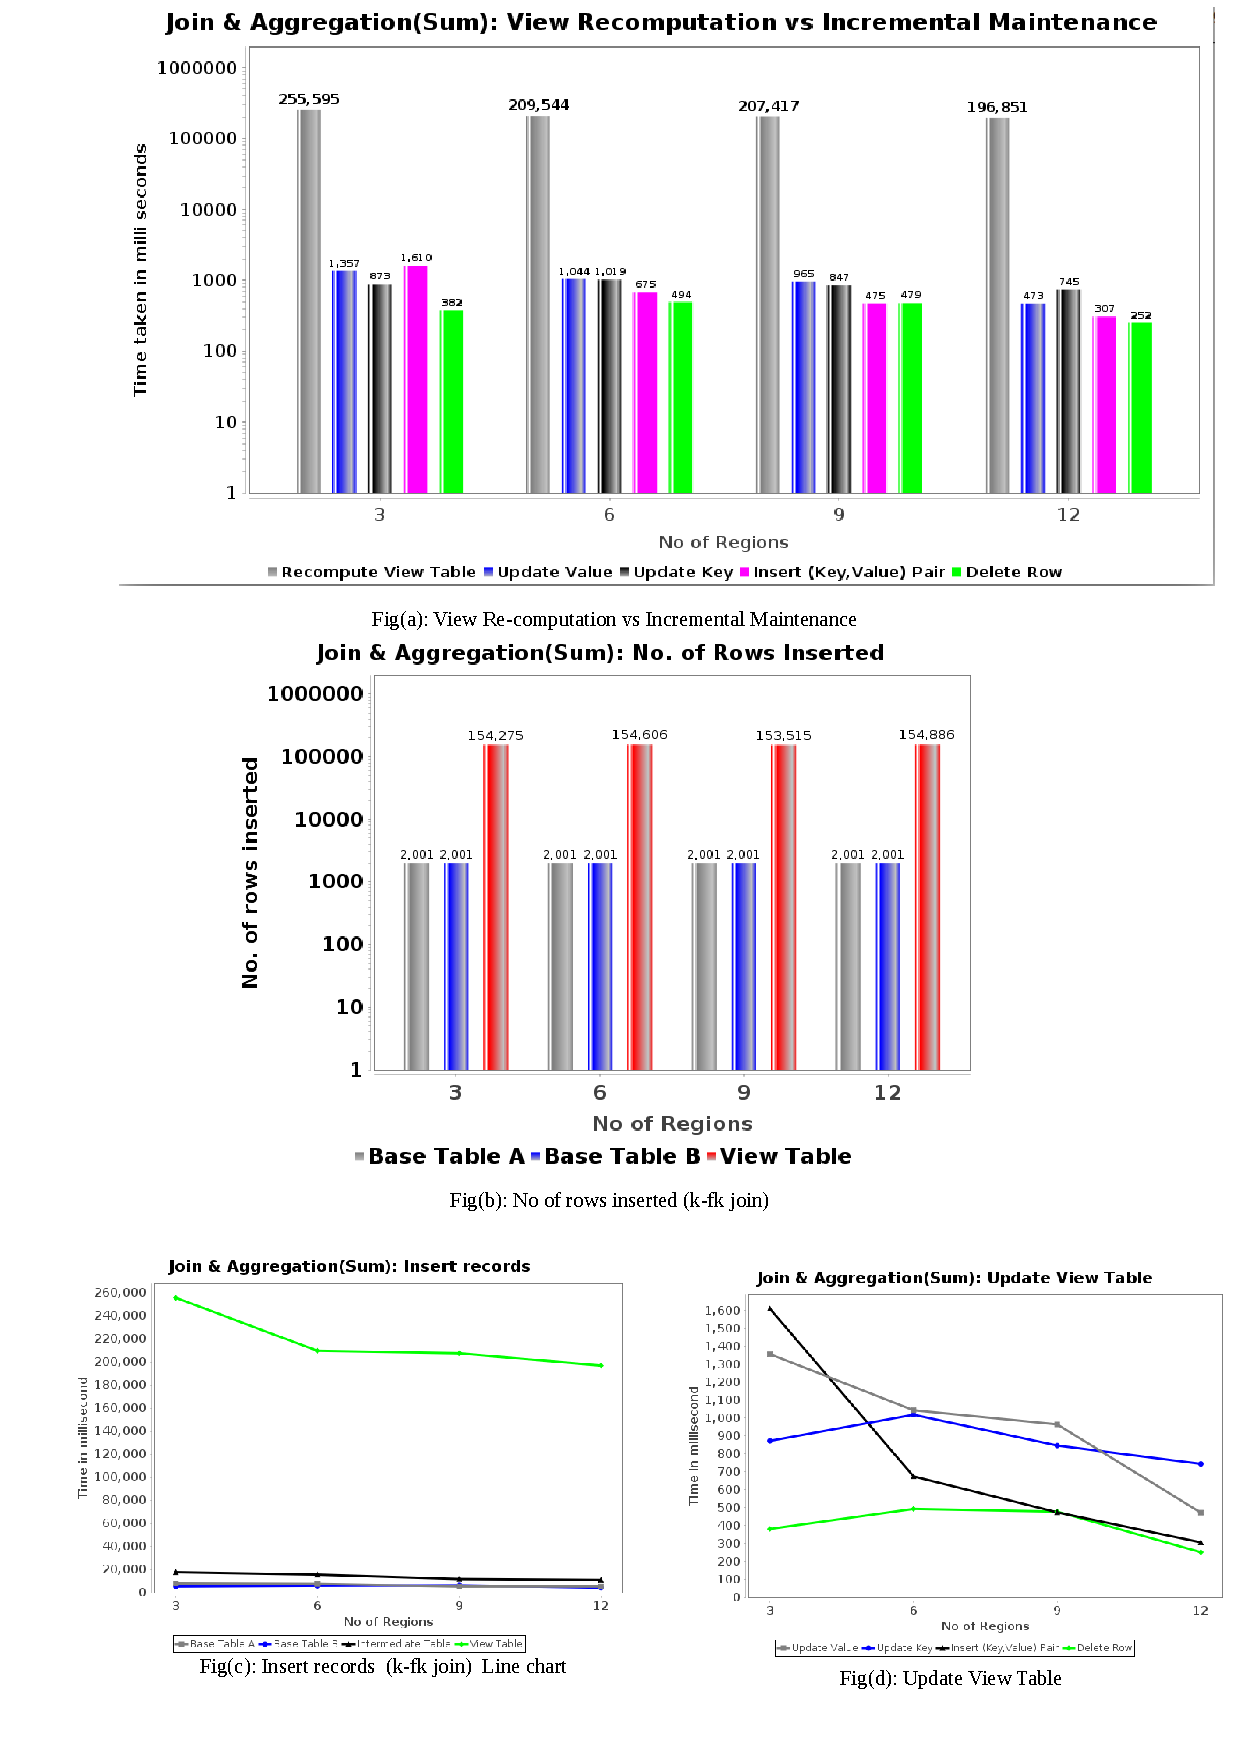
\includegraphics[width=\linewidth]{JoinAndAggr_exp_dist}
	\caption{Join and Aggregation Experiment Distributed}
	\label{sec:JoinAggrExpDist}
	
\end{figure} 
\newpage



\subsection{Join and Selection: Insert Records}
\label{Join and Selection: Insert Records Distributed}

In this experiment we first create two base tables with 2.000 rows and generate corresponding intermediate and view tables. The view table consists of selection of K-FK join between the two base table data. In this experiment we wanted to prove that evenly distributing load to multiple regions can yield to a significant performance optimization. For that we evenly distributed base tables, intermediate table and a view table across all the regions on a multiple region servers.  
To prove our assumption, we ran our experiment on the basis of rows generated in section \ref{Join and Selection: Compute base tables and view table}. In the x-axis, we showed no. of regions and in y-axis we showed time taken in millisecond to complete the operation. From the figure \ref{sec:JoinSelExpDist}, Fig(c), we can see that splitting tables into multiple regions and using load balancing can significantly reduce operation time.

\subsection{Join and Selection: Update View Table} 
\label{Join and Sel: Update View Table Distributed}

In section \ref{Join and Selection: Insert Records Distributed},  we proved that we can improve optimization if we split our tables in multiple regions across multiple region servers. In this experiment, we wanted to see how it affects the performance if we split $View$ $Table$ across multiple regions. For that, we split $View$ $Table$ across multiple regions and ran this experiment. 
In the figure \ref{sec:JoinSelExpDist}, $Fig(d)$, we show time taken to update view table incrementally in millisecond. In the first experiment set, we pre-split $View$ $Table$ into three regions. Then we evaluate time taken to update view table incrementally for each of the update operations on the base table. We run this experiment again after pre-splitting $view$ $table$ into multiple regions and evaluate time taken to update view table incrementally. From the figure \ref{sec:JoinSelExpDist}, $Fig(d)$, we again proved that the more table is split into more no. of regions, the less time is required to update view table incrementally. 

\begin{figure}
	\centering
	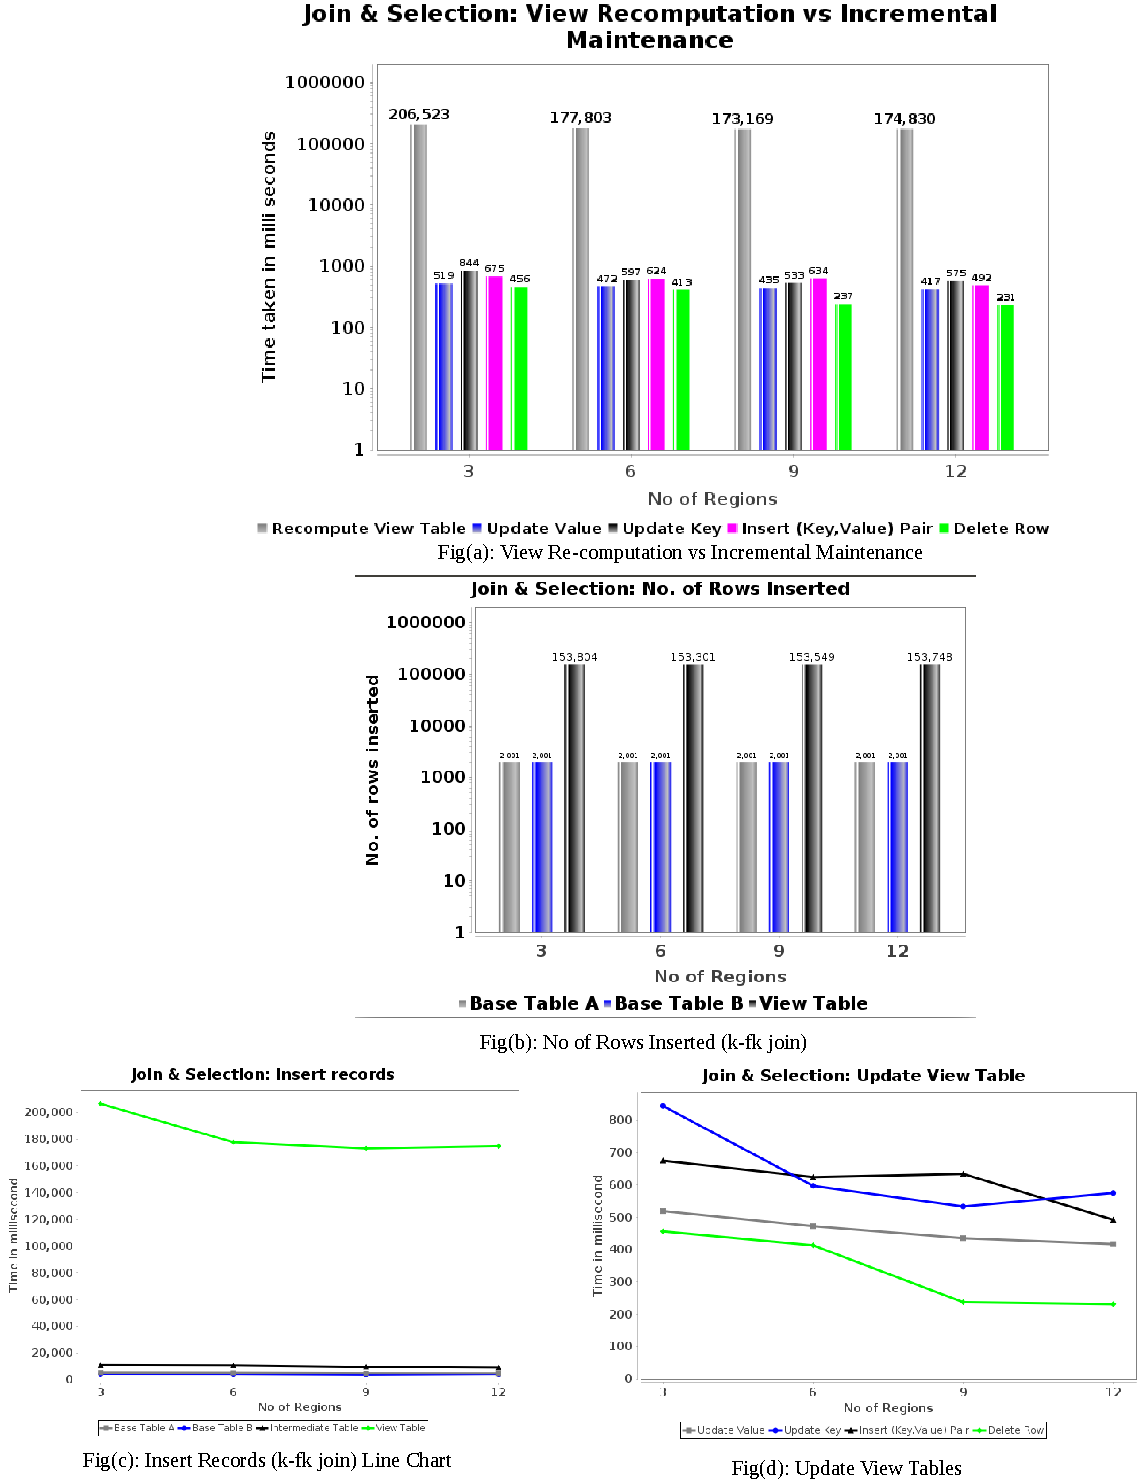
\includegraphics[width=\linewidth]{JoinSel_exp_dist}
	\caption{Join and Selection Experiment Distributed}
	\label{sec:JoinSelExpDist}
	
\end{figure} 


\chapter{Conclusion}
\label{Conclusion}
We have presented an approach to maintain consistency between base table and view table incrementally using HBase Coprocessor. We have provided a solution for incremental maintenance of view table without re-computing view table for every updates on base table. We managed to load coprocessor in the base table. For every updates on the base table, we managed to trigger required updates on the view table using coprocessor and apply them in the view table. This solution addressed the problem of having read-write overhead for re-computing view table even for small changes in the base table. We introduced an intermediate table where all the values for a particular key were plotted in a single row. So for every update for a particular key on base table, we only need to scan one row in intermediate table to determine updates required in view table. This architecture overcomes read overhead i.e. we only need to scan one particular row instead of scanning whole base table to determine changes required for view table. As we overcome read-write overhead, we managed to improve performance of the system up to 98\% in the best case scenario. To prove our hypothesis, we ran experiments on different datasets ranging from 10.000 rows to 2.50.000 rows. We tested our solution for different view types namely $Sum$, $Count$, $Min$, $Max$ and $K-FK$ $join$ views. We performed several experiments both on pseudo-distributed mode and fully distributed mode. In both environments, we were able to optimize performance significantly. 


\chapter{Future Work}
\label{Future Work}
We have used HBase Client API and HBase shell to read and write data into the HBase tables. Many of us are more familiar with SQL queries, we also can use SQL like queries to read from and write into hbase tables. Apache Spark provides Spark DataFrame DataSource which helps to integrate Spark SQL with HBase and write SQL alike queries to read and write into hbase tables. Apache Hive also provides HiveQL for SQL like query to the HBase tables. 
\newline
We ran our experiment in a laptop with two virtual machine acting as a multi-node cluster. It would be more interesting to run our experiment on cluster of more than 20 nodes with a  dataset of few hundred millions records and see the results.


		% ---------------------------------------------------------------------------
		%
		% Appendix
		%
		% ---------------------------------------------------------------------------
		
		\part*{Appendix}
		\addcontentsline{toc}{part}{Appendix}
		
		\appendix %---------------------------------------
		
		%\chapter{Components}
%\section{Detailed Validation Results}
\label{chapter:Components}

\section{VM Master}


\textbf{Interface}

\begin{enumerate}
	\item Ingoing
	\begin{itemize}
		\item $viewManagerAdded$
		\item $viewManagerAssigned$
		\item $viewManagerRemoved$
		\item $viewManagerWithdrawn$
		\item $viewManagerReassigned$
		\item $regionServerAdded$
		\item $regionServerRemoved$
		\item $callLastCommitedUpdate$
	\end{itemize}
	\item Outgoing
	\begin{itemize}
		\item $createZookeperNode$
		\item $assignViewManager$
		\item $reassignViewManager$
		\item $withdrawViewManager$
		\item $removeViewManager$
		\item $replayWriteAheadLog$

	\end{itemize}
\end{enumerate}


\textbf{Subcomponents}

\begin{enumerate}
	\item $VM\:Master\:Controller$
	\item $Event\:Processor$
	\item $Load\:Balancer$
	\item $Recover\:Manager$
	\item $Component\:Controller$
\end{enumerate}
\newpage
\begin{figure}[h!] 
  \centering
    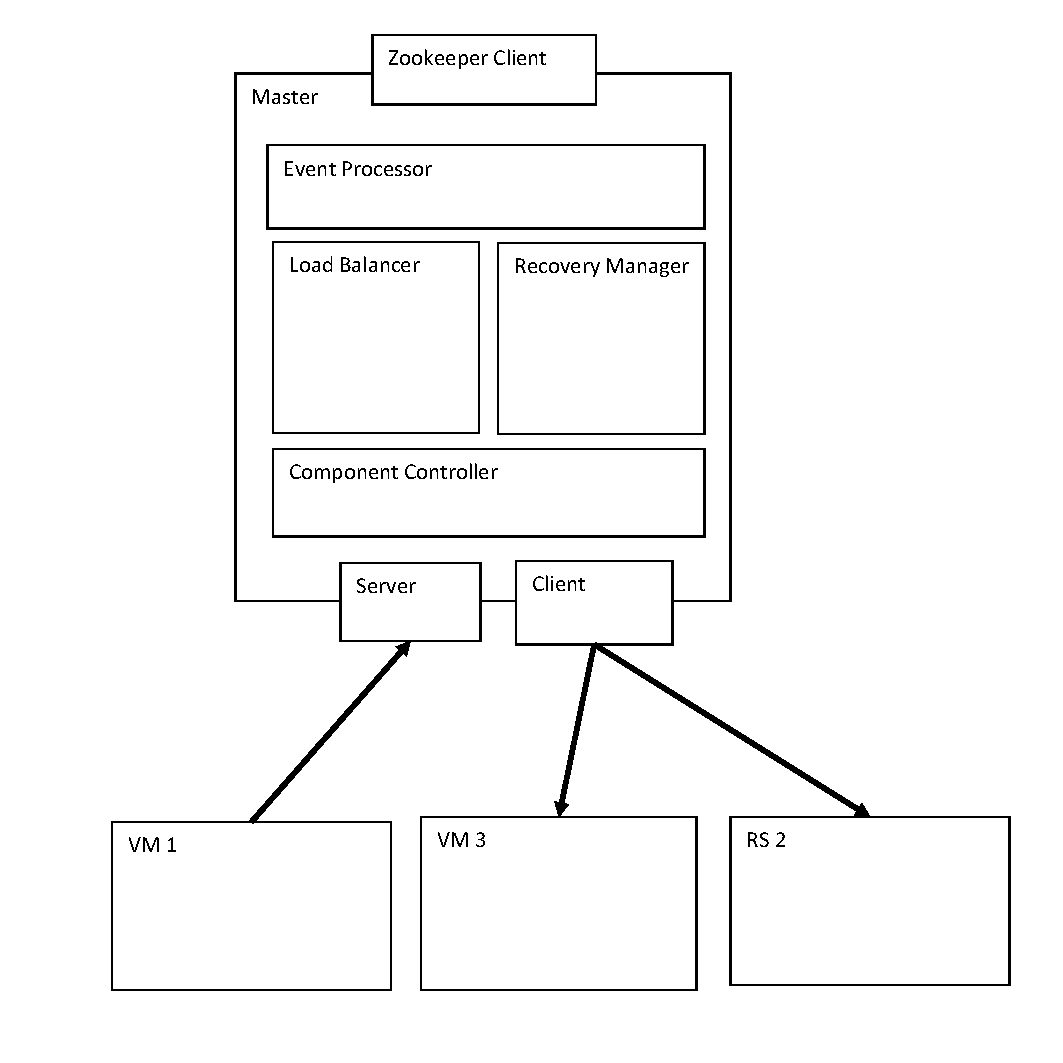
\includegraphics[scale=0.8]{figures/Master}
    \caption{Master}
    \label{fig:master}
\end{figure}

\newpage

\section{VM Region Server}

\textbf{Interface}

\begin{enumerate}
	\item Ingoing
	\begin{itemize}
		\item $put, get, delete$
		\item $assignViewManager$
		\item $withdrawViewManager$
		\item $replayWriteAheadLog$
		\item $statusReportViewManager$
	\end{itemize}
	\item Outgoing
	\begin{itemize}
		\item $createZookeeperNode$
		\item $sendUpdate$
		\item $sendStatusReport$
	\end{itemize}
\end{enumerate}


\textbf{Subcomponents}

\begin{enumerate}
	\item $HBase\:Region\:Server$
	\item $RS\:Controller$
	\item $Write\:Ahead\:Log$
	\item $WAL\:Reader$
	\item $Update\:Assigner$
	\item $Update\:Distributor$
\end{enumerate}

\newpage
\begin{figure}[h!]
  
  \centering
    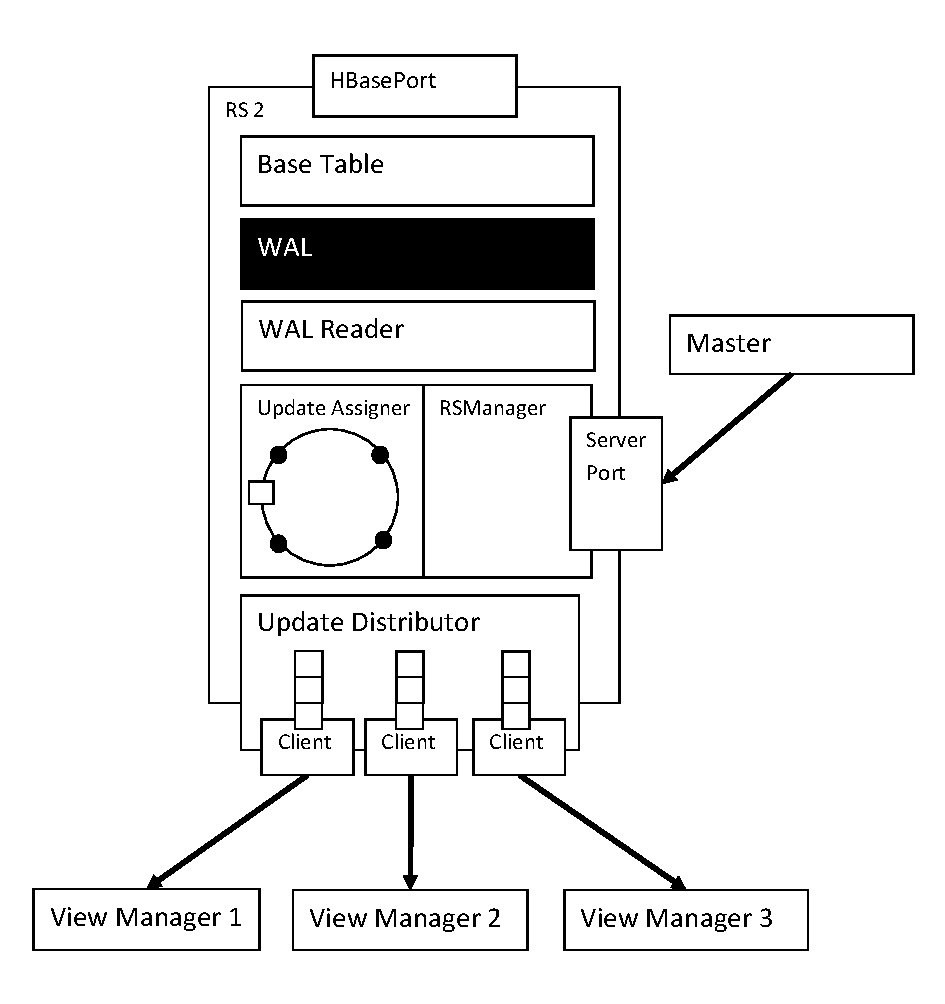
\includegraphics[scale=0.8]{figures/RegionServer}
    \caption{Region Server}
    \label{fig:regionserverAppendix}
\end{figure}
\newpage

\section{View Manager}



\textbf{Interface}

\begin{enumerate}
	\item Ingoing
	\begin{itemize}
		\item $receiveUpdate$
		\item $assignViewManager$
		\item $withdrawViewManager$
		\item $reassignViewManager$
		\item $removeViewManager$
		\item $callLastCommitedUpdate$
	\end{itemize}
	\item Outgoing
	\begin{itemize}
		\item $createZookeeperNode$
		\item $shutdownViewManager$
		\item $assignViewManager$
		\item $withdrawViewManager$
		\item $getViewDefinitions$
		\item $sendStatusReport$

	\end{itemize}
\end{enumerate}

\textbf{Subcomponents}

\begin{enumerate}
	\item $VM\:Controller$
	\item $Pre-Processor$
	\item $Processor$
	\item $Commit\:Log$
\end{enumerate}

\newpage

\begin{figure}[h!]
  
  \centering
    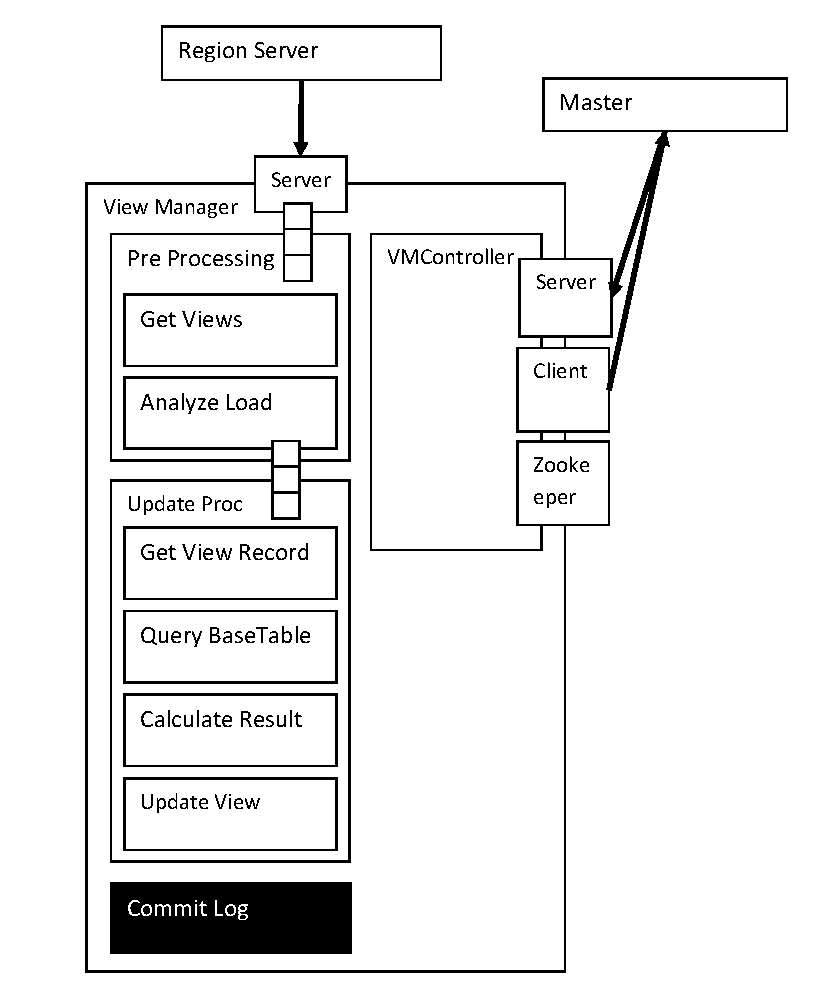
\includegraphics[width=\linewidth]{figures/ViewManager}
    \caption{View Manager}
    \label{fig:viewmanager}
\end{figure}
\newpage



\chapter{System Operations}
\label{chapter:Sytem Operations}


\section{Add View Manager}
\begin{figure}[h!]
  \centering
    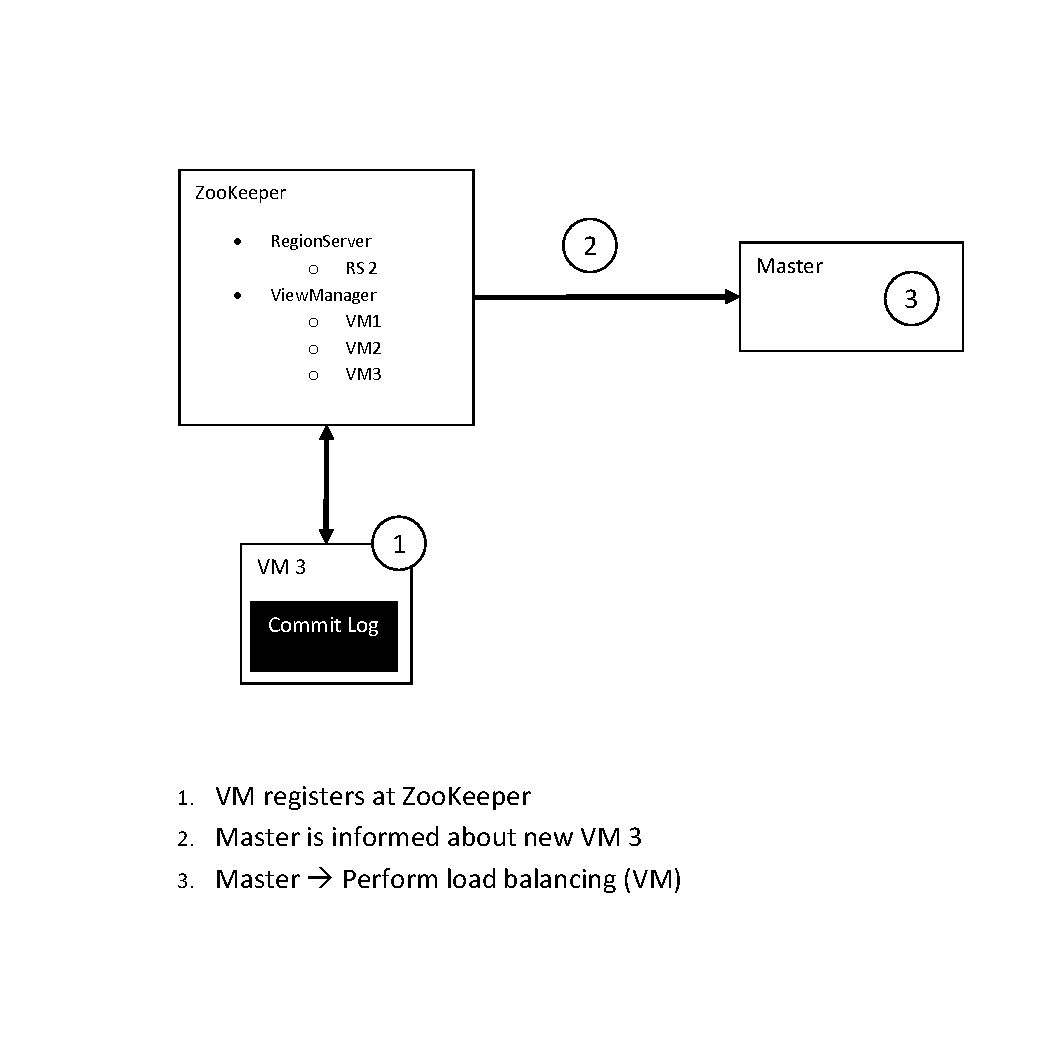
\includegraphics[scale=0.8]{figures/SO_AddViewManager}
    \caption{Add View Manager}
    \label{fig:addviewmanager}
\end{figure}
\newpage

\section{Assign View Manager}
\begin{figure}[h!]
  \centering
    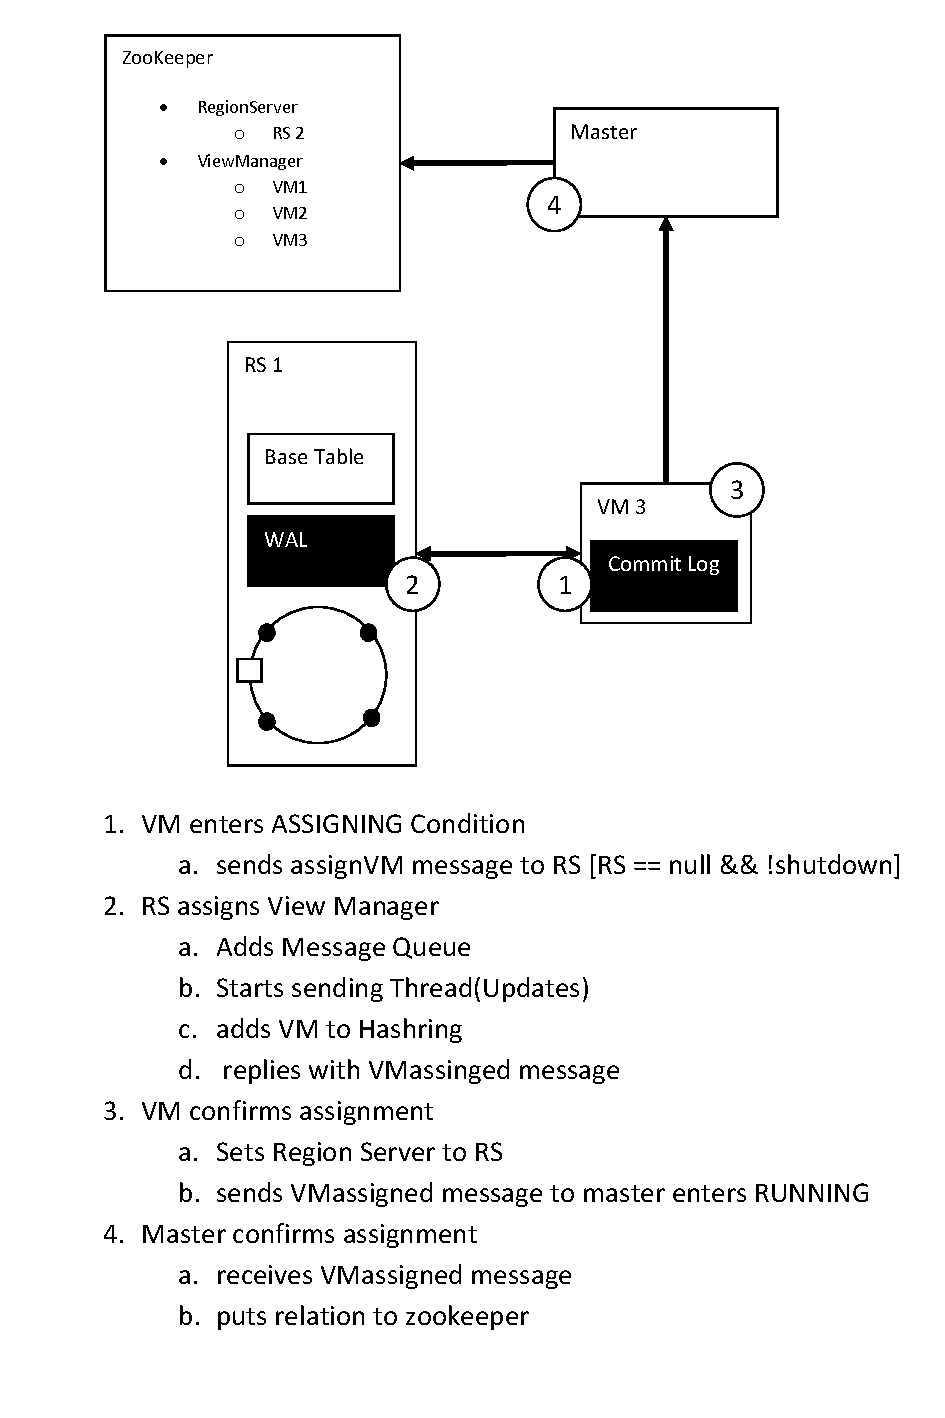
\includegraphics[scale=0.8]{figures/SO_AssignViewManager}
     \caption{Assign View Manager}
    \label{fig:assignviewmanager}
\end{figure}
\newpage

\section{Withdraw View Manager}
\begin{figure}[h!]
  \centering
    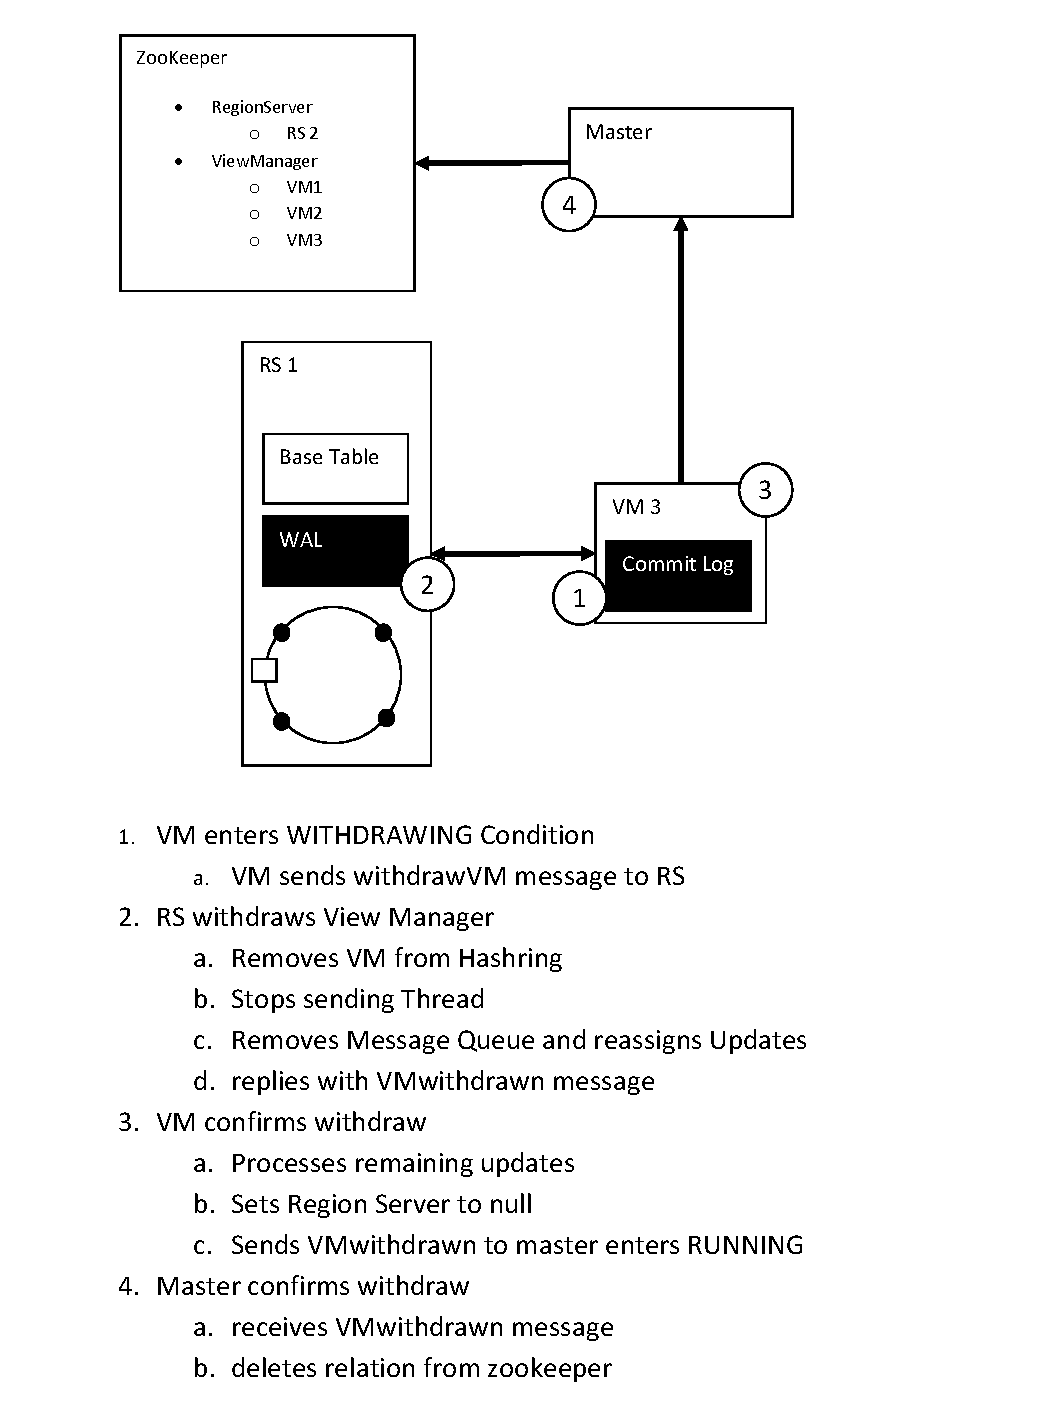
\includegraphics[scale=0.8]{figures/SO_WithdrawViewManager}
     \caption{Withdraw View Manager}
    \label{fig:withdrawviewmanager}
\end{figure}
\newpage
\section{Reassign View Manager}
\begin{figure}[h!]
  \centering
    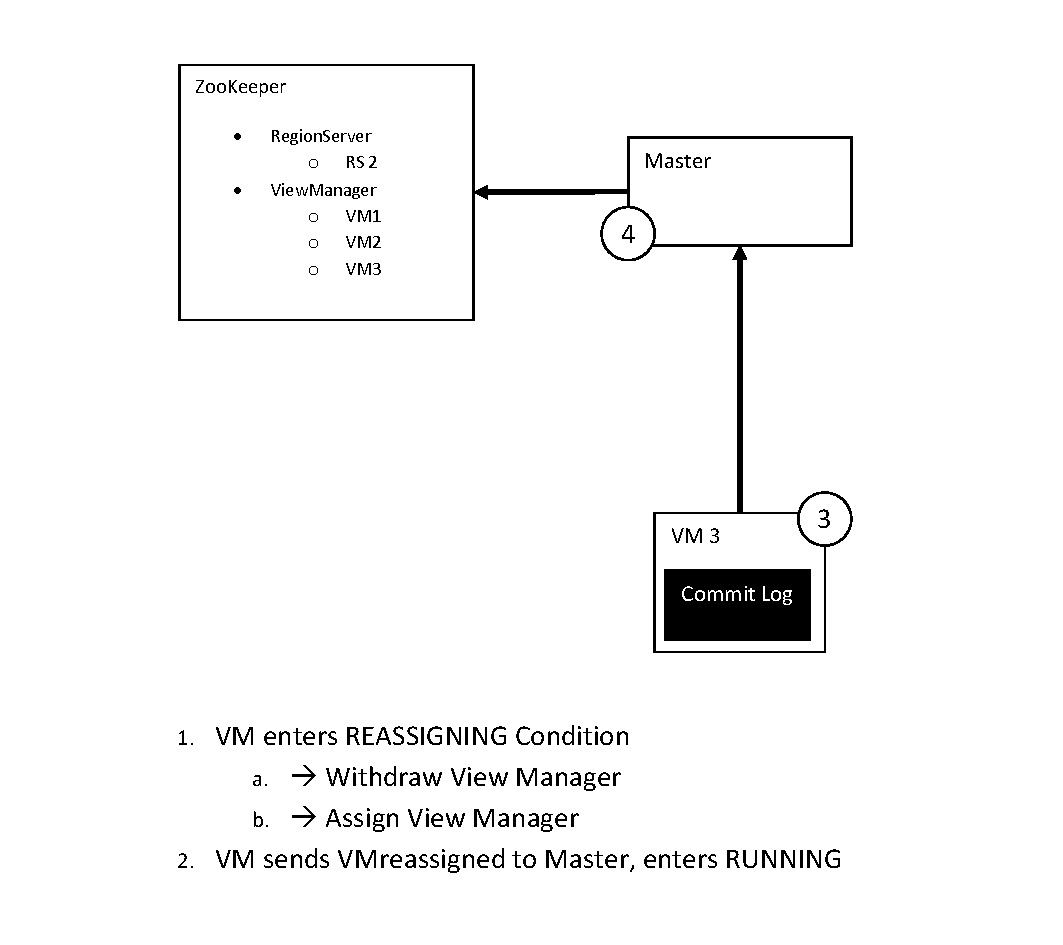
\includegraphics[scale=0.8]{figures/SO_ReassignViewManager}
     \caption{Reassign View Manager}
    \label{fig:reassignviewmanager}
\end{figure}

\newpage

\section{View Manager Crash}
\begin{figure}[h!]
  \centering
    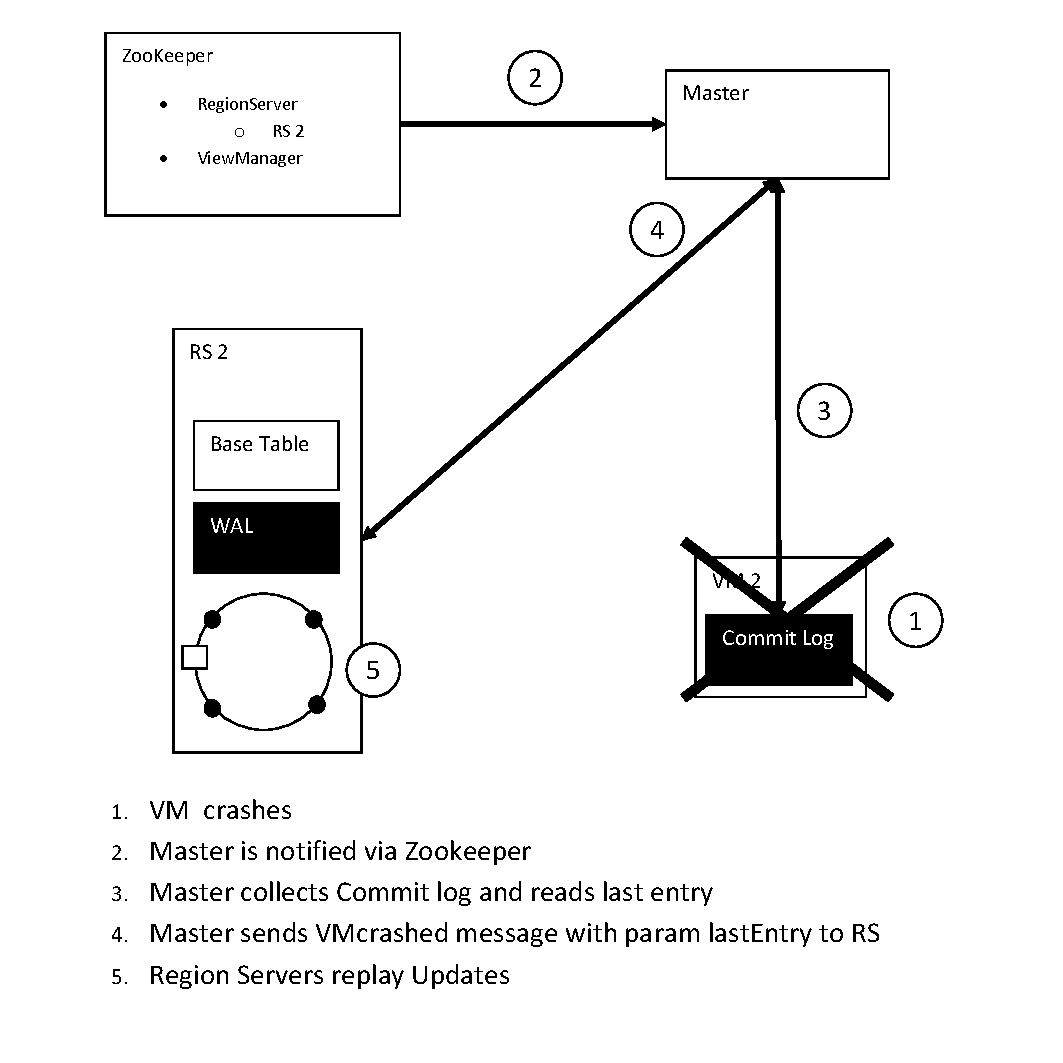
\includegraphics[scale=0.8]{figures/SO_ViewManagerCrash}
     \caption{View Manager Crash}
    \label{fig:so_viewmanagercrash}
\end{figure}
\newpage

\section{Add Region Server}
\begin{figure}[h!]
  \centering
    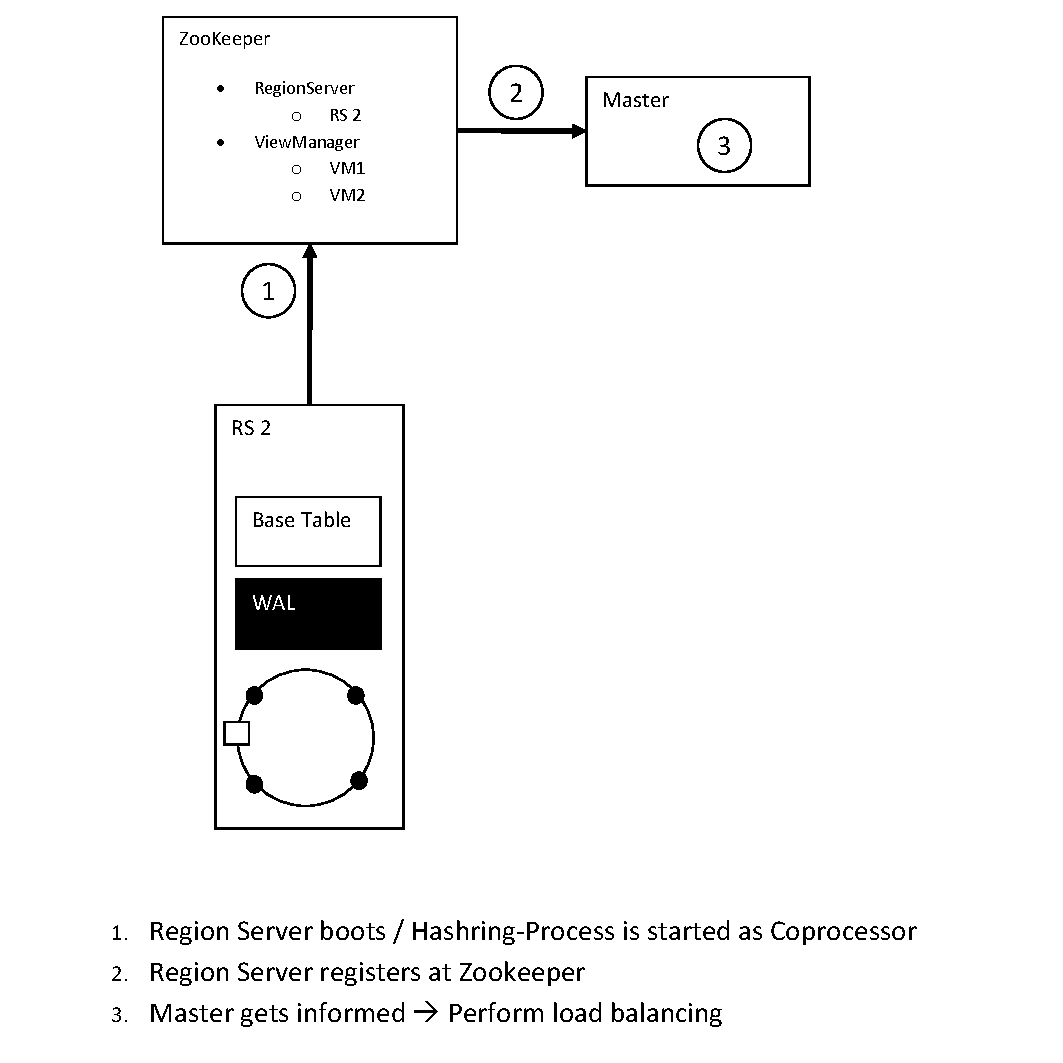
\includegraphics[scale=0.8]{figures/SO_AddRegionServer}
     \caption{Add Region Server}
    \label{fig:addregionserver}
\end{figure}
\newpage

\section{Region Server Crash}
\begin{figure}[h!]
  \centering
    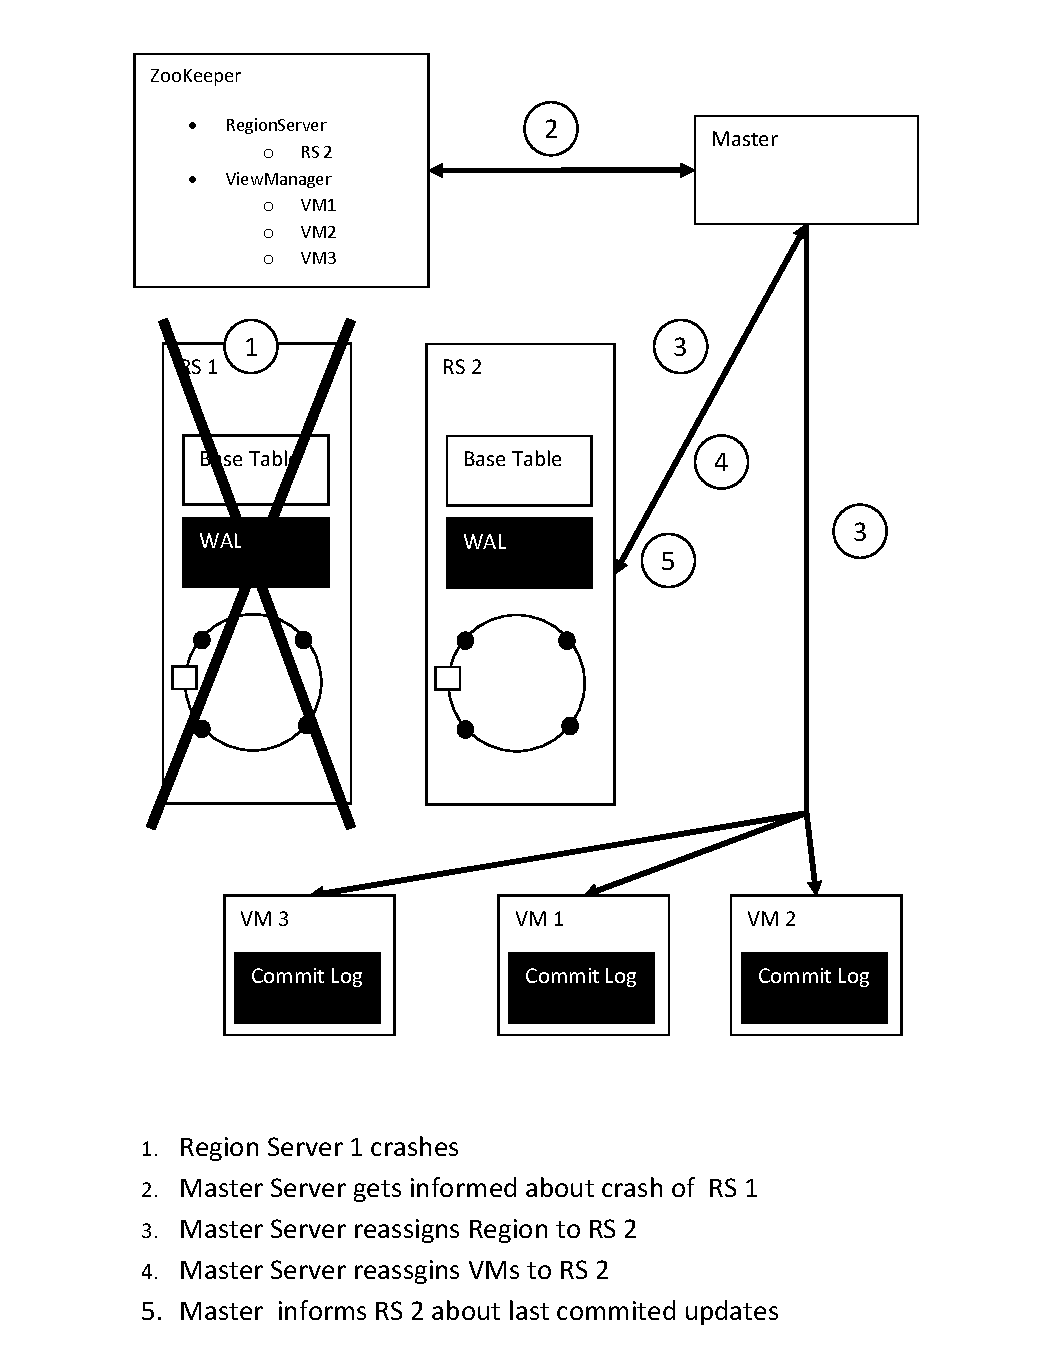
\includegraphics[scale=0.8]{figures/SO_RegionServerCrash}
     \caption{Region Server Crash}
    \label{fig:regionservercrash}
\end{figure}
\newpage

\section{Update Processing}
\begin{figure}[h!]
  
  \centering
    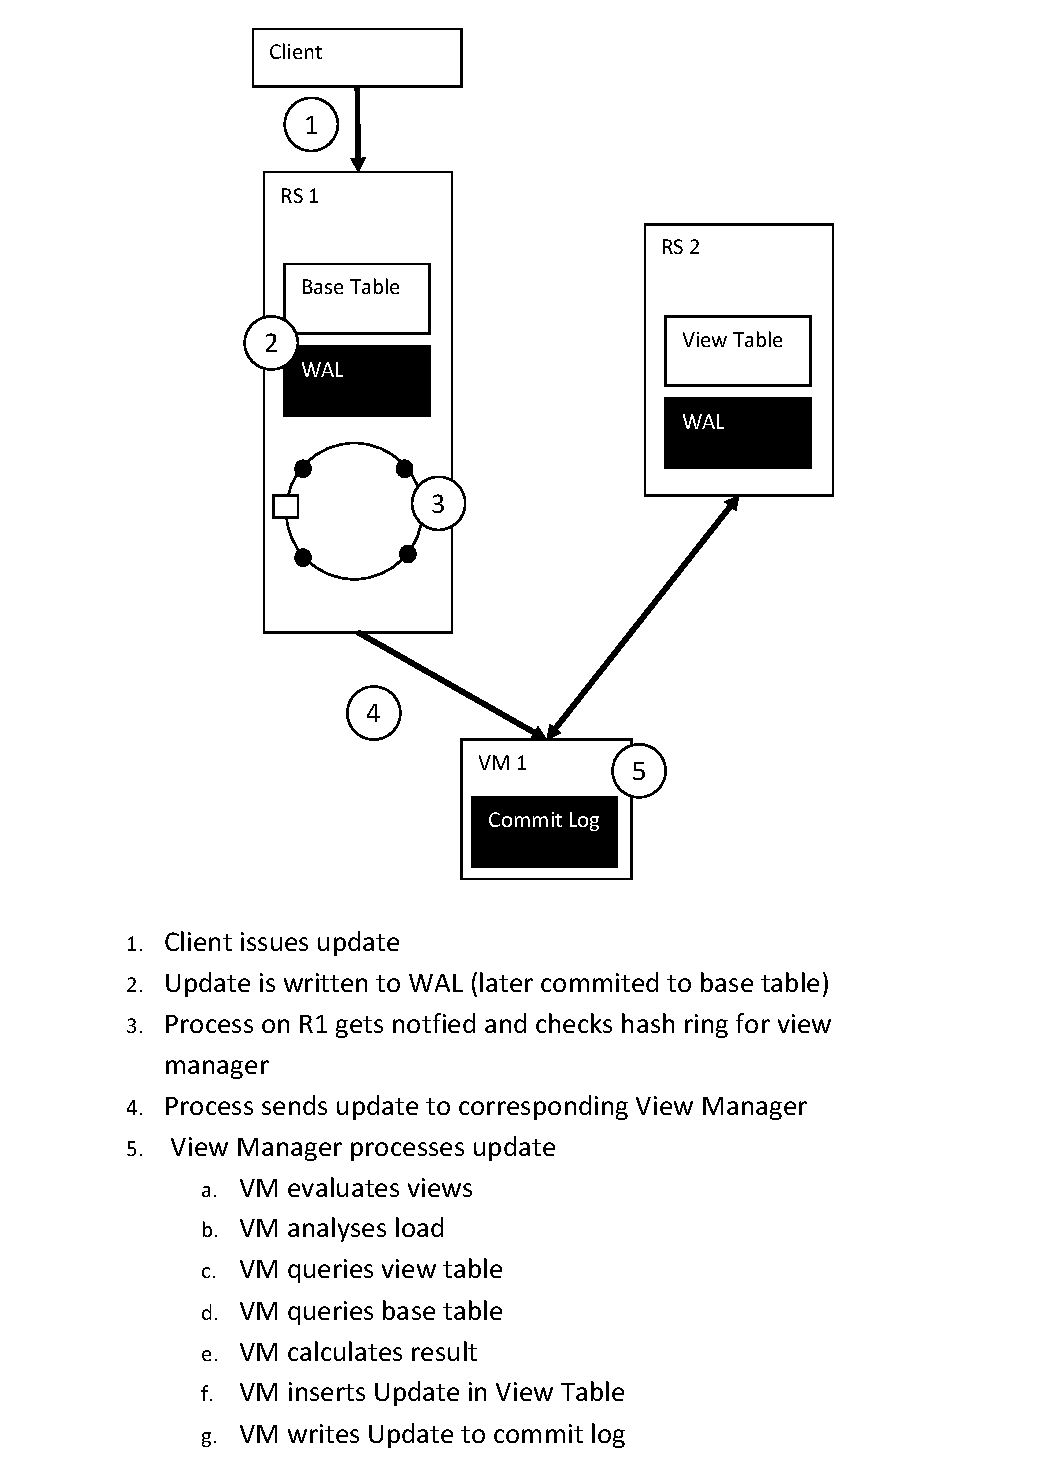
\includegraphics[scale=0.7]{figures/SO_UpdateProcessing}
    \caption{Update Path}
    \label{fig:updatepath}
\end{figure}

\newpage
\section{Status Reports}
\begin{figure}[h!]
  
  \centering
    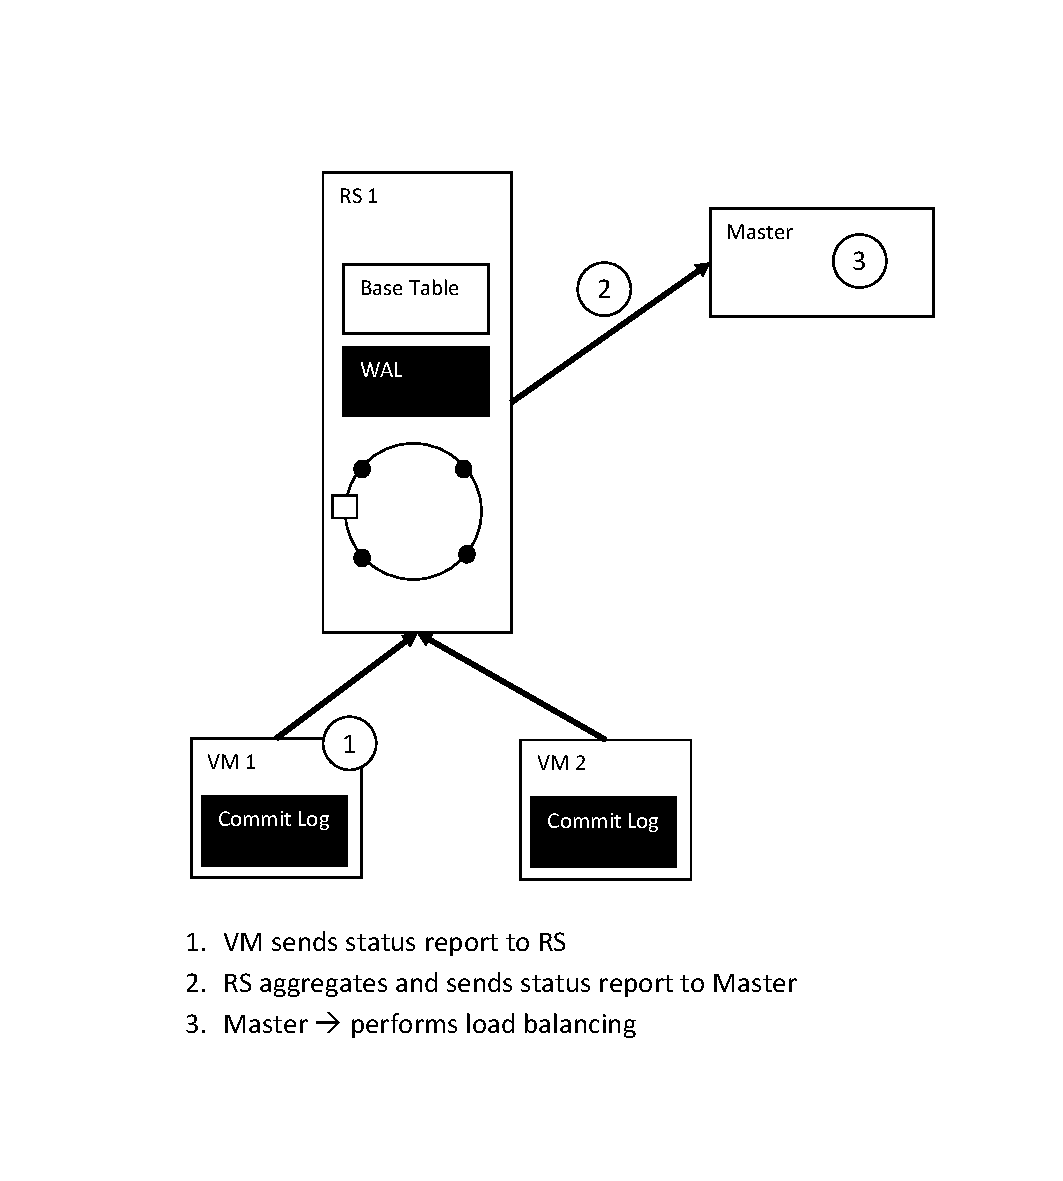
\includegraphics[width=\linewidth]{figures/SO_StatusReports}
    \caption{Status Reports}
    \label{fig:statusreports}
\end{figure}

\chapter{View Consistency}
\label{chapter:viewconsistencyappendix}


\section{Challenges to consistency}
\begin{figure}[h!]
  \centering
    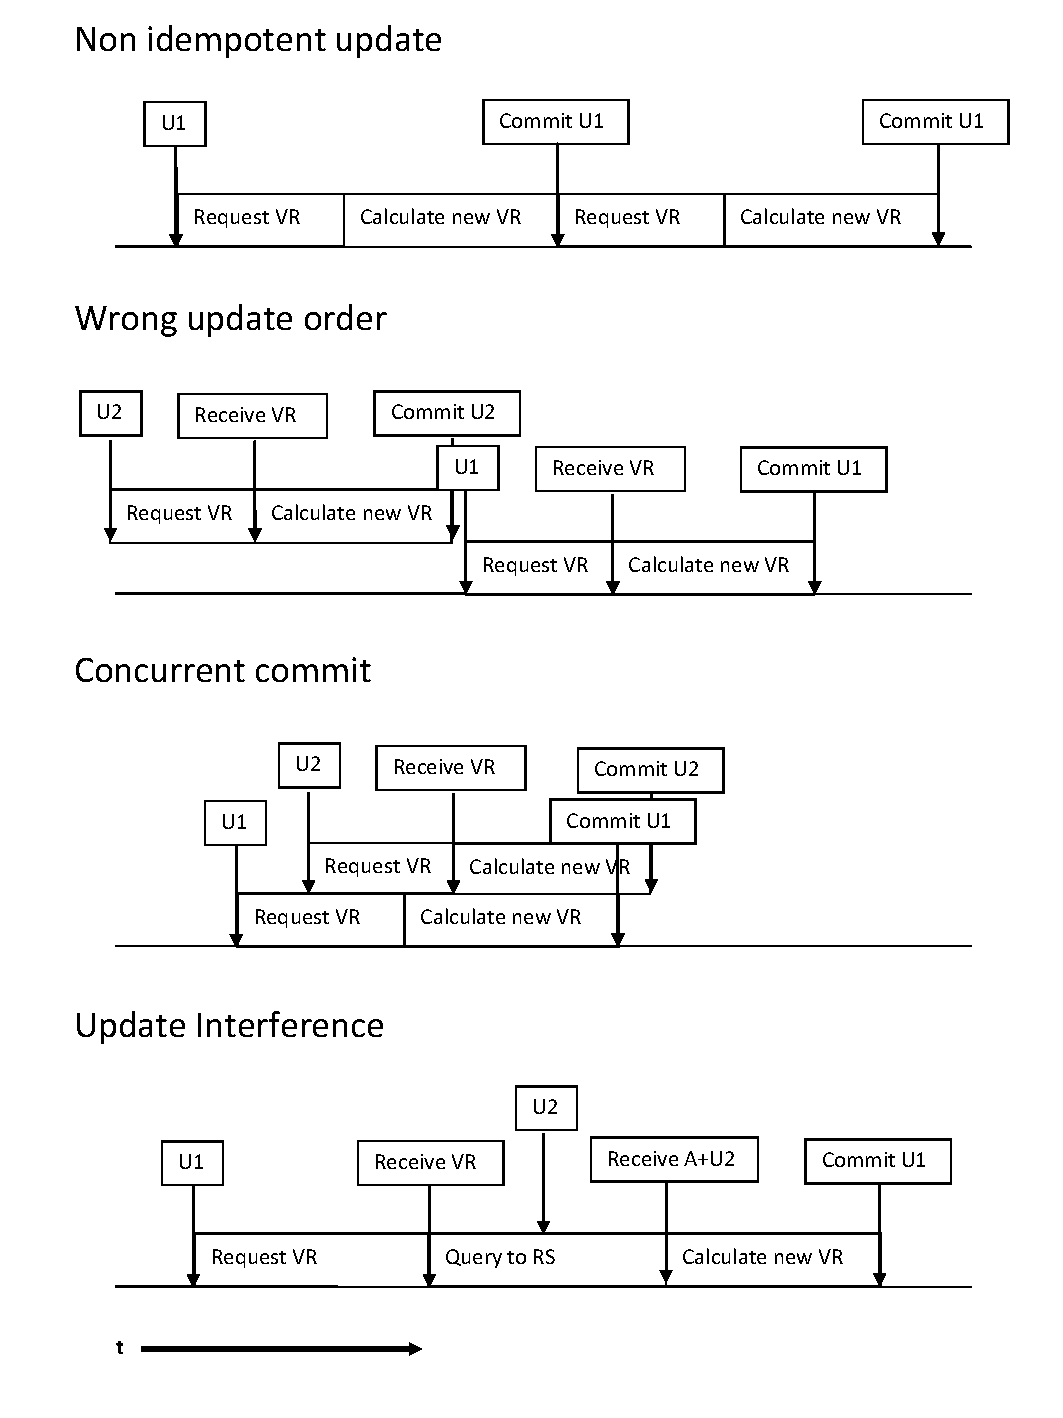
\includegraphics[scale=0.6]{figures/CO_ConsistencyProblems}
     \caption{Consistency threats}
    \label{fig:co_consistencyproblems}
\end{figure}
\newpage

\subsection{Non idempotent view updates}
\begin{figure}[h!]
  \centering
    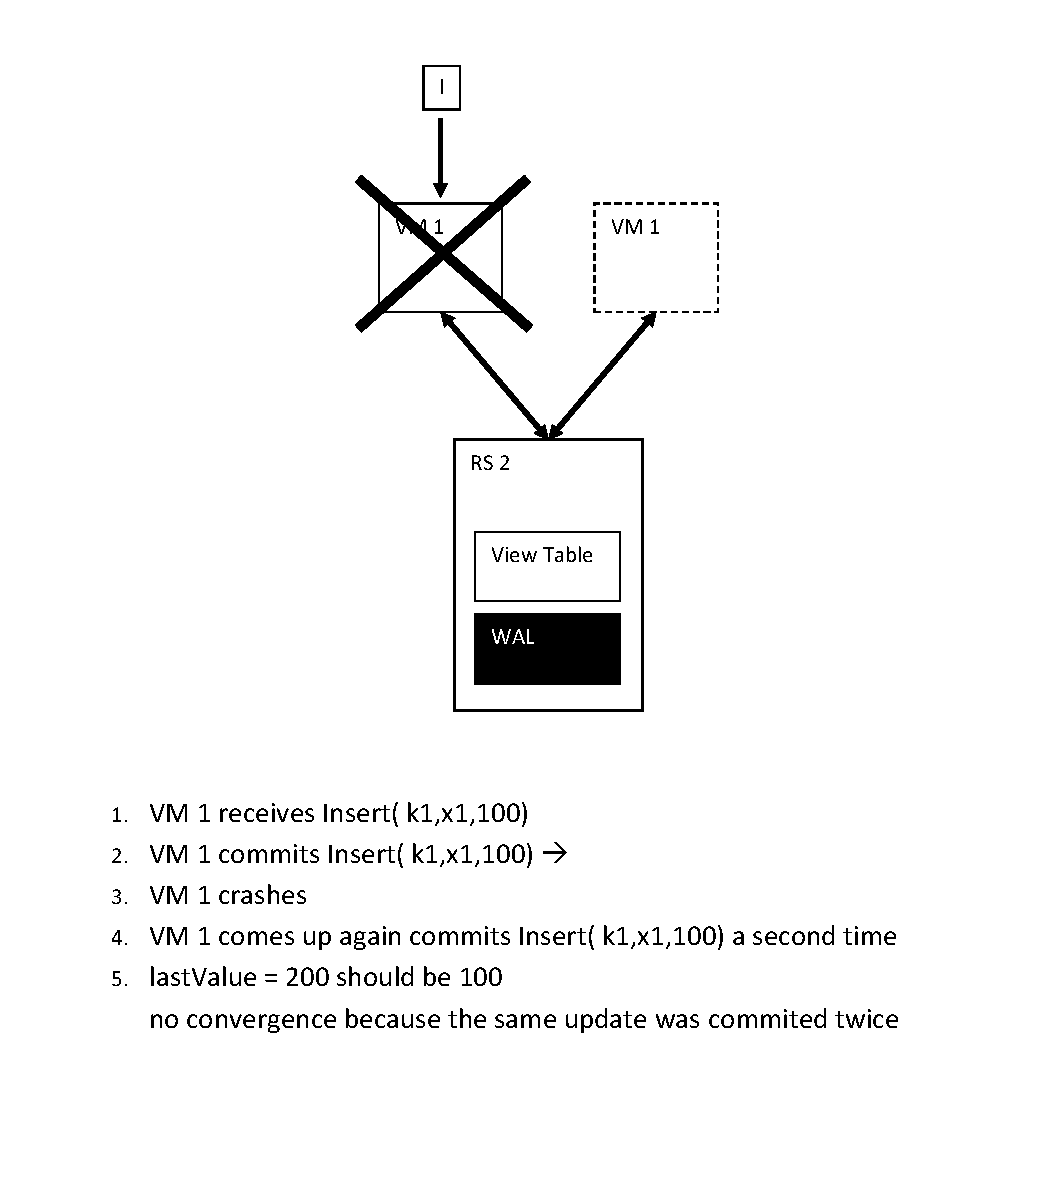
\includegraphics[scale=0.8]{figures/CO_NonIdempotentViewUpdates}
     \caption{Non idempotent view update}
    \label{fig:co_nonidempotentviewupdates}
\end{figure}

\newpage

\subsection{Wrong update order}
\begin{figure}[h!]
  \centering
    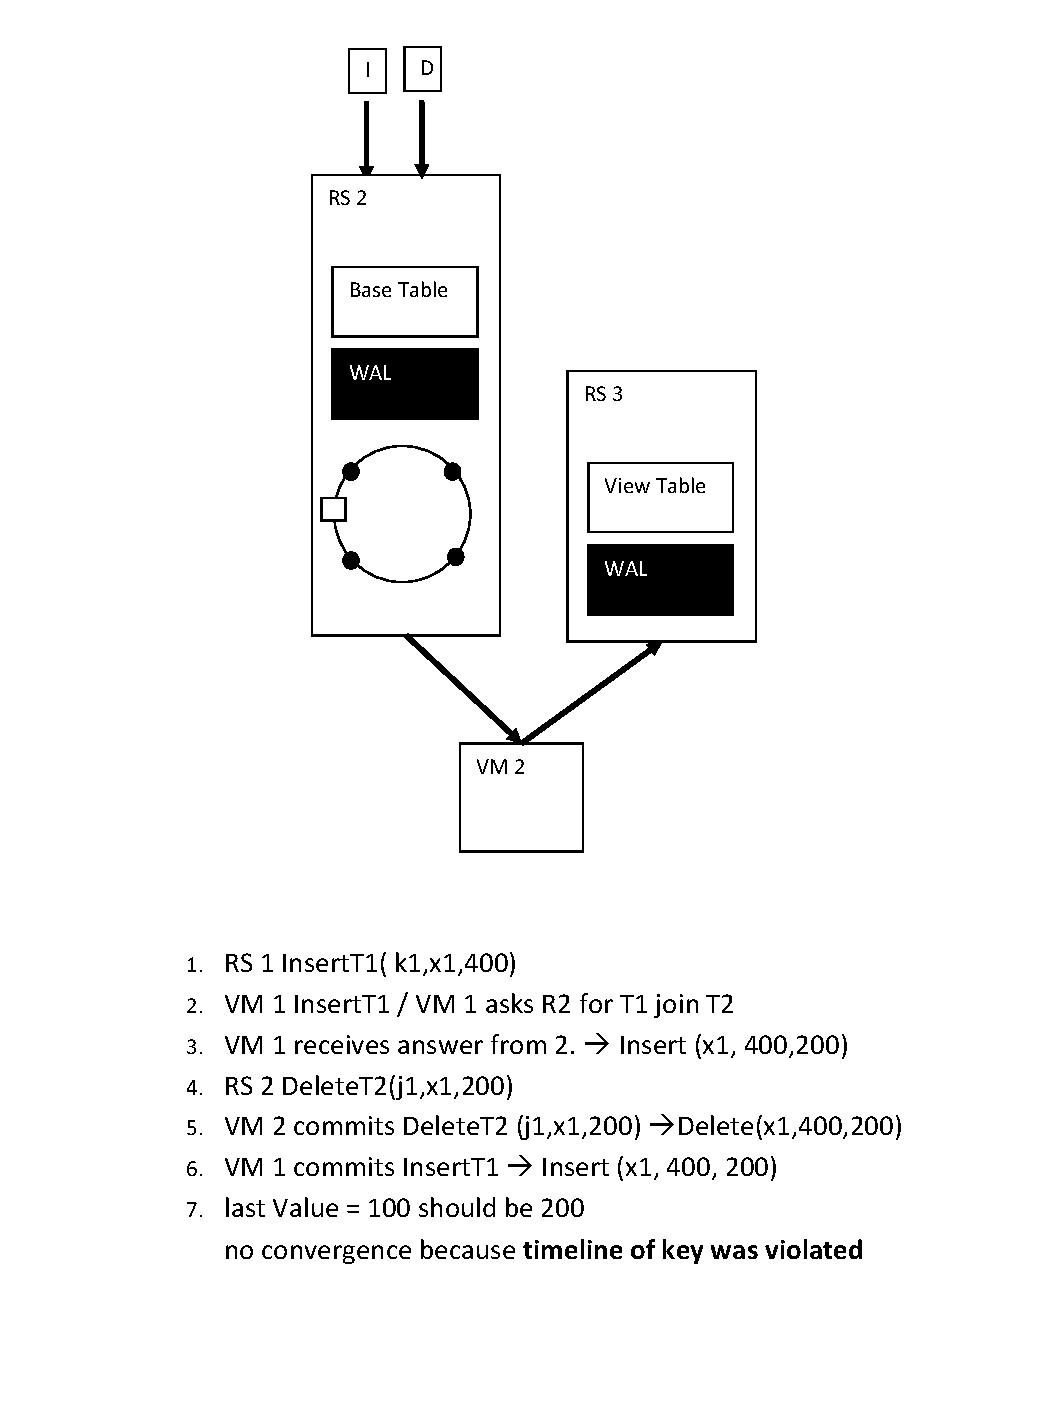
\includegraphics[scale=0.8]{figures/CO_WrongUpdateOrderJoin}
     \caption{Wrong update order join}
    \label{fig:co_wrongupdateorderjoin}
\end{figure}
\newpage
\begin{figure}[h!]
  \centering
    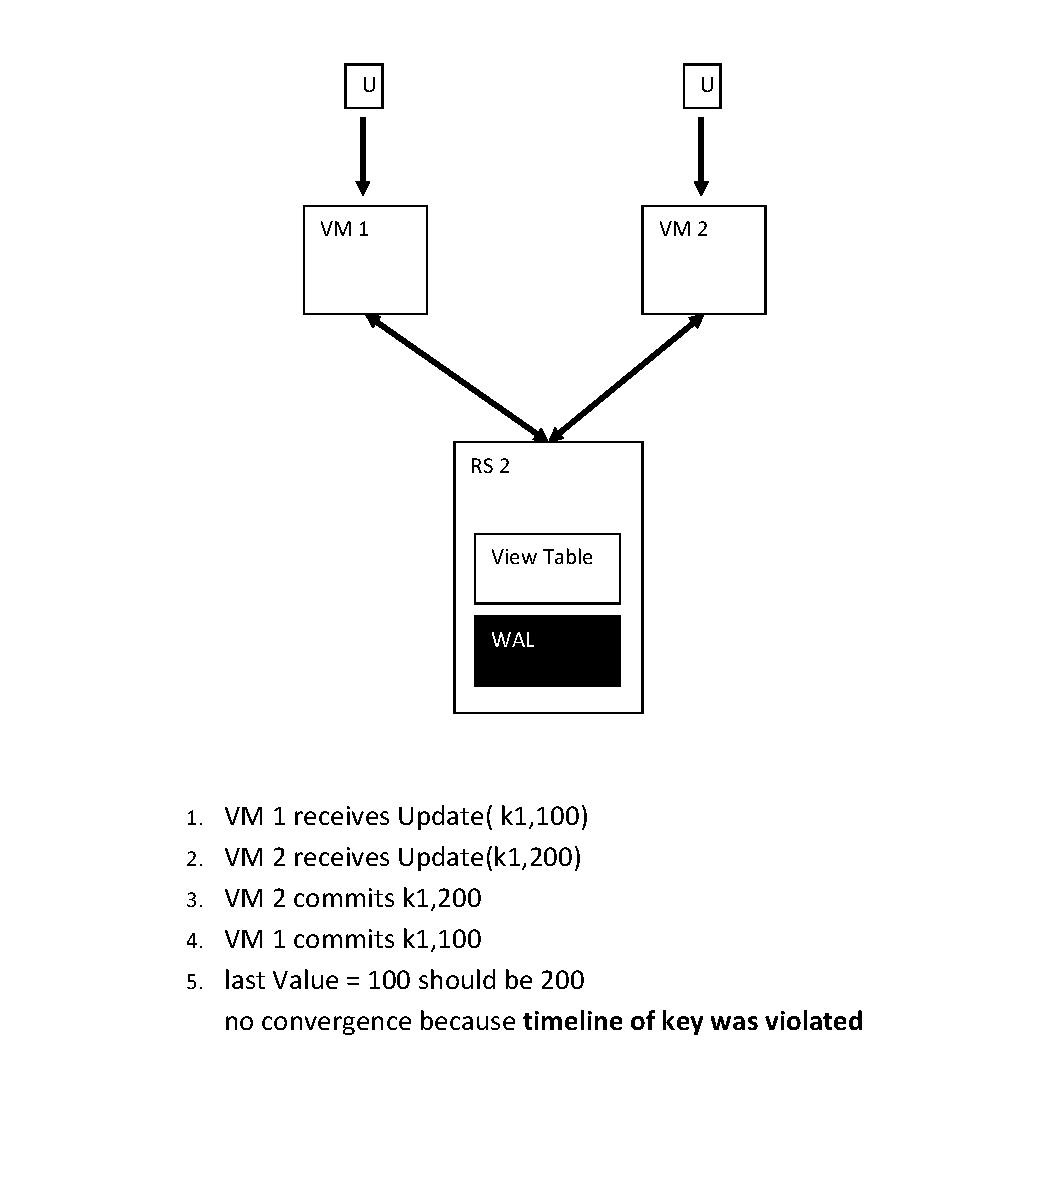
\includegraphics[scale=0.8]{figures/CO_WrongUpdateOrderSelection}
     \caption{Wrong update order Selection}
    \label{fig:co_wrongupdateorderselection}
\end{figure}
\newpage

\subsection{Concurrent commit}
\begin{figure}[h!]
  \centering
    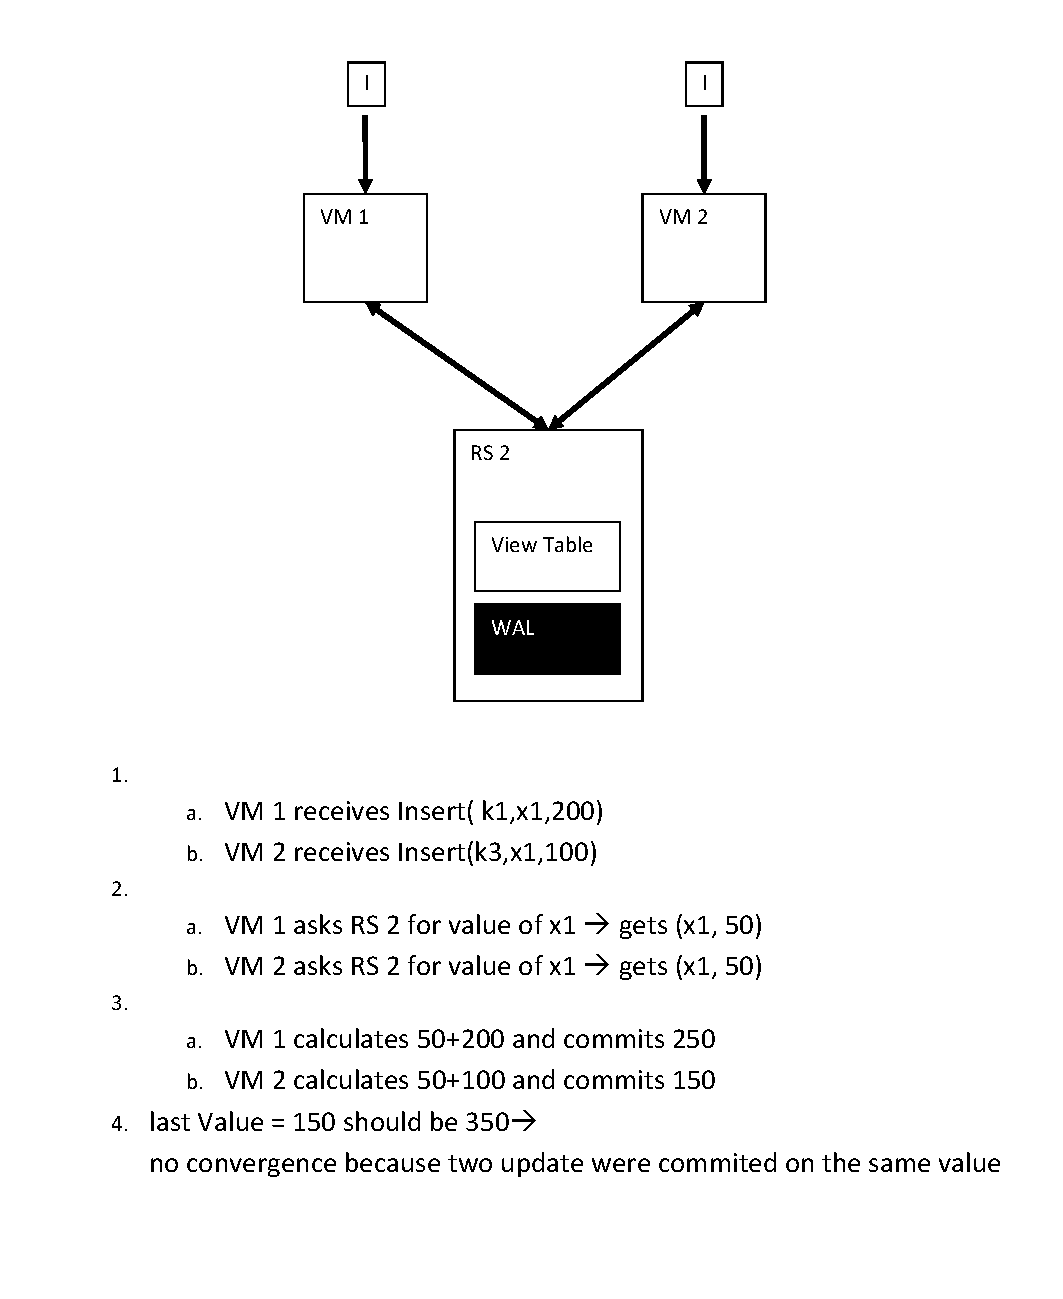
\includegraphics[scale=0.8]{figures/CO_ConcurrentCommitSum}
     \caption{Concurrent commit sum}
    \label{fig:co_concurrentcommitsum}
\end{figure}
\newpage
\begin{figure}[h!]
  \centering
    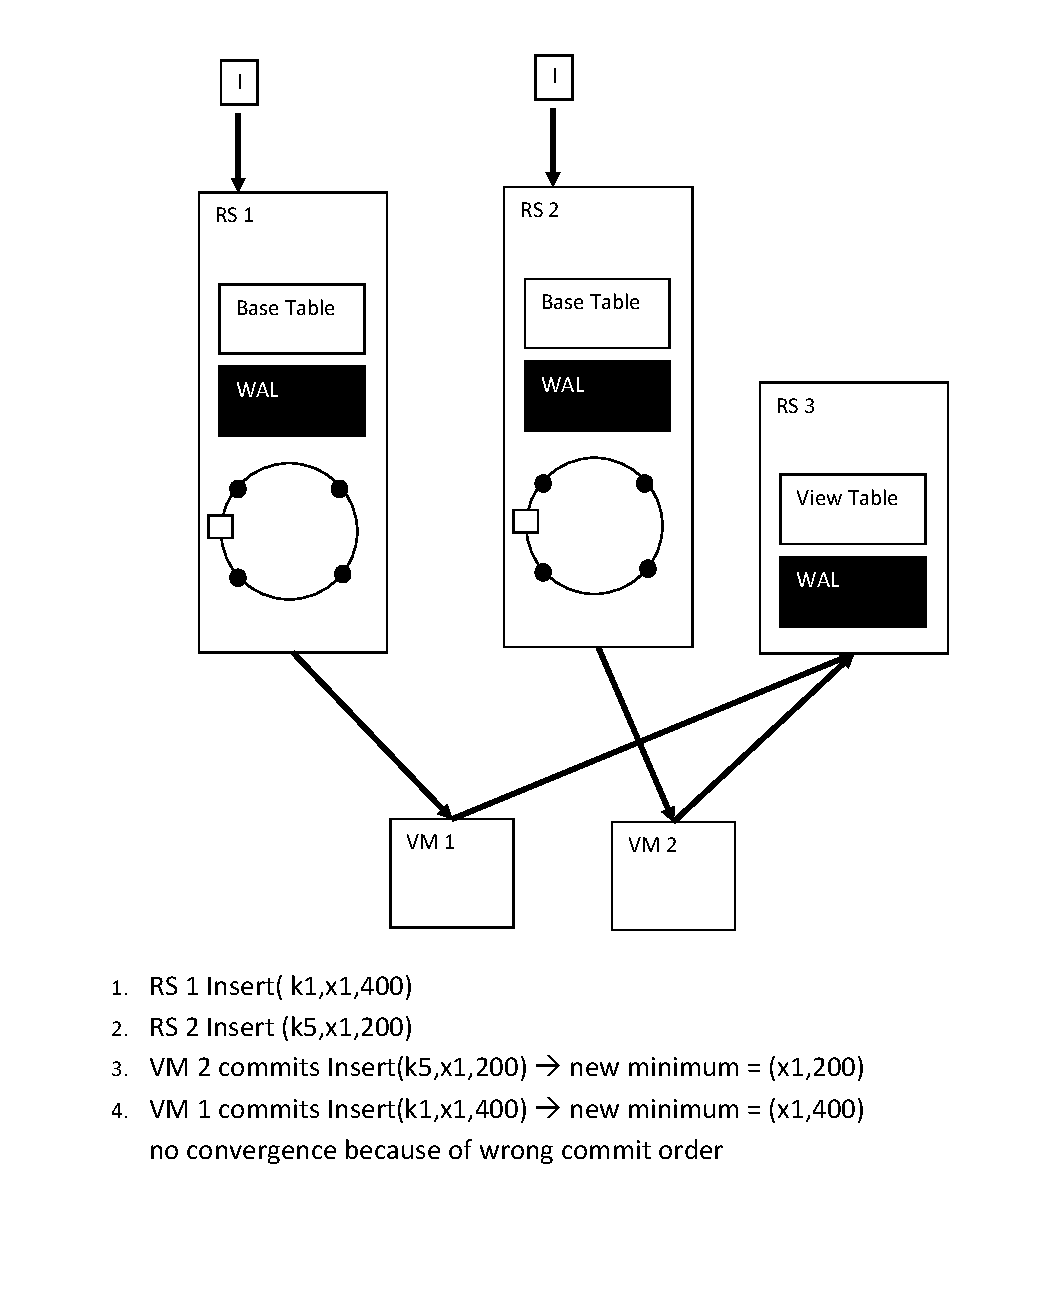
\includegraphics[scale=0.8]{figures/CO_ConcurrentCommitMin}
     \caption{Concurrent commit min}
    \label{fig:co_concurrentcommitmin}
\end{figure}
\newpage

\subsection{Update interference}
\begin{figure}[h!]
  \centering
    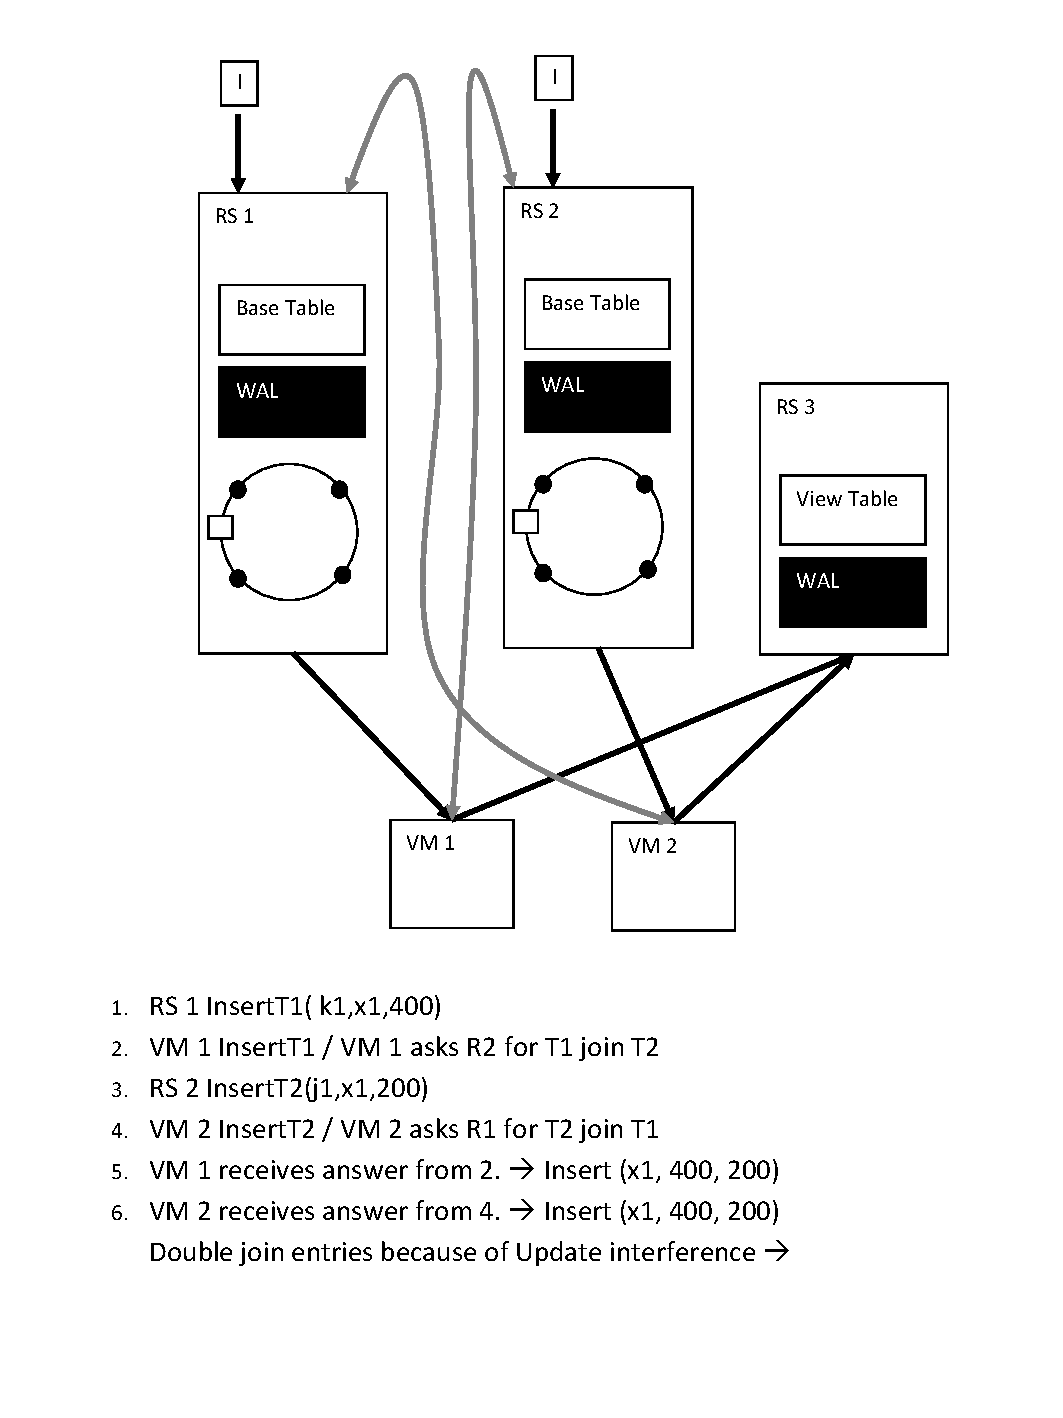
\includegraphics[scale=0.8]{figures/CO_UpdateInterferenceJoin}
     \caption{Update interference join}
    \label{fig:co_updateinterferencejoin}
\end{figure}
\newpage
\begin{figure}[h!]
  \centering
    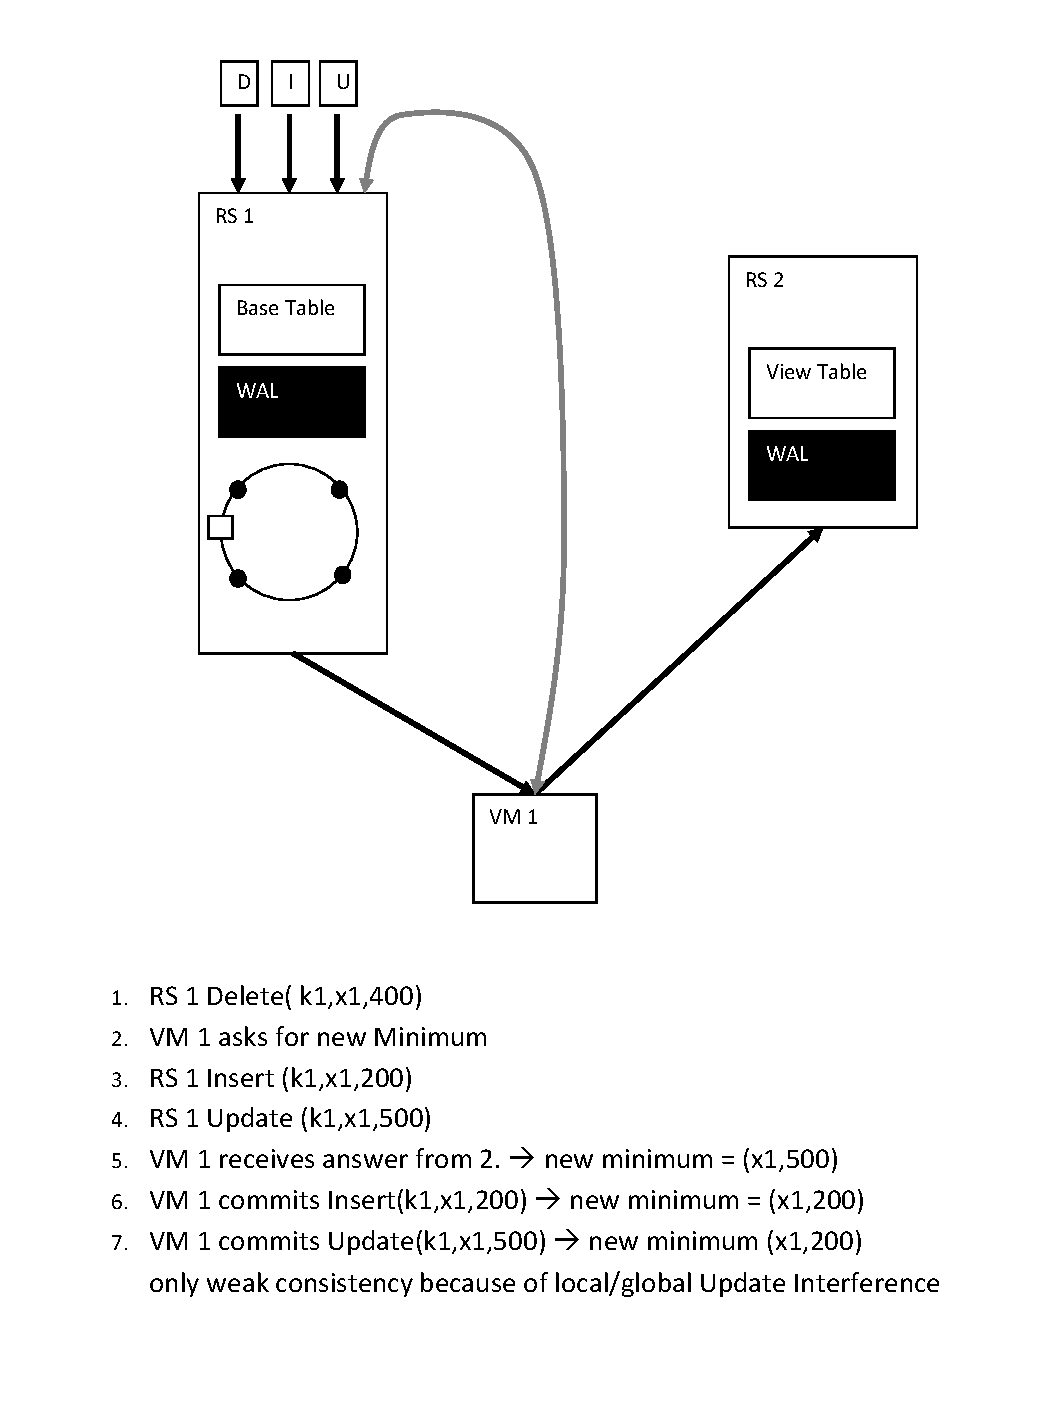
\includegraphics[scale=0.8]{figures/CO_UpdateInterferenceMin}
     \caption{Update interference min}
    \label{fig:co_updateinterferencemin}
\end{figure}
\newpage

\chapter{Load Balancing}
\label{chapter:loadbalancingappendix}


\section{Add View Manager}
\begin{figure}[h!]
  \centering
    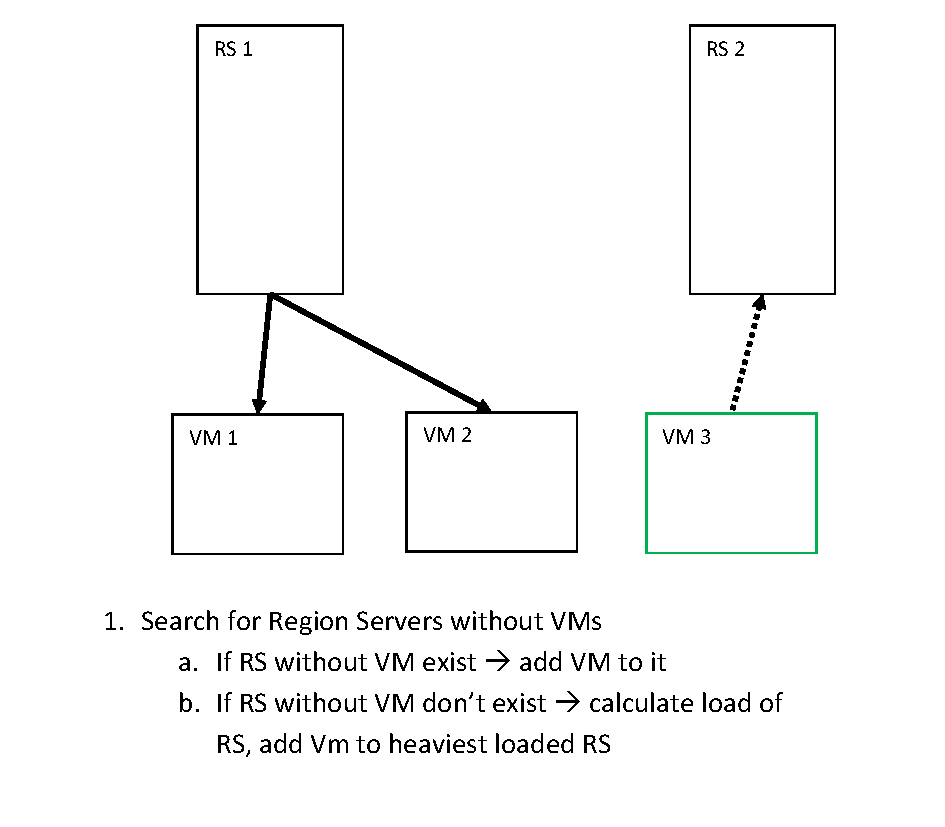
\includegraphics[scale=0.8]{figures/LB_AddViewManager}
     \caption{Add View Manager}
    \label{fig:lb_addviewmanager}
\end{figure}
\newpage

\section{Remove View Manager}
\begin{figure}[h!]
  \centering
    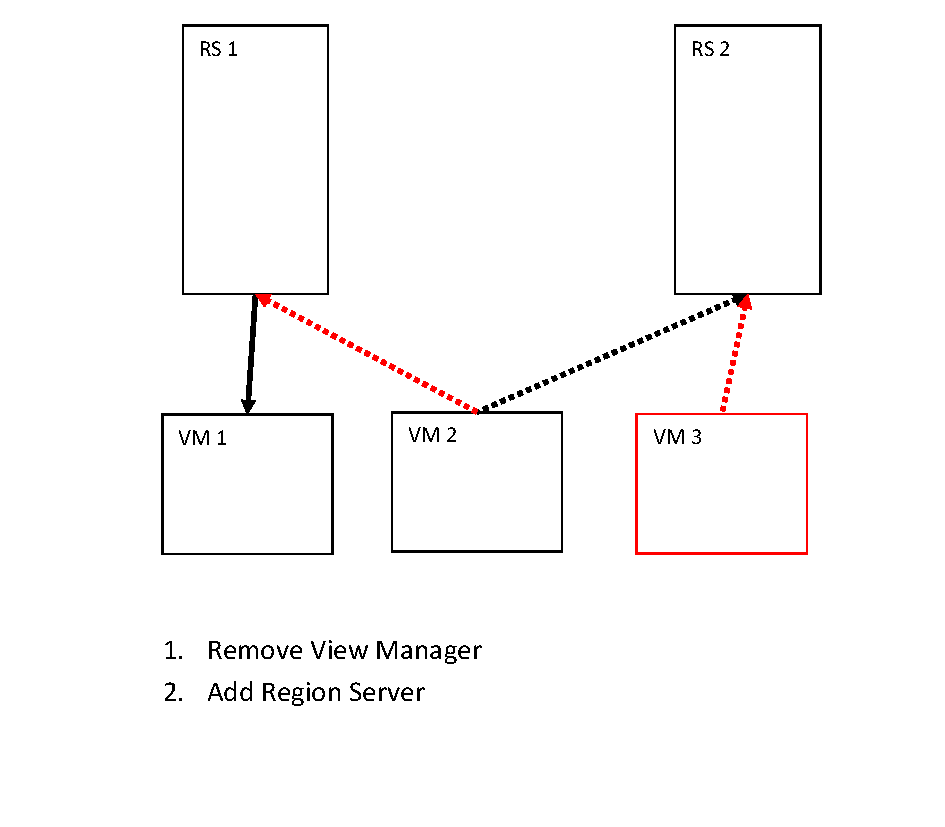
\includegraphics[scale=0.8]{figures/LB_RemoveViewManager}
     \caption{Remove View Manager}
    \label{fig:lb_removeviewmanager}
\end{figure}
\newpage

\section{Add Region Server}
\begin{figure}[h!]
  \centering
    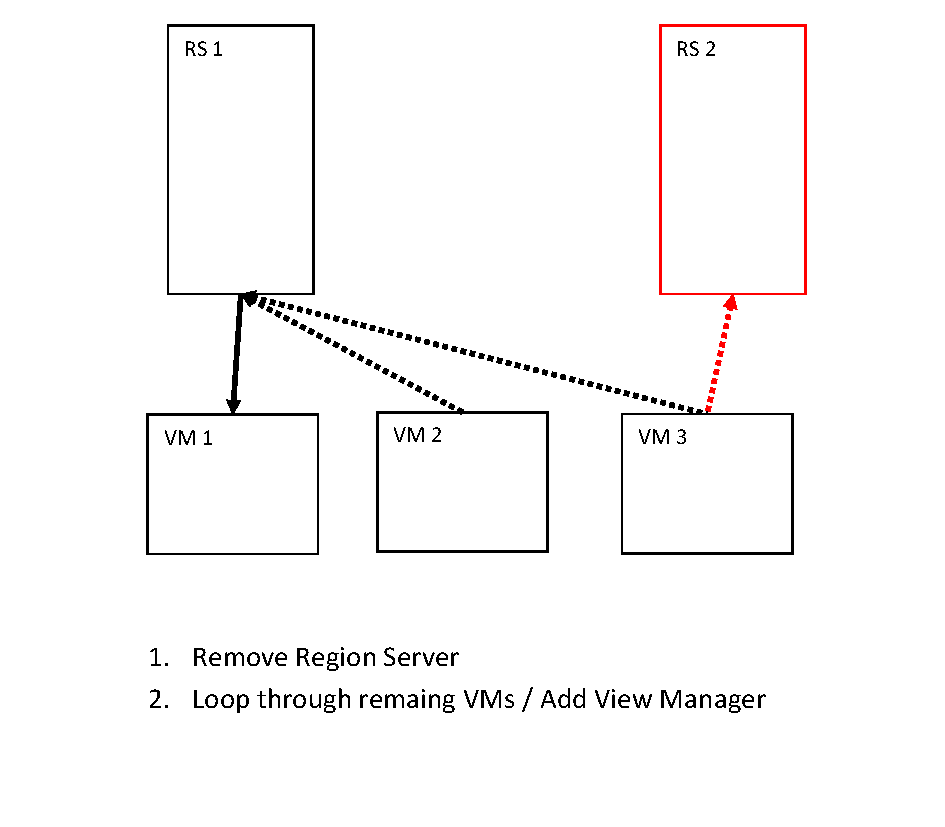
\includegraphics[scale=0.8]{figures/LB_AddRegionServer}
     \caption{Add Region Server}
    \label{fig:lb_addregionserver}
\end{figure}
\newpage

\section{Remove Region Server}
\begin{figure}[h!]
  \centering
    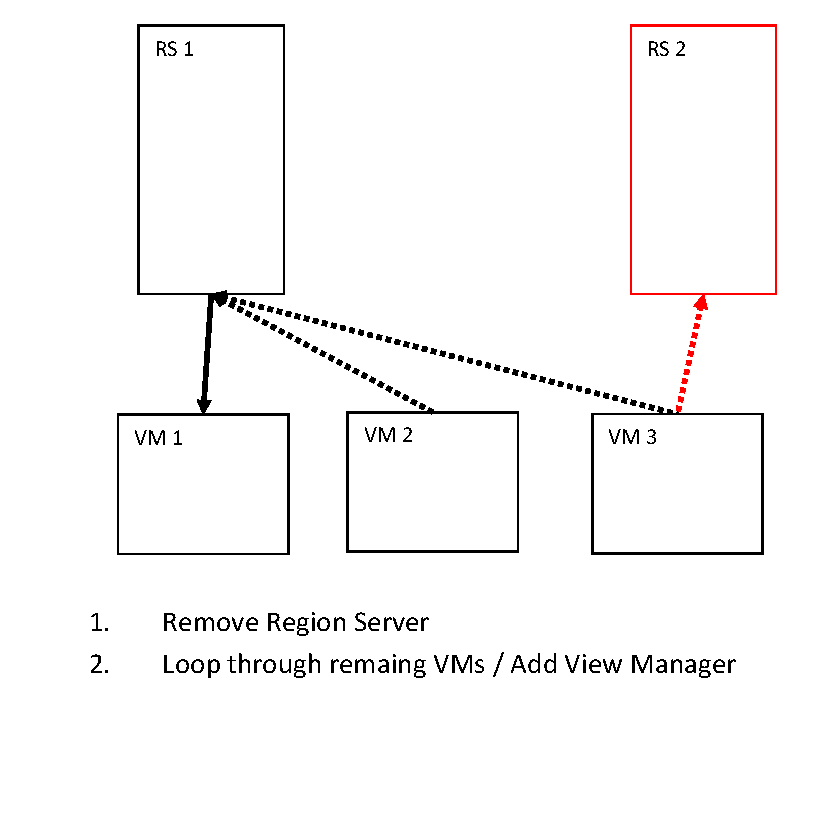
\includegraphics[scale=0.8]{figures/LB_RemoveRegionServer}
    \caption{Remove Region Server}
    \label{fig:lb_removeregionserver}
\end{figure}
\newpage




  \clearemptydoublepage
  
	\bibliography{bibliography/literature}
	
 
\end{document}

